%========================================================================
\newcommand*\dsk{./}

\newcommand*\figpath{\dsk/A_figs}
\newcommand*\bibpath{\dsk/A_bib}
\newcommand*\stypath{\dsk/A_style}
\newcommand*\chaptpath{\dsk/Chapt_v3}
\newcommand*\incpath{.}
%========================================================================

%========================================================================
%\documentclass[twoside,fontsize=11pt,headsepline,french]{scrbook}
\documentclass[twoside,fontsize=12pt,headsepline,english]{scrbook}
%========================================================================

%========================================================================

\usepackage{graphicx}   %% envir graphique pour latex ou pdflatex
%\usepackage[T1]{fontenc}     %% pour la cesure avec les accents
\usepackage[latin1]{inputenc} %% problemes d'accents
\usepackage[colorlinks=true, linkcolor=myred, citecolor=myred]{hyperref}         %% links dans le dvi
\usepackage{listings}

\usepackage{amsmath,amsfonts,amssymb}
\usepackage{mathrsfs}
\usepackage{amsthm}
\usepackage{pdfpages}	% % introduire plusieurs pages pdf
\usepackage{booktabs}	% % Tableau style

%\usepackage[sectionbib,gather]{chapterbib}       %%  pour la biblio locale (projet)
\usepackage{times}            %% pour pdf avec de jolie police
\usepackage{colordvi}        %% couleurs dans le dvi
%\usepackage[monochrome]{color}
\usepackage{color}
\usepackage{xcolor}
%\usepackage{amssymb,epic}
%\usepackage[french]{minitoc}   % mini-sommaires pour chaque chapitre
\usepackage{multimedia}       %% pour les films
\usepackage{array,multirow,makecell}  % pour fusionner les cellules dans un tableau
\usepackage{tabularx}

\usepackage{enumitem}
%========================================================================
%\usepackage[english]{babel}
%\usepackage[french]{babel}    %% style french
%------------------------------%% titres en francais
%\addto\captionsfrench{\renewcommand{\figurename}{\em Figure}%
%\renewcommand{\tablename}{\em Tableau}%
%\renewcommand{\chaptername}{\em }
%\renewcommand{\summaryname}{Sommaire}}
%========================================================================
%\usepackage{\stypath//floatflt}         %% figures dans les paragraphes -- il est nul
%=======================================biblio en anglais(non compat avec cite)
\usepackage[round]{natbib}
%\usepackage[]{natbib} 

%\bibliographystyle{plainnat}
%                     \cite{}     %citation normale
%                     \citet{}    %textuel
%                     \cite[texte avant][texte apres]{}
%                     \citep{}    %avec parenth{\`e}ses
%                     \citealt{}, \citealp{}    %sans aucune parenth{\`e}se
%                      \citeyear{},\citeauthor{}
%
%=======================================biblio en francais
%\bibliographystyle{\stypath//plainnat-io}
%\bibliographystyle{abbrvnat-fr} % biblio style francais
%\usepackage{\stypath//frbib}
%\bibliographystyle{\stypath//frcomplet}
%%%%%%%%%%========================================================================
%   --- couleurs
\definecolor{myred}{rgb}{0.8,0.1,0.1}

\def\textRed{\color{red}}
\def\textBlack{\color{black}}
\def\textBlue{\color{black}}
\def\Blue#1{{\color{black}{#1}}}
\def\Red#1{{\color{red}{#1}}}
\def\Darkred#1{{\color{red}{#1}}}
\def\Green#1{{\color{green}{#1}}}
\def\Magenta#1{{\color{magenta}{#1}}}
%========================================================================
%========================================================================
% 
\def\vv{{\vec v}}
\def\vva#1{\vec{#1}}
\def\ds{\displaystyle}
\def\pl{\partial}

\renewcommand{\vec}[1]{\boldsymbol{#1}}

\newcommand{\Rey}{{\cal R}e}
\newcommand{\Prd}{{\cal P}r}
\newcommand{\Ray}{{\cal R}a}
\newcommand{\Nuss}{{\cal N}u}
%\newcommand{\Gra}{{\cal G}r}
\newcommand{\Bou}{{\cal B}o}
\newcommand{\Ste}{{\cal S} te}
\newcommand{\vref}{{\small ref}}

\newcommand {\R} {{\mathbb R}}
\newcommand {\N} {{\mathbb N}}
\newcommand {\C} {{\mathbb C}}
\newcommand {\Z} {{\mathbb Z}}
\newcommand{\ie}{{\em i.\thinspace{}e. }}
\newcommand{\etal}{{\em et al. }}
\newcommand{\eg}{{\em e.\thinspace{}g. }}
\newcommand{\CKC}{C_{{\hbox{\tiny CK}}}}
\newcommand\widebar[1]{\mathop{\overline{#1}}}
\newcommand{\ff}{FreeFem{\small +$\!$+}  }
\newcommand {\PP} {{\mathbb P}}

\def\cels#1{#1\, ${^\circ}$C}
\def\celsm#1{#1\, {^\circ}\mbox{C}}

\newcommand{\bigO}[1]{\ensuremath{\mathop{}\mathopen{}O\mathopen{}\left(#1\right)}}
%========================================================================
%mise en page

\usepackage[hmargin={3cm,2.3cm},vmargin={3cm,3cm}]{geometry}

%\topmargin -1.54cm   %marge en haut a 2cm %% on monte de 1.65 cm car dvi2ps marche en letter 11in
%\oddsidemargin 0cm   %marge a 2 cm
%\evensidemargin 0cm  %marge a 2 cm
%\parindent 0.cm
%\parskip 0.3cm
%\headsep 0.5cm \topskip .5cm \footskip 1.5cm \headheight 1.0cm
%\textwidth  15cm \textheight 22cm

%-------- dimensions pour les cadres des exercices, theoremes, etc
\def\leftsymb{0.5cm}
\def\rightenv{\textwidth}

%\def\minileft{5.3cm}
%\def\miniright{10.5cm}
\def\onefig{\textwidth}
\def\onefigS{0.6\textwidth}
\def\onefigM{0.75\textwidth}
\def\onefigB{0.99\textwidth}
\def\twofig{0.5\textwidth}
\def\threefig{0.33\textwidth}

\newtheorem{thm} {Th�or�me} [section]
\newtheorem{defi}[thm] {D�finition}
\newtheorem{prop} [thm] {Proposition}
\newtheorem{rem}[thm] {Remarque}
\newtheorem{concl}[thm] {Conclusion}
%%%%%%%%%%%%%%%%%%%%%%%%%%%%%%%%%%%%%%%%%%%%%%%%%%%%%%%%%%%%%%%%%%%%%%%%%%%%%%%
%%%%%%%%%%%%%%%%%%%%%%%%%%%%%%%%%%%%%%%%%%%%%%%%%%%%%%%%%%%%%%%%%%%%%%%%%%%%%%%
\def\LOGO{\hbox{\includegraphics[scale=0.75]{\stypath/logo-lmrs125.jpg}}}
\font\fonteupmc=pagk at 10 true pt
\font\plutotgros=pagk at 12 true pt
\def\LAN{\plutotgros}
\def\upmc{\fonteupmc}

\def\entete{
\vbox {
\hbox to \hsize{%
\hskip -1 cm\vbox{\LOGO}\hskip 0.45 true cm \vbox{\hbox{\LAN
Laboratoire de math�matiques Raphael Salem} \vskip .2 true cm \hbox{\upmc
Universit� de Rouen} \vskip .5 true cm
\hbox{\upmc Avenue de l'Universit�, BP.12,
  76801 Saint-�tienne-du-Rouvray}}
 \hfill}
 {\vskip .9 true cm
\hbox{\hskip -1 cm} \vskip .1 true cm
\hbox{\hskip -1 cm}}}}

%%%%%%%%%%%%%%%%%%%%%%%%%%%%%%%%%%%%%%%%%%%%%%%%%%%%%%%%%%% 
%%%%%%%%%%%%%%%%%%%%%%%%%%%%%%%%%%%%%%%%%%%%%%%%%%%%%%%%%%%%%%%%%%%%%%%%%%%%%%%
%%%%%%%%%%%%%%%%%%%%%%%%%%%%%%%%%%%%%%%%%%%%%%%%%%%%%%%%%%%%%%%%%%%%%%%%%%%%%%%
%\titlehead{\hspace{1.5cm}\entete}
%\title{\vspace{-1cm}
%	\huge\Magenta{
%	Numerical simulation of phase-change materials.
%}\\

%{\includegraphics[width=0.35\textwidth]{\figpath/figs_bose/lattice_3.jpg}}
%}

\usepackage{orsay-title}

%\author{\Large \Blue{Aina Rakotondrandisa} }
\author{Aina \textsc{Rakotondrandisa}}

%\subject{\vspace{-2cm} Preliminary report}
%\date{}

\title[french]{Mod�lisation et simulation num�rique des mat�riaux � changement de phase}
%Titles for other languages
\title[english]{Modeling and numerical simulation of solid-liquid phase-change material}

%Keywords for main language (french)
\keywords[french]{}
%Keywords for other languages languages
\keywords[english]{}

\ordernumber{1234}

%\publishers{\small
%\begin{flushleft}
%	\Blue{This document is intended to evolve by gradually adding contributions. Feel free to correct or add parts to the latex source file, eventually using colors.} \Red{red}, \Blue{blue}, \Green{green}, etc.\\
%	The purpose of this study is twofold:
%	\begin{enumerate}
%	\item Evaluate the accuracy in time and space of the finite-element solver for phase change systems.\\ Idea: manufactured solutions will be used to estimate the space accuracy (stationary Burggraf flow) and time-dependent manufactured solution (as in \cite{nourgaliev2016fully}) for the time accuracy.
%	
%	\item Try to find an equivalence between the two models used to take into account the solid phase inside a single-domain approach: the viscosity penalty used in \cite{dan-2014-JCP} and the well-know Carman-Kozeny model (\eg \citep{belhamadia2012}).\\ Idea: study the mathematical derivation of the  Carman-Kozeny model from the Darcy equations; study the behaviour of the CK model compared to the viscosity penalisation for simple models/configurations (melting of a PCM).
%
%\end{enumerate} 	 
%\end{flushleft}
%}

\begin{document}
%%%%%%%%%%%%%%%%%%%%%%%%%%%%%%%%%%%%%%%%%%%%%%%%%%%%%%%%%%%%%%%%%%%%%%%%%%%%%%%%

%
%\renewcommand{\refname}{Bibliography of chapter }
%\renewcommand*\partformat    {\partname~\thepart: } % regle le pb titre partie
\renewcommand*\partformat    {\thepart } % regle le pb titre partie
%%%%%%%%%%%%%%%%%%%%%%%%%%%%%%%%%%%%%%%%%%%%%%%%%%%%%%%%%%%%%%%%%%%%%%%%%%%%%%%%
%%%%%%%%%%%%%%%%%%%%%%%%%%%%%%%%%%%%%%%%%%%%%%%% initialisation minitoc
%\doparttoc %Table of contents for parts
%\dopartlof List of figures for parts
%\dopartlot List of tables for parts
%\dominitoc %Table of contents for chapters
%\dominilof List of figures for chapters
%\dominilot List of tables for chapters
%\dosecttoc Table of contents for sections
%\dosectlof List of figures for sections
%\dosectlot List of tables for sections


%%%%%%%%%%%%%%%%%%%%%%%%%%%%%%%%%%%%%%%%%%%%%%%%%%%%%%%%%%%%%%%%%%%%%%%%%%%%%%%%
%\maketitle


%%%%%%%%%%%%%%%%%%%%%%%%%%%%%%%%%%%%%%%%%%%%%%%%%%%%%%%%minitoc commands
%\parttoc Table of contents for parts
%\partlof List of figures for parts
%\partlot List of tables for parts
%\minitoc Table of contents for chapters
%\minilof List of figures for chapters
%\minilot List of tables for chapters
%\secttoc Table of contents for sections
%\sectlof List of figures for sections
%\sectlot List of tables for sections
%%%%%%%%%%%%%%%%%%%%%%%%%%%%%%%%%%%%%%%%%%%%
%%%%%%%%%%%%%%%%%%don't forget if needed %%%%%%%%%%%%%%%%%%%%%%%%%%%%%%%%%%%%%
%\chapter[toc version]{title version}
%\chaptermark{head version}
%\section[toc version]{title version%
%              \sectionmark{head version}}
%\sectionmark{head version}
%%%%%%%%%%%%%%%%%%don't forget if needed %%%%%%%%%%%%%%%%%%%%%%%%%%%%%%%%%%%%%

\frontmatter


%Print title NOW
\maketitle%

%Disable page numbering
\pagestyle{empty}

%########################################################################
% Multilingual abstracts

\begin{abstract}[english]
%\dummytext
To be completed at the end
\end{abstract}

%%Horizontal rule
\noindent\hspace*{0.35\textwidth}\hrulefill\hspace*{0.35\textwidth}\\[-\bigskipamount]


%French abstract:
\begin{abstract}[french]
%\dummytext
Nous proposons dans cette �tude une nouvelle approche ...
\end{abstract}

%########################################################################



%########################################################################
% Contents
%########################################################################

%\strut\newpage
\small
\tableofcontents

\newpage

%%%%%%%%=====================================================
%\pagestyle{myheadings}
\pagestyle{headings}
\renewcommand*{\chaptermarkformat}{%
\chapapp~\thechapter\autodot\enskip}


%%%%%%%%=====================================================
\mainmatter
%%%%%%%%%%%%%%%%%%%%%%%%%%%%%%%%%%%%%%%%%

%%%%%%%%%%%%%%%%%%%%%%%%%%%%%%%%%%%%%%%%%%%%%%%
%%%%%%%%%%%%%%%%%%don't forget if needed %%%%%%%%%%%%%%%%%%%%%
%\section[toc version]{title version%
%              \sectionmark{head version}}
%\sectionmark{head version}
%%%%%%%%%%%%%%%%%%%%%%%%%%%%%%%%%%%%%%%%%%%%%%%%%%%%%%%%%%%%%%
\def\titcourt{Introduction}
\def\titlong{Introduction}
%%%%%%%%%%%%%%%%%%%%%%%%%%%%%%%%%%%%%%%%%%%%%%%%%%%%%%%%%%%%%%%%
\chapter[\titlong]{\titlong%
              \chaptermark{\titcourt}}
\chaptermark{\titcourt}
%%%%%%%%%%%%%%%%%%%%%%%%%%%%%%%%%%%%%%%%%%%%%%%%%%%%%%%%%%%%%%%%
%%%%%%%%%%%%%%%%%%%%%%%%%%%%%%%%%%%%%%%%%%%%%%%%%%%%%%%%%%%%%%%%

Climate change is more than ever experienced in our daily life:
irregular melt of sea, deterioration of ozone layer, non-seasonal precipitation, etc.
Our dependency on fossil fuels during the last decades for energy production have caused severer environmental issues.
%Notwithstanding these alarming phenomenon, those energy sources is still causing severer environmental issues.
%The world's energy consumption was fully dominated by , and 
As it is illustrate in Fig. \ref{fig-Energ-cons}a,  coal and natural gas are the main energy sources for electricity generation in the world in 2017 \citep{dudley2018bp}. 
Today, we must face to the fact that these fossil fuels are going to an end and admit that their large utilization has induced considerable impacts on our environment.
%Notwithstanding until today, our dependency on those energy sources is still causing severer environmental issues.
%Climate changing, mostly due to the huge CO2 and other green house gases released into the atmosphere, is more than ever experienced in our daily life:
%unnatural heat waves, non-seasonnal precipitation, seal level rising, increasing melt of sea ice, deterioration of ozone layer, etc.

\begin{figure}[!h]
\begin{center}
	\begin{minipage}{.49\textwidth}
		(a) \\
		\includegraphics[width=\textwidth]{\figpath/Fig_cap_introduction/Energy_by_continent_2}
	\end{minipage}
		\begin{minipage}{.50\textwidth}
		(b) \\
		\includegraphics[width=\textwidth]{\figpath/Fig_cap_introduction/Energy-residential-EU}
	\end{minipage}
	\caption{(a) Electricity generation by different energy sources in 2017 by different continent by \cite{dudley2018bp}. (b) Energy use repartition in a residential buildings in Europe by \cite{dudley2018bp}.}
	 \label{fig-Energ-cons}
\end{center}	
\end{figure}

\noindent Research on environment-friendly energy sources, such as biomass, wind or solar have attracted many considerations recently.
Even though solar or wind energy are now operational, their main drawback remains the gap between their availability and the consumers demand.
Solar energy is not available during the nights for example, while wind energy is intermittent over the year.
The energy demand varies with time and the energy suppliers have to meet this demand.
An efficient solution to this discrepancies of availability and demands problem is the use of energy storage systems.
The idea is to store the energy at one time in one form or another and release it latter for a particular need, since energy availability and demand rarely concur.
The energy storage process is a crucial point for renewable and sustainable energy.
The later can be divided into five classes:
magnetic, biological, chemical, mechanical and thermal energy storages.
The main feature of the aforementioned energy storage technologies relies on energy charging and discharging process.
In most cases however, thermal energy is the energy form widely used.
Even the electricity generation is monitored by heat generating high temperature and high pressure.
Storing thermal energy is hence an efficient and fundamental way to store the energy.
It can be realised by rising the substance's temperature (sensible heat energy storage) or by changing the substance's phases (latent heat energy storage).


\begin{table}[!h]
	\begin{center}
		\begin{tabular}{ccccc}
			Agriculture & Buildings & Industry  & Transportation & Other  \\ \hline
			4.5 & 41.8 & 26 & 43.8 & 4.5 \\
		\end{tabular}
	\end{center}
	\caption {The energy consumed by different domain in France in 2017, in million tonne of oil equivalent. French ministry of ecological transition \citep{ministereEcologie2018}.}
	\label{tab-french-min}
\end{table}

Research on passive heat storage system have attracted many considerations lastly, namely interest on Phase Change Material (PCM) as latent heat energy storage have arisen.
PCM are used to store heat during the melting of the materials and releases later the stored heat during the solidification process.
At present, the latent heat storage technologies are proven as an effective solution to decrease the use of fossil fuel and in the same time increase the energy usage efficiency.


Aside from energy storage technologies, PCMs are also widely used in building applications, to decrease the temperature fluctuations.
Latest announcement of the french ministry of ecological transition, detailing the repartition of the energy consumption in different domains, indicates more than $35 \%$ of the total energy being consumed by residentials and commercial buildings. Details about energy consumptions in 2017 are shown in Tab. \ref{tab-french-min}.
More than $60\%$ of the total energy consumption in residential sector is dedicated to space heating (see Fig. \ref{fig-Energ-cons}b).
Research towards energy-efficient building to reduce heating and cooling demand is of principal interest nowadays.
Taking advantage of the high value of the latent heat of solid-liquid transformations, PCMs are widely encountered in thermal regulation in buildings to reduce overheating.
In summer, PCMs are used to absorb the excessive solar radiation heat and maintain a bracing indoor ambience.
PCM with a temperature of fusion close to the ambient temperature is generally used to ensure a melting during the daytime and a solidification during the nighttime.
During winter however, PCMs can be used to store heat generated by electrical heating system during the night and then release it in the daytime.

%The use of efficient insulation is the key of energy conservation in residential buildings.

\begin{table}[!h]
	\begin{flushleft}
		\begin{tabularx}{\linewidth}{cXX}
					Temperature range & PCM & Target application area \\ \hline \hline
			0 - 65 $^o C$ &    Paraffins (-3 to 64 $^o C$), water / ice  (0 $^o C$), stearic acide  (41 - 43 $^o C$), {n-octadecane  (27.7 $^o C$)}   &   Storage for domestic heating/cooling. Passive storage in bio-climatic building/architecture. Thermal storage of solar energy. Application in off-peak electricity for cooling and heating. Protection of electrical devices.\\ \hline
			%80 - 120 $^o C$ & Erythritol (117.7 $^o C$), RT100  (99 $^o C$),  $MgCl_2 6H_2 O$& \\ \hline
			80 - 120 $^o C$ &    Erythritol (117.7 $^o C$), RT100  (99 $^o C$), $MgCl_2 \, 6H_2O$  (116.7 $^o C$)   &   Storage for the hot-side of $LiBr/H_2O$ absorption cooling system with generator temperature requirements of less than 120 $^o$C\\ \hline
			$ > 150 $ $^o C$ &    $NaNO_3$ (310 $^o C$), $KNO_3$  (330 $^o C$), $NaOH$  (318 $^o C$),  $KOH$  (380 $^o C$), $ZnCl_2$  (280 $^o C$)  &   Storage for solar power plants based on parabolic trough collectors and direct steam generation.\\ 

		\end{tabularx}
	\end{flushleft}
	\caption {Target application area for some PCM studied in the literature \citep{agyenim2010review}.}
	\label{tab-PCM-app}
\end{table}

Phase-change problems are a very timely subject and is encountered in a wide range of applications ranging from metal casting and passive temperature control devices (e. g. for modern portable electronics), to food freezing and cryosurgery.
In many PCMs applications, the choice of an appropriate material for a specific application depends of many criteria, such as the operating temperature range, the thermal conductivity, the costs, etc.
They are generally classified into three classes: organic, inorganic and eutectic.
A target application area for some PCM are drawn in Tab. \ref{tab-PCM-app}.
The main operating temperature range can be assorted by three groups. First, $0$ to $65 ^o C$ for thermal storage used in domestic heating/cooling or for thermal storage of solar energy. Paraffins and water are used for such applications.
Second, $80$ to $120 ^o C$ for the cooling of systems with generator temperature of less than $120 ^o C$ purpose.
Finally, greater than $150 ^o C$ for the heat storage in solar power plants based on parabolic trough collectors and direct steam generation.

Melting and solidification are also fundamental process in geophysical problem such as Earth's mantle formations, lava lakes \citep{davaille1993thermal}, thermal convection in magma chambers \citep{brandeis1989convective} or ice-melt lakes \citep{polashenski2012mechanisms}. Ice-melt ponds that form during summer season in the Arctic \citep{polashenski2012mechanisms,esfahani2018basal} are known for example to display natural convection coupled to a phase-change process on the bottom side. In that case, Rayleigh-B�nard like convection cells are observed in the liquid phase.

The solid-liquid phase-change phenomenon is a very complex process. 
It couples the natural convection in the liquid phase induced by the buoyancy force, the non-linear evolution of the phase-change interface and the heat transfer process, which could be different from one configuration to another.
The coupling of all these physical phenomenons induce strong non-linear process in the solid-liquid problems, difficult to analyse except for simple and ideal test cases.
Fig. \ref{fig:expe-PCM_Gong} showing the experimental investigation of the melting of n-octadecane inside a transparent brick by \cite{gong2015numerical} depicts very well the complexity of the problem.
The investigated material is heated from the right and melts from the right to the left.
Figs. \ref{fig:expe-PCM_Gong}a and \ref{fig:expe-PCM_Gong}b depict the evolution of the liquid fraction and the vector field in the fluid obtained by particle image velocimetry (PIV) method.
Capturing accurately the non-linear evolution of the solid-liquid interface, due to the strong convection in the melting PCM, is clearly a challenging numerical task.
Furthermore, the existence of boundary layers near the walls and the interface is also illustrated in Fig. \ref{fig:expe-PCM_Gong}b suggesting that the mesh resolution should allow to capture these structures.

\begin{figure}[!h]
	\begin{center}
		\includegraphics[width=\textwidth]{\figpath/Fig_cap_melting/EXPE_GONG_melting}
	\end{center}
	\caption{Experimental observation of the melting of n-octadecane within a transparent brick of plexiglas heated vertically from the left by \cite{gong2015numerical}, obtained by particle image velocimetry (PIV) method.}
	\label{fig:expe-PCM_Gong}
\end{figure}

Other the past $30$ years, solid-liquid phase-change has been widely studied. % using either numerical, analytical, or experimental methods.
Rectangular and cylindrical geometries were the most investigated configuration.
\cite{Okada1984,gau1983flow,gong2015numerical} have investigated experimentally the melting of octadecane and gallium PCMs inside rectangular containers.
\cite{ho1984inward,liu2014experimental,omojaro2017study} have studied experimentally the melting of different paraffin within cylindrical enclosures.
These experimental investigations have been extensively used for numerical validation (see \cite{bertrand1999melting,gobin2000melting,wang2010numerical,dan-2014-JCP,rakotondrandisa2019numerical}) and have permitted a better comprehension of the physical phenomenon that occurs during melting and solidification, mainly the heat transfer process.
%The experimental results are very often formulated in the form of mathematical correlations.
Experimental work of \cite{Okada1984} have permitted for example to express correlations of the variation of dimensionless thermal energy stored as latent heat, and the average Nusselt number on the vertical wall with the dimensionless time.
Later, \cite{ho1984inward} have analyzed the solid-liquid interface position function of the configuration, \cite{jany1988scaling} have formulated $N\!u$-$\Ray$ correlation through a scaling analysis.
\cite{bejan1989analysis} gathered the previous observations and described analytically the solid-liquid melting process in the frame of vertical heating.

Gallium and n-octadecane are the most investigated materials. Experimentals \citep{gau1983flow,Okada1984,campbell1994visualization,gong2015numerical}, numericals \citep{rady1996natural,bertrand1999melting,hannoun2003resolving,Wang2010,dan-2014-JCP,rakotondrandisa2019numerical}, and theoreticals \citep{Okada1984,jany1988scaling,bejan1989analysis,kowalewski2004phase} were widely investigated. 
Besides their physical properties are equal in both liquid and solid phases (differences less than $3 \%$), gallium and n-octadecane melt near room temperature, making them the preferred materials for experimentally investigating melting and solidification of low and high Prandtl-number PCMs respectively.
%These problems in a rectangular cavity have been also extensively used in the literature for the assessment of phase-change numerical methods

The previously mentioned work were mostly focused on studying separately melting or solidification problems
and only recently for alternate melting and solidification complete cycles \citep{wang2010numerical,rakotondrandisa2019numerical}. 
Prior to these studies on complete cycles, periodic melting and solidification problems were the most studied in the literature. 
\cite{ho1993periodic} and \cite{voller1996cyclic} studied numerically, periodic melting in square enclosures. 
Recently, \cite{hosseini2014experimental} carried out melting and solidification of a cylindrical PCM during charging and discharging process and \cite{chabot2017solid} studied analytically the effect of an alternate heating and cooling in a cylindrical PCM, with periodical boundary conditions.
We have also contributed recently on the comprehension of the governing mechanism during the melting and the solidification in the paper \cite{rakotondrandisa2019numerical}.
We analyzed in detail the difference between solidification occuring after a partial melting and a complete melting by providing temporal evolution of solid-liquid interface, liquid fraction, Nusselt number and accumulated heat input. 

While publication about melting and solidification of PCM heated from the side is very abundant, research on melting of PCM heated from below is quite rare.
\cite{diaz1984visualization,hale1980solid} have studied experimentally the solid-liquid interface morphology of PCM during basal heating.
\cite{gong1998flow} studied numerically the flow and heat transfer during the melting of pure n-octadecane in a rectangular cavity heated from below.
Recent numerical simulations have investigated different boundary conditions such as
periodic configurations along the horizontal axis \citep{esfahani2018basal,madruga2018dynamic,favier2019rayleigh} or wavy surface in a rectangular cavity heated from below \citep{kousksou2014melting}.

\section{Purpose of the thesis}
The purpose of the present work is to investigate numerically solid-liquid phase-change systems.
The investigation tool used in this thesis is the open-source software FreeFem++ \citep{freefem,hecht-2012-JNM}.
A high accuracy numerical model using a Newton method with an adaptive finite element is used to simulate phase-change problems involving natural convection.

A first investigation on the numerical simulation of convective phase-change problems using adaptive finite element method have been carried out by \cite{dan-2014-JCP}.
The method used consists of solving the Navier-Stokes-Boussinesq equations by the mean of single domain approach using first order scheme.
The technique of variable viscosity approach was used by \cite{dan-2014-JCP} to annihilate the velocity in the solid phase.
Two-dimensional square cavity domain was mainly studied.

A first objective of this thesis is to improve the existing code, developed by the numerical methods and applications group of the LMRS Laboratory \footnote{http://lmrs-num.math.cnrs.fr}, and to organize the program as a toolbox for the software FreeFem++.
To this end, the objectives are listed as follows: 
\begin{enumerate}[label=(\roman*)]
\item use  a second order scheme for the time discretization and P$_2$ finite element for the temperature, 
\item implement a Carman-Kozeny model, in addition to the viscosity-based approach, to annihilate the velocity in the solid region, 
\item investigate challenging cases by simulating complex geometries (highly distorted mesh, cylindrical PCM with inner heated tubes) and computationally demanding cases (high Rayleigh numbers), 
\item simulate the complete melting-solidification cycle of PCM. 
\end{enumerate}
A second objective is to extend the program to three-dimensional configurations.
The two dimensional assumption is indeed no more valid for high Rayleigh problems, especially for basal melting cases.
Moreover, three dimensional adaptive finite element method for convective melting problem is less investigated in the literature.

A third objective is to provide a thorough analysis of both melting and solidification process using the developed tools.

\newpage
\subsection{Existing method for modeling phase-change materials}
%Solid-liquid phase-change problems are encountered in numerous practical applications, ranging from metal casting and thermal energy storage (phase-change materials) to food freezing and cryosurgery. Melting and solidification are also fundamental processes in geophysical problems, such as Earth's mantle formation, lava lakes or magma chambers. 

Temperature gradients induce buoyancy forces in the liquid (melted) phase and generate a significant convective flow.
The appropriate mathematical description of the liquid phase is thus the usual model for the natural convection flow: the incompressible Navier-Stokes system of equations  with Boussinesq approximation for thermal (buoyancy) effects (\eg \cite{viskanta1985natural}). 
In this model, the energy conservation equation is written as a convection-diffusion equation for the temperature. 
In the solid phase, conduction is the main phenomenon and the appropriate model is the classical heat equation. 
The main modelling difficulty is to link these two models by taking into account the separation of the two phases by a sharp interface, across which thermodynamic properties are discontinuous. 

We offer in this section a description of the two main approaches suggested in the literature to deal with solid-liquid phase change problem.  
For a comprehensive review of models for phase-change problems with convection, see \cite{kowalewski2004phase}.  Note that a different category of models was recently suggested in the literature, based on the Lattice Boltzmann Method \citep{luo2015lattice,gong2015numerical} or meshless methods \cite{atluri2002meshless}.  Such methods based on non-deterministic models are not discussed in this introduction.

A first modelling  approach, usually referred to as the multi-domain (or deforming-grid) method, is based on the classical Stefan two-phase model. Solid and liquid domains are separated and the corresponding conservation equations are solved in each domain. Boundary conditions at the interface between domains are obtained by imposing the Stefan condition (balance  of heat fluxes at the interface). The position of the solid-liquid interface  is tracked and moved explicitly using  either {\em front tracking} or  {\em front fixing} methods. The  former method uses deforming grids to reconstruct the interface, while the latter is based on a time-depending coordinate transform, mapping the physical domain into a fixed computational domain. For a detailed description of these methods, see \eg \cite{sparrow1977analysis,unverdi-JCP-1992,gupta2000moving,Tenchev2005}. The main drawback of deforming-grid methods is their algorithmic complexity, which makes difficult to accurately capture solid-liquid interfaces of complicated shape or structure (\eg with mushy regions between solid and liquid phases). Configurations with multiple interacting interfaces (see the solidification of a phase-change material presented in this paper) are also difficult to simulate with these methods (see also \cite{kowalewski2004phase-stella}). 

The second modelling approach avoids to impose explicitly the Stefan condition at the solid-liquid interface and therefore uses a single-domain (or fixed-grid) model. The same system of equations is solved in both liquid and solid phases. The energy balance at the interface is implicitly taken into account by the model. Consequently, the position of the interface is obtained a posteriori by post-processing the computed temperature field. Phase-field methods \citep{fabbri-JCP-1997} and enthalpy methods \citep{Voller-1987,Cao1989} are the most commonly used single-domain models. In phase-field methods, a supplementary partial differential equation for the evolution of the order parameter (a continuous variable taking the value 0 in the solid and 1 in the liquid) has to be solved, coupled with the conservation laws \citep{shyy-1996}. This new equation is model dependent and its numerical solution could lead to diffuse solid-liquid interfaces.  For recent contributions in this area, see \cite{boettinger2002phase,singer2008phase,favier2019rayleigh}. We focus below on enthalpy methods, which are the most widely used single-domain models due to their algorithmic simplicity. 

The main idea behind enthalpy models is to formulate the energy conservation law in terms of enthalpy and temperature and include latent heat effects in the definition of the enthalpy. The obtained equation applies to both liquid and solid phases and implicitly takes into account the separation of the phases. Another advantage of enthalpy methods, when compared to previously described models, is to  remove the limitation of the phase-change occurring at a fixed temperature. The presence of mushy regions can be easily modelled  with these methods. Two types of formulations of enthalpy methods exist in the literature, depending on the main variable used to solve the energy equation: enthalpy or temperature-based methods. \\
In enthalpy-based formulations  the main variable is the enthalpy \citep{eyres1946calculation,rose1960method,bhattacharya2014enthalpy}.  Temperature is computed  from the temperature-enthalpy coupling model. An iterative loop is necessary to solve the energy equation, formulated with both enthalpy and temperature variables. For a review of different iterative techniques to solve the energy equation, see \cite{Voller-1996-chapter}.  A second variety of enthalpy-based formulations consists in rewriting the energy equation with enthalpy terms only \citep{rady1996natural,hannoun2003resolving}. \\
In temperature-based formulations, the energy equation is formulated in terms of temperature only. The latent heat is  treated either by deriving an apparent heat capacity coefficient to define the total enthalpy \citep{Morgan-1978,chiesa1974natural,gau1984melting}  or by introducing a source term in the energy equation \citep{Voller-1996-chapter,swaminathan1997towards}. Advantages and drawbacks of each approach are discussed in detail in \cite{konig2017comprehensive}.

Single-domain methods are very appealing for numerical implementations. The same system of equations is solved in the entire computational domain, making possible algorithmic or computer-architecture optimisations. If enthalpy models offer an elegant solution to deal with the same energy conservation equation in both phases, a last modelling problem has to be solved. It concerns the  extension of the  Navier-Stokes-Boussinesq equations from the  liquid to the solid phase. 
Different techniques to bring the velocity to zero in the solid region were suggested. \\
The most straightforward is the switch-off technique, which decouples solid and liquid computational points and overwrites the value of the velocity by setting it to zero in the solid region. Different implementations of this technique with finite-volume methods are presented in \cite{Ma2006,Wang2010}.  \\
In variable viscosity techniques \citep{gartling-1980,voller1987pcm,Cao1990}, the fluid viscosity depends on the temperature and is artificially increased to huge values in the solid regions through a regularisation or mushy zone. To avoid blow-up or numerical inconsistencies, the large gradients of viscosity must be correctly resolved in the mushy region.  
This is naturally achieved in finite-element methods with dynamical mesh adaptivity   \citep{dan-2014-JCP}, while in finite-volume methods with fixed grids, the time step has to be adapted to the space resolution \citep{Ma2006}. Versions of the variable viscosity approach suggested in  \cite{dan-2014-JCP} were further studied by \cite{aldbaissy2018full,WOODFIELD-2019} and implemented in a different finite-element framework (FEniCS) by \cite{zimmerman-2018}.\\
A third technique used to ensure a zero velocity field in the solid phase is the so-called enthalpy-porosity model \citep{Brent-1988}.  A penalisation source term is introduced in the momentum equation to allow the switch from the full Navier-Stokes equations in the liquid phase to a Darcy equation for porous media. The mushy region is thus regarded as a very dense porous medium that sharply brings the velocity to zero in the solid region. The expression of the penalisation source term generally follows the Carman-Kozeny model for the permeability of  a porous medium \citep{hannoun2003resolving,hannoun2005,Belhamadia2012}, but other mathematically equivalent expressions were suggested \citep{Angot-1999,favier2019rayleigh}. Different formulations and implementations of the enthalpy-porosity model are presented in \cite{Kowalewski-1999,Giangi-2000,kowalewski2004phase-stella}.

Concerning the space discretization of these models, finite difference (FD) or finite volume (FV) methods are generally used in the literature. 
When single-mesh models are used, the general strategy to capture the solid-liquid interface is to dramatically increase the mesh resolution in the whole domain. 
This results in a considerable increase of the computational time, even for two dimensional cases. 
Dynamical mesh adaptivity becomes in this context a valuable tool  to concentrate the grid refinement effort only in regions displaying high gradients of the computed variables (melting-solidification fronts, thermal or viscous boundary layers, recirculation zones). \\
Finite  element (FE) methods offer this possibility to dynamically refine the mesh only in specific regions of the domain. %where sharp phenomena takes place (\eg solid-liquid interface, recirculation zones). 
Different FE approaches were suggested, from enthalpy-type methods (\eg \cite{elliott1987error}) to front-tracking methods (\eg \cite{CHLi}). 
Recently, adaptive FE methods were proposed for classical two-phase Stefan problem \citep{Belhamadia2004_S} using an anisotropic mesh adaptation algorithm based on solution-dependent metrics.
The authors extended  their algorithm for the three-dimensional simulation of the same problem  \citep{Belhamadia2004_3D} and showed that the use of locally adapted meshes with strong anisotropy proved to be very effective in reducing the number of computational nodes for such phase-change systems without convection. \\
To simulate melting or solidification problems with convection,  \cite{dan-2014-JCP}  recently suggested a dynamical mesh adaptation algorithm based on metrics control and implemented with the FreeFem++ software \citep{freefem,hecht-2012-JNM}. 
%and phase-change systems with convection  \citep{Belhamadia2012,dan-2014-JCP}. 
%For the classical two-phase Stefan problem, \cite{Belhamadia2004_S} suggested  an anisotropic mesh adaptation algorithm based on solution-dependent metrics. 
The advantage of this adaptive finite-element method, which will be also used in the present study, is to make possible, with reasonable computational cost, the re-meshing of the computational domain at each time step. 
A very refined discretization of the  regularization zone between solid and liquid phases is thus obtained, while regions with low gradients are de-refined in order to balance the overall computational effort. 

\subsection{Present numerical approach for modeling phase-change materials}
The present work is based on a single-domain enthalpy-porosity model for solid-liquid phase change problems with convection. 
For the energy conservation equation, a temperature-based formulation takes into account the latent heat by introducing  a discontinuous source term. 
For the mass and momentum conservation equations, we solve in the entire domain the incompressible Navier-Stokes equations with Boussinesq approximation for buoyancy effects. 
To bring the velocity to zero in the solid phase, we introduce in the momentum equation a penalty term following the Carman-Kozeny model.  
The coupled system of momentum and energy equations is integrated in time using a second-order Gear scheme. 
All the terms are treated implicitly and the resulting discretized equations are solved using a Newton method \citep{dan-2014-JCP}. 

\noindent The advantage of this formulation is to  permit a straightforward implementation of different types of non-linearities.
For the space discretization we use Taylor-Hood triangular finite elements, \ie P$_2$ for the velocity and P$_1$ for the pressure. 
Temperature is discretized using P$_2$ or P$_1$ finite elements. 
Discontinuous variables (latent heat, thermal diffusivity, etc) at the solid-liquid interface are regularized through an intermediate artificial mushy region.

\noindent Single domain methods require a refined mesh near the interface, where large enthalpy gradients have to be correctly resolved. 
An optimized dynamical mesh adaptivity algorithm allows us to adapt the mesh every time step and thus accurately capture the evolution of the interface.  
Mesh adaptivity feature of the current method offers the possibility to deal with complicated phase-change cases, involving multiple solid-liquid interfaces. \\

\noindent There are three main novelties in the present numerical approach, when compared to  \cite{dan-2014-JCP}: 
\begin{enumerate}[label=(\roman*)]
\item we use the Carman-Kozeny model to bring the velocity to zero inside the solid phase, instead of a  viscosity penalty method (imposing a large value of the viscosity in the solid), 
\item we increase  the time accuracy of the algorithm by replacing the first-order Euler scheme with the second-order Gear (BDF2) scheme (see also \cite{Belhamadia2012}), 
\item we improve the metric calculation procedure for mesh adaptivity.
\end{enumerate}

The programs were built and organized as a toolbox for \ff \citep{hecht-2012-JNM,freefem}, which is a free software (under LGPL license). \ff\footnote{\ff for different OS can be downloaded from \texttt{http://www3.freefem.org/}.}offers a large variety of triangular finite elements  (linear and quadratic Lagrangian elements, discontinuous P$_1$, Raviart-Thomas elements, etc.)  to solve partial differential equations. It is an integrated product with its own high level programming language and a syntax close to mathematical formulations, making the implementation of numerical algorithms very easy. Among the features making \ff an easy-to-use and highly adaptive  software we recall the advanced automatic mesh generator, mesh adaptation, problem description by its variational formulation, automatic interpolation of data, colour display on line, postscript printouts, etc. The \ff programming framework offers the advantage to hide all technical issues related to the implementation of the finite element method. It becomes then easy to  use the present toolbox to code new numerical algorithms for similar problems with phase-change.

%In this thesis, we use an enthalpy method with a temperature-based formulation using heat source term approach to simulate phase-change systems with convection.
%The natural convection flow in the liquid phase is simulated by solving the full incompressible Navier-Stokes equations with Boussinesq approximation.
%A Carman-Kozeny type penalty model is applied to ensure a zero velocity value in the solid region.
%The main feature of our numerical approach is the use of an adaptive finite element method to accurately track the solid-liquid interface.
%Single domain method requires actually a fine mesh near the phase change front in order to capture the large enthalpy gradient. 
%The smaller the phase change interval the narrower the mushy region and the more refined the mesh should be.
%Yet applying a fine mesh in the whole domain would increase considerably the computational time.
%Hence, we introduce a FE method with time-dependent mesh adaptivity by metric control that is  effective for a large range of phase-change systems with convection, from melting to solidification. The proposed mesh refinement strategy has the capacity to take into account different metrics and thus the ability to refine the mesh in different regions of interest in the computational domain. In particular, we show that the method is able to simultaneously track several interfaces in the domain.\\ 
%The nonlinear system of equations are solved by means of a Newton algorithm.
%A fully-implicit Newton method for the phase-change system based on a finite-element formulation of the Navier-Stokes equations has been derived by \citep{dan-2014-JCP}.
%The advantage of this formulation is to  permit a straightforward implementation of different types of non-linearities in the system of equations.
%
% The code was built as a toolbox for FreeFem++ \citep{hecht-2012-JNM,freefem}, which is a free software (under LGPL license) using a large variety of triangular finite elements  (linear and quadratic Lagrangian elements, discontinuous P$_1$, Raviart-Thomas elements, etc.)  to solve partial differential equations. FreeFem++ is an integrated product with its own high level programming language and a syntax close to mathematical formulations, making the implementation of numerical algorithms very easy. Among the features making FreeFem++ an easy-to-use and highly adaptive  software we recall the advanced automatic mesh generator, mesh adaptation, problem description by its variational formulation, automatic interpolation of data, colour display on line, postscript printouts, etc. FreeFem++ community is continuously growing, with  thousands of users all over the world.

\section{Thesis plan}
Chapter \ref{chap-NSB} sets the mathematical and physical basis of the numerical system used to simulate phase-change problems involving natural convection flow.
We present in detail the incompressible Navier-Stokes-Boussinesq equation and the single-domain approach to solve the same system of equations throughout the whole domain.
The enthalpy method, modeling the phase-change phenomenon is presented first.
The Navier-Stokes equation with Boussinesq approximation to simulate the natural convection in the liquid flow is then developed.
Finally, the final non-dimensional system of equations is described in detail with a discussion about the Carman-Kozeny model used as a penalty term in the momentum equation.

Chapter \ref{chap-FEM} is devoted to the numerical algorithm for solving the numerical system presented previously.
The finite element algorithm we have developed in this work is first presented in detail: time integration scheme, finite element discretization and the Newton method.
The characteristics Galerkin method, an alternative for the treatment of non-linear term in the momentum equation, is also presented.
Then, we describe the mesh adaptivity by metric control, which is a standard function offered by FreeFem++.
Some theoretical tests to assess for the accuracy of our numerical method is also presented.
The space and the time convergence orders are demonstrated using the Burggraf flow and a manufactured solution designed for the incompressible Navier-Stokes equation.
The structure of the new finite-element toolbox for the simulation of PCMs is also described.
The program architecture and the parameter details are presented.
Finally, the domain decomposition method used for large scale simulation is described.

A first validation of our numerical method is addressed in chapter \ref{chap-NATCONV}.
The capability of the code to deal with linear and non-linear form of the buoyancy force in the Boussinesq approximation is first tested.
%Differentially heated cavity (horizontal $\nabla T$) configuration is used to compare our results with benchmarks solution existing in the literature.
The test cases are presented by increasing progressively the difficulty.
We simulate first the natural convection of air in square enclosures differentially heated from the vertical walls.
Then heated obstacle is added in the center of the domain.
Finally, we add non-linearity by simulating the natural convection of water.
%Three-dimensional simulations of the natural convection of air is also presented.
%For both two and three-dimensional configurations, qualitative and quantitative validations are provided.

Once the capability of our algorithm to deal with natural convection issues was demonstrated, much more attention to phase-change problem is paid.
Numerical simulation of melting and solidification of PCM is considered in chapter \ref{chap-MELTING}.
The melting of octadecane and gallium inside rectangular enclosures are investigated first since they were extensively used for numerical method validation, because of their physical properties relatively equal in both solid and liquid phases.
Finally, several PCM container geometries are simulated to prove the robustness of our numerical method, mainly cylindrical and irregular domain are computed.
%Finally, numerical simulation of three-dimensional configuration is presented.

Chapter \ref{chap-SOLIDIFICATION} presents the numerical simulation of a full cycle melting/solidification of a PCM. 
Two solidification fronts have to be tracked and make the case very challenging.
A differentially heated cavity case and a circular PCM with inner heated tubes are studied.
A comparison on the influence of the Rayleigh number during the melting and the solidification process is emphasized, since both cycles are not driven by the same mechanism.

Numerical and scale analysis are investigated in Chapter \ref{chap-MELTING-ANALYSIS}.
We compare the behaviour of the PCM when lateral and basal heating are of interest.
The melting of octadecane heated from the side is considered first.
Then numerical results for the melting from below is presented.
For  both cases, we provide detailed description of the melting process with scaling analysis to better understanding the heat transfer mechanism.
%Accurate comparison is carried out for the differentially heated cavity case, by considering different size of the cavity and different temperature difference between the hot temperature and the temperature of fusion, which are the main parameters monitoring the natural convection in the melting PCM.
Analysis of the time evolution of some physical parameters, such as the Nusselt number, the liquid fraction, the accumulated heat input and the time evolution of the melting are discussed. %provided in detail through a scaling analysis.

Chapter \ref{chap-3D-SIMULATION} is devoted for three-dimensional configurations simulated using parallel algorithm.
3D simulations of PCM are indeed less investigated in the literature.

Finally, Chapter \ref{chap-conclusion} draws the conclusion of this study and some perspectives for future developments.



%%%%%%%%%%%%%%%%%%don't forget if needed %%%%%%%%%%%%%%%%%%%%%
%\section[toc version]{title version%
%              \sectionmark{head version}}
%\sectionmark{head version}
%%%%%%%%%%%%%%%%%%%%%%%%%%%%%%%%%%%%%%%%%%%%%%%%%%%%%%%%%%%%%%
\def\titcourt{Numerical resolution of the Navier-Stokes-Boussinesq model}
\def\titlong{Numerical resolution of the Navier-Stokes-Boussinesq model}
%%%%%%%%%%%%%%%%%%%%%%%%%%%%%%%%%%%%%%%%%%%%%%%%%%%%%%%%%%%%%%%%
\chapter[\titlong]{\titlong%
              \chaptermark{\titcourt}}
\chaptermark{\titcourt}
\label{chap-NSB}
%%%%%%%%%%%%%%%%%%%%%%%%%%%%%%%%%%%%%%%%%%%%%%%%%%%%%%%%%%%%%%%%
%%%%%%%%%%%%%%%%%%%%%%%%%%%%%%%%%%%%%%%%%%%%%%%%%%%%%%%%%%%%%%%%

%\section{Governing equations} \label{sec-gov-eq}
%%%%%%%%%%%%%%%%%%%%%%%%%%%%

We consider a solid-liquid system placed in a two-dimensional square cavity of height $H$. In the following, subscripts $s$ and $l$ will refer to the solid and liquid phases, respectively. 

For the numerical implementation, it is convenient to adopt a single-domain approach to describe both phases using the same system of equations. 
The model is based on the Navier-Stokes equations with Boussinesq approximation, which is the natural description of the fluid flow with natural convection. 
A penalty term is added to the momentum equations to bring the velocity to zero inside the solid region. 
For the energy conservation equation, an enthalpy method is used to model the phase change process. The single-domain model is described in detail in the following sections.

\section{Enthalpy method}

The phase change process is modelled using an enthalpy method \citep{voller1987pcm,Cao1989,Cao1990} with temperature-based formulation. We start from the energy equation:
\begin{equation}
\label{eq-energie}
   \frac{\partial (\rho h)}{\partial t_{\varphi}} + \nabla \cdot(\rho h \vec{\tilde{u}}) - \nabla \cdot (k \nabla T) = 0,
\end{equation}
where $t_{\varphi}$ is the physical time, $h$ the enthalpy, $\rho$ the density, $\vec{\tilde{u}}$  the velocity vector, $T$ the temperature and $k$ the thermal conductivity. 
To make Equation (\ref{eq-energie})  valid for the entire domain containing both liquid and solid phases, the total enthalpy $h$ is regarded as the sum of the sensible heat and the latent heat:
\begin{equation}
\label{eq-enth-model}
  h = c ( T + s(T) ),
\end{equation} 
with $c$ the local specific heat. The function $s(T)$ is introduced to model the jump of the enthalpy due to the phase change and is theoretically a Heaviside step function depending on the temperature: it takes the zero value in the solid region and a large value in the liquid, equal to $h_{sl}/c$, with $h_{sl}$ the latent heat of fusion. 
Linear  \citep{voller1987pcm,Wang2010} or smoother functions \citep{dan-2014-JCP} can be used to regularize $s(T)$ and also the jump of material properties (from solid to liquid). 
We use a regularization of all step-type functions by a continuous and differentiable hyperbolic-tangent function suggested by \cite{dan-2014-JCP} (see below). 
\Blue{%Moreover, we assume that the undercooling problem is here negligible since only pure and homogeneous materials are considered.
We assume moreover that the undercooling phenomenon is negligible (see also \cite{wang2010numerical,kowalewski2004phase}).}

Equation (\ref{eq-energie}) can be further simplified by considering the following assumptions: (i) the density difference between solid and liquid phases is negligible, \ie $\rho_l=\rho_s=\rho$ is constant; (ii) the regularization zone is narrow and the velocity inside this zone is very low. 
Consequently, the final expression of the energy equation is obtained by combining (\ref{eq-enth-model})  and (\ref{eq-energie}) and  neglecting the convection term $\nabla \cdot ( c s \vec{\tilde{u}})$\footnote{In the liquid phase, $\nabla \cdot ( c s \vec{\tilde{u}})  = h_{sl} \nabla \cdot  \vec{\tilde{u}}=0$; in the solid phase, $s=0$; in the regularization region, it is assumed that $\vec{\tilde{u}}=0.$}:
\begin{equation}\label{eq-energie-enth-model}
\frac{\partial \left(c T\right)}{\partial t_{\varphi}} + \nabla \cdot\left( c T \vec{\tilde{u}}\right) -
\nabla \cdot\left( \frac{k}{\rho} \nabla T \right) +  \frac{\partial \left(c s\right)}{\partial t_{\varphi}}  = 0.
\end{equation}
The essential feature of the current approach is that the phase change front is not tracked explicitly but is instead recovered a posteriori from the computed temperature field.
The phase-change occurs over a temperature interval $  T \in [T_f - T_{\varepsilon1}, T_f + T_{\varepsilon2}] $ around the temperature of fusion $T_f$.
For non-isothermal phase-change PCM, $T_{\varepsilon1}$ and $T_{\varepsilon2}$ correspond to the solidus and the liquidus temperature of the material.
However, for a pure material involving a unique phase-change temperature, $T_{\varepsilon1}$ and $T_{\varepsilon2}$ represent an artificial mushy zone used to regularize discontinuous parameters and should be set as small as possible.

\section{Navier-Stokes equations with Boussinesq approximation}
 

The natural convection in the liquid part of the system is modelled using the incompressible Navier-Stokes equations, with  Boussinesq approximation for buoyancy effects. To make this model valid for both liquid and solid phases, the momentum equation is modified as follows:
\begin{equation}\label{eq-momentum-conserv-1}
  \rho \left( \frac{\partial \vec{\tilde{u}}}{\partial t_{\varphi}} +   {(\vec{\tilde{u}}\cdot\nabla ) \vec{\tilde{u}}} \right) + \nabla P - \mu_{l}  {\nabla^2 \vec{\tilde{u}}} 
- \rho g \vec{e}_y= A(T) \vec{\tilde{u}},
\end{equation}
where $P$ denotes the pressure, $\mu_{l}$ the dynamic viscosity of the liquid (assumed to be constant).  
%and $f_B(T)$ the Boussinesq force. 

The penalty term $A(T) \vec{\tilde{u}}$ is artificially introduced in (\ref{eq-momentum-conserv-1}) to extend this equation in the solid phase, where the velocity, pressure, viscosity and Boussinesq force are meaningless.  Consequently, $A(T)$  is modelled to vanish in the liquid, where the Navier-Stokes-Boussinesq momentum equation is recovered. A large value of $A(T)$ is imposed in the solid, reducing the momentum eq. (\ref{eq-momentum-conserv-1})  to $A(T) \vec{\tilde{u}}=0$, equivalent to $\vec{\tilde{u}}=0$. Exact expression for $A$ will be given in the next section.

Under the assumption of a small variation of the density and the temperature, the Boussinesq approximation allows to linearize the density in the buoyancy part $\rho g$ of the eq. (\ref{eq-momentum-conserv-1}) as follows:
\begin{equation}
   \rho = \rho_{ref} (1 - \beta (T-T_{ref})),
\end{equation}
with $\beta = - (1/\rho_{ref}) (\partial \rho / \partial T)$.
Therefore, the momentum equation can be written as:

\begin{equation}\label{eq-momentum-conserv}
  \frac{\partial \vec{\tilde{u}}}{\partial t_{\varphi}} +   {(\vec{\tilde{u}}\cdot\nabla ) \vec{\tilde{u}}} + \nabla p - \nu_{l}  {\nabla^2 \vec{\tilde{u}}} 
- f_B(T) \vec{e}_y= A(T) \vec{\tilde{u}},
\end{equation}
where $p = (P + \rho_{ref} g y)/ \rho_{ref}$ and $f_B(T) = g \beta (T-T_{ref})$ denotes the buoyancy force.

Finally, the conservation of mass in the liquid phase is expressed by the continuity equation:
\begin{equation}\label{eq-mass-conserv}
\nabla \cdot \vec{\tilde{u}} = 0.
\end{equation} 


\section{Final system of equations for the single-domain approach}\label{sec-eq-scaling}

It is convenient to numerically solve a dimensionless form of the previous equations.
Using the cavity height $H$ as length scale and a reference state $(\rho, V_{ref}, T_{ref})$, we can define the following scaling for the space, velocity, temperature and time variables:
\begin{equation}\label{eq-adim}
\vec{x} = \frac{\vec{\tilde{x}}}{H} \, , \,  \vec{u} = \frac{\vec{\tilde{u}}}{V_{ref}} \, , \,  \theta = \frac{T-T_{ref}}{\delta T} \, , \,  t = \frac{V_{ref}}{H} \, t_{\varphi},
\end{equation}
Temperatures $T_h$ (hot) and $T_c$ (cold) will be used to set isothermal walls of the cavity. The difference $\delta T$, 
%$\delta T=T_{h}-T_{f}$with $T_f$ the temperature of fusion, 
is considered as the representative temperature scale  for the natural convection onset in the liquid region. 
For the natural convection problem without phase-change, $\delta T$ could be defined as $\delta T=T_{h}-T_{c}$ since the flow in the fluid is driven by the temperature difference between the "hot" and the "cold" temperature.
However, for the melting PCM, the convection is driven by the temperature difference $\delta T=T_{h}-T_{f}$, with $T_f$ the temperature of fusion.
As far as the solidification process is concerned, a distinct discussion will be provided in section \ref{chap-SOLIDIFICATION}. % during the melting,  and $\delta T = T_f - T_c$ during the solidification. }
Thus $\delta T$ is used to define the Rayleigh number of the flow:
\begin{equation}
\label{eq-Rayleigh}
\Ray = \frac{g \beta H^3 \delta T}{\nu_l \alpha_l},
\end{equation}
where $\alpha = k/(\rho c)$ is the thermal diffusivity and  $\beta$ the thermal expansion coefficient. 
Note that the reference temperature for the phase-change problem is   $T_f$, resulting in  $\theta_f = 0$.
Since the mushy zone is defined for  $  \theta_f - \varepsilon1 \, \leq \theta \leq \, \theta_f + \varepsilon2 $, this choice of the reference temperature 
simplifies the identification of the latter to  $  -\varepsilon \, \leq \theta \leq \,\varepsilon $.

Finally, the dimensionless system of equations to be solved in both liquid and solid regions can be written as:
\begin{eqnarray}
\nabla\cdot \vec{u}&=&0, \label{eq-qmvt} \\ \vspace{0.2cm}
 \frac{\partial \vec{u}}{\partial t} + {(\vec{u}\cdot\nabla) \vec{u}} +\nabla p -\frac{1}{\Rey}{\nabla^2 \vec{u}} 
 - f_B(\theta)\, \vec{e}_y - A(\theta) \vec{u}&=&0, \label{eq-qmvt-2} \\ \vspace{0.2cm}
 \frac{\partial \left(C \theta\right)}{\partial t} + \nabla \cdot\left( C \theta \vec{u}\right) -
 \nabla \cdot\left( \frac{K}{\Rey \Pr} \nabla \theta \right) +  \frac{\partial \left(C S\right)}{\partial t}  &=& 0, \label{eq-energ} 
\end{eqnarray}
where the linearised (Boussinesq) buoyancy force ($f_B$), the Reynolds ($\Rey$) and Prandtl ($\Pr$) numbers are defined as:
\begin{equation}\label{eq-RePr}
f_B(\theta) = \frac{\Ray}{\Pr \Rey^2} \theta, \quad \Rey = \frac{\rho V_{ref} H}{\mu_l}=  \frac{V_{ref} H}{\nu_l} , \quad \Pr = \frac{\nu_l}{\alpha_l}.
\end{equation}
Non-dimensional conductivity and specific heat are functions of the temperature $\theta$, 
\begin{equation}\label{eq-adimKC}
K(\theta)= \frac{k}{k_l} , \,  \, C(\theta) = \frac{c}{c_l},
\end{equation}
and have to take into account the variation of material properties between the solid and the liquid regions. 

In the energy equation (\ref{eq-energ}), the non-dimensional function $S = s/\delta T$, introduced by the enthalpy model, is regularized across the regularization region using a hyperbolic-tangent function \citep{dan-2014-JCP}:
\begin{equation}
S(\theta) = S_{l} + \frac{S_{s}-S_{l}}{2}\left\{
1 + \tanh\left(\frac{\theta_r-\theta}{R_r}\right)
\right\},
\label{eq-Stanh}
\end{equation} 
where $\theta_r$ is the central value around which we regularize (typically $\theta_r=\theta_f=0$) and $R_r$ the smoothing radius (typically $R_r=\varepsilon$). Note that $S_{s} = 0$ and
\begin{equation}
S_{l} = \frac{h_{sl}/c_l}{\delta T} = \frac{1}{\Ste},
\label{eq-Ste}
\end{equation} 
where $Ste$ is the Stefan number. Regularizations similar to (\ref{eq-Stanh}) are used to model the variation inside the regularization region of functions (\ref{eq-adimKC}) defining material properties.

Finally, the penalty term in the momentum equation (\ref{eq-qmvt-2}) is derived from the Darcy's law, by modeling the fluid flow within the mushy region as a flow through a porous medium.
In fact, the Darcy's law states that the velocity of flow in porous medium is proportional to the pressure gradient:

\begin{equation}
	\vec u = - \frac{\zeta^*}{\mu} \vec \nabla p.
\end{equation}
where $\zeta^*$ is the permeability, which is a function of the porosity.
As the porosity decreases, the permeability (and the velocity) also decreases, down to the limiting value of zero when the mush becomes completely solid.
This behavior can be accounted in a numerical model by adding a source term $A \vec u$ in the momentum equation.
The well-known equation derived from the Darcy law, the Carman-Kozeny equation \ref{ck eq}, could be a suitable form for the function $A$:

\begin{equation} \label{ck eq}
	\nabla p = - \frac{\CKC (1 - \lambda)^2}{\lambda^3} \vec u.
\end{equation}

Finally $A$ takes the form \citep{Belhamadia2012,kheirabadi2015effect}:

\begin{equation}\label{eq-CK}
A(\theta) = -\frac{\CKC (1 - \varphi(\theta))^2}{\varphi(\theta)^3 + b},
\end{equation}
where $\varphi(\theta)$ is the phase-change variable, which is  $1$ in the fluid region and $0$ in the solid. Inside the regularization region,  $\varphi(\theta)$ is regularized using a hyperbolic-tangent function similar to (\ref{eq-Stanh}).
The constant $\CKC$ is set to a  large value (as discussed below) and  the constant $b=10^{-6}$ is introduced to avoid division by zero.


\graphicspath{{\figpath/Fig_cap_2}}
%%%%%%%%%%%%%%%%%%don't forget if needed %%%%%%%%%%%%%%%%%%%%%
%\section[toc version]{title version%
%              \sectionmark{head version}}
%\sectionmark{head version}
%%%%%%%%%%%%%%%%%%%%%%%%%%%%%%%%%%%%%%%%%%%%%%%%%%%%%%%%%%%%%%
\def\titcourt{Finite element method}
\def\titlong{Finite element method for the Navier-Stokes-Boussinesq equations using Newton algorithm}
%%%%%%%%%%%%%%%%%%%%%%%%%%%%%%%%%%%%%%%%%%%%%%%%%%%%%%%%%%%%%%%%
\chapter[\titlong]{\titlong%
              \chaptermark{\titcourt}}
\chaptermark{\titcourt}
\label{chap-FEM}
%%%%%%%%%%%%%%%%%%%%%%%%%%%%%%%%%%%%%%%%%%%%%%%%%%%%%%%%%%%%%%%%
%%%%%%%%%%%%%%%%%%%%%%%%%%%%%%%%%%%%%%%%%%%%%%%%%%%%%%%%%%%%%%%%

%\section{Numerical method}\label{sec: num meth}

This chapter sets the numerical algorithm for solving the system of equation described previously in chapter \ref{chap-NSB} for both two and three-dimensional configurations.
The finite element method and the Newton algorithm are presented first in detail.
%The accuracy of the developed method is then assessed with some basic theoretical test for two-dimensional configurations.
Then, the domain decomposition method for the three-dimensional configuration is presented.% with a strong scalability analysis.

\section{Motivation for the choice of the numerical method}
Aside from the non-linear convection terms in the momentum and the energy eqs. (\ref{eq-qmvt})-(\ref{eq-energ}), a further difficulty arise from the non-linearity introduced by the source term $\partial (CS)/\partial t$ in eq. (\ref{eq-energ}).
In many in-house or commercial codes used to simulate phase-change problems (ANSYS CFX, Fluent, etc.),
finite difference (FD) or finite volume (FV) methods are used in most of the time with a fixed-mesh approach.
Accurate simulations are therefore carried out by increasing considerably the mesh resolution in the whole domain, increasing consequently dramatically the computational time.
At the example of \cite{voller1996cyclic} who used insufficient grid resolution to compute the melting of gallium, \cite{wang2010numerical} had to consider thinner mesh resulting by increasing by a factor of three the total mesh number to capture correctly the boundary layer structures. 

Our choice for the finite element (FE) methods is motivated by its capability to adapt dynamically the mesh and to deal with several geometrical domain.
The adaptive capabilities of FE discretization by applying finer mesh where sharp phenomena takes place (solid-liquid interfaces, boundary layers, recirculation zones, ...) and coarser mesh elsewhere (in the solid, in the bulk of the fluid region where the gradient are lower than the boundary layer region, ...) is helpful to reduce the degree of freedom involved in the numerical resolution and thus reduce the computational time.
We use a finite-element method that was implemented using the open-source software FreeFem++ \citep{freefem,hecht-2012-JNM}, using a large variety of triangular finite elements  to solve partial differential equations. 

FreeFem++  is an integrated product with its own high level programming language and a syntax close to mathematical formulations, making the implementation of numerical algorithms very easy. Among the numerous numerical tools offered by FreeFem++, the use of the powerful mesh adaptivity function proved mandatory in this study to obtain accurate results within reasonable computational time.
The numerical code was optimized to afford the mesh refinement every time step:  the mesh density was increased around  the phase change interfaces,  offering an optimal resolution of the large gradients of all regularized functions ($S, K, C, \varphi$), while  the mesh was de-refined (larger triangles) in the solid part, where a coarser mesh could be used. A simulation using a globally refined mesh would require a prohibitive computational time for an equivalent accuracy of the melting front resolution. Similar algorithms based on FreeFem++  were successfully used for solving different systems of equations with locally sharp variation of the solution, such as Gross-Pitaevskii equation \citep{dan-2010-JCP,dan-2016-CPC} or  Laplace equations with nonlinear source terms \citep{dan-2013-AMM}. 

The space discretization is based on Taylor-Hood finite elements, approximating  the velocity with $P_{2}$ Lagrange finite elements (piecewise quadratic), and the
the pressure with the $P_{1}$ finite elements (piecewise linear). The temperature and the enthalpy are discretized using $P_2$ finite elements.  
This discretization is second order accurate in space.
We also use a second order accurate discretization in time.
\cite{aldbaissy2018full} have compared analytically and numerically the first and second order discretization of the time-dependent Boussinesq problem, and have concluded that the second order scheme is much better than the first order in terms of CPU time with the same precision.
A fully implicit backward second order scheme (BDF2 or GEAR) is employed in the present study. The time derivative of a variable $\phi$ is approximated  by:
\begin{equation}	
\label{eq-Gear}
	\frac{d\phi}{dt} \simeq \frac{3\phi^{n+1} - 4\phi^{n}+ \phi^{n-1}}{2\delta t},
\end{equation}
computing the solution $\phi^{n+1}$ at time  $t_{n+1}=(n+1) \delta t$ by using two previous states ($\phi^{n}, \phi^{n-1}$). We use this scheme to advance in time both velocity ($\phi=\vec{u}$) and temperature fields  ($\phi=\theta$).  The other terms in eqs. (\ref{eq-qmvt})-(\ref{eq-energ}) are treated implicitly (\ie taken at time $t_{n+1}$). The resulting non-linear equations are solved using a Newton algorithm. 
Some authors used a Richardson extrapolation \citep{Belhamadia2012,wang2010numerical} in the momentum equation by extrapolating U from previous time steps.
We have tested this approach but the results exhibit less accurate solutions and the computations requests small $\delta t$.
In addition, a projection algorithm with an explicit discretization of the Navier-Stokes-Boussinesq equations was also tested, using the Adams-Bashforth and Crank-Nicolson second order scheme.
The main drawback is the very small $\delta t$ ($\sim 10^{-6}$ vs $10^{-1}$ for the fully implicit discretization) needed to ensure convergence at each time steps.
A last alternative for the treatment of non-linear terms in the momentum equation is offered by the characteristics Galerkin method \cite{Pironneau92}.
This method will be discussed in detail in sec. \ref{sec-charac-FreeFem}.

Finally, a supplementary difficulty comes from the one-domain method which need techniques to bring the velocity to zero in the solid region.
The switch-off technique, the variable viscosity approach and the Carman-Kozeny penalty term are the most used in the literature.
The physical meaning of the variable viscosity formulation and the Carman-Kozeny penalty term is fundamentally different.
The Carman-Kozeny approach considers the mushy zone as a porous media, i.e the solid is stationary and the liquid flows through the porous structures, 
while the variable viscosity formulation treats the mushy zone as a mixture of solid crystals and liquid, permitting thus a movement of both the solid and the liquid.
The $\mu$-based method was investigated by \cite{dan-2014-JCP} and the Carman-Kozeny penalty method is investigated in the present work.
We note however that techniques in FV methods based on the modification of the numerical algorithm by cutting-off the velocity in the solid by a relaxation scheme also exists.

\newpage
\section{Finite element algorithm} \label{sec-FE-algo}

To solve the system of equations (\ref{eq-qmvt})-(\ref{eq-energ}) we use a finite-element method that was implemented using the open-source software \ff \citep{freefem,hecht-2012-JNM}.
Finite-element methods for solving Navier-Stokes type systems of equations  are generally based on a separate discretization of the temporal derivative (using finite difference, splitting or characteristics methods) and the generalization of the Stokes problem for the resulting system \citep{Temam,GRaviart,Quarteroni}. 
We use the second-order implicit finite-difference discretization (\ref{eq-Gear}) of the temporal derivative and obtain the time semi-discretization of the single-domain model (\ref{eq-qmvt})-(\ref{eq-energ}):
\begin{eqnarray} \label{eq-time-disc1}
\nabla\cdot \vec{u}^{n+1} + {\gamma} p^{n+1} &=& 0, \\ %\nonumber
\frac{3}{2} \frac{\vec{u}^{n+1}}{\delta t} +(\vec{u}^{n+1}\cdot\nabla) \vec{u}^{n+1} +\nabla p^{n+1} 
- {\frac{1}{Re} \nabla^2 \vec u^{n+1}}  & & \\ \nonumber 
- A(\theta^{n+1})\vec u^{n+1}- f_B(\theta^{n+1}) \, \vec{e}_y &=&  \\ \nonumber
2 \frac{\vec{u}^{n}}{\delta t}-\frac{\vec{u}^{n-1}}{2\delta t},\\ \label{eq-time-disc3}
\frac{3}{2} \frac{\theta^{n+1} + S(\theta^{n+1})}{\delta t} +
\nabla\cdot\left(\vec{u}^{n+1} \theta^{n+1}\right)
- \nabla \cdot\left( \frac{K}{RePr} \nabla \theta^{n+1} \right) &=& \\  \nonumber
2\frac{ \theta^{n} + S(\theta^{n})}{\delta t}-\frac{ \theta^{n-1} + S(\theta^{n-1}) }{2\delta t}.
\end{eqnarray}
The penalty parameter $\gamma$ takes very low values ($\gamma=10^{-7}$)  to ensure a pressure field with zero average and, at the algebraic level, fulfill the diagonal of the pressure term.  
This system of non-linear equations is solved at time  $t_{n+1}=(n+1) \delta t$, using two  previous states at $t_{n}$ and $t_{n-1}$.

The space discretization of variables over the domain $\Omega=[0,1]^2$ uses a finite-element method based on a weak formulation of the system of eqs. (\ref{eq-time-disc1})-(\ref{eq-time-disc3}). 
We consider homogeneous Dirichlet boundary conditions for the velocity, \ie $\vec{u}=0$ on $\pl \Omega$, and set the classical Hilbert spaces for the velocity and pressure:
\begin{equation}
\vec{V}=V\times V, \, V=H^1_0(\Omega), \quad Q=\left\{q\in L^2(\Omega)\left|\; \int_{\Omega}q=0\right.\right\}
\end{equation}
Following the generalization of the Stokes problem \citep{Temam,GRaviart,Quarteroni}, the variational formulation of the system  (\ref{eq-time-disc1})-(\ref{eq-time-disc3}) can be written as: find $(\vec{u}^{n+1}, p^{n+1}, \theta^{n+1}) \in \vec{V}\times Q\times V$, such that:
\begin{eqnarray}
\label{eq-weak-all}
b\left(\vec{u}^{n+1}, q\right) - \gamma (p^{n+1},q)&=& \\ \nonumber
0, \, \forall \, q \in Q \\ %\nonumber
\frac{3}{2 \delta t} \left(\vec{u}^{n+1},\vec{v}\right) + c\left(\vec{u}^{n+1} ; \vec{u}^{n+1}, \vec{v} \right) +
{a\left(\vec{u}^{n+1}, \vec{v}\right)} & &\\ \nonumber
- (A(\theta^{n+1}) \, \vec u^{n+1},\vec v)+ b\left(\vec{v}, p^{n+1}\right)
- {\left(f_B(\theta^{n+1}) \, \vec{e}_y,\vec{v}\right)}
&=& \\ \nonumber
\frac{2}{\delta t} \left(\vec{u}^{n},\vec{v}\right) 
- \frac{1}{2 \delta t} \left(\vec{u}^{n-1},\vec{v}\right), \, \forall \, \vec{v} \in \vec{V}\\ \label{eq-weak-energy}  %\nonumber
\frac{3}{2 \delta t} \left(\theta^{n+1} + S(\theta^{n+1}), \phi\right)
+\left(\vec{u}^{n+1} \cdot \nabla \theta^{n+1} , \phi
\right) +
\left( \frac{K}{Re Pr} \nabla \theta^{n+1}, \nabla \phi \right) &=& \\  \nonumber
\frac{2}{\delta t} \left( \theta^{n}+S(\theta^n), \phi\right)
- \frac{1}{2 \delta t} \left( \theta^{n-1}+S(\theta^{n-1}), \phi\right),\, \forall \, \phi \in V,
\end{eqnarray}
where {$(u , v)=\int_{\Omega} u\cdot v$} denotes the scalar product in $L^2(\Omega)$ or $\left(L^2(\Omega)\right)^2$; the bilinear forms $a, b$ and trilinear form $c$ are defined as \cite{GRaviart,Quarteroni}:
%\begingroup \small{
%	\begin{eqnarray*}\nonumber
%		a: \vec{V} \times \vec{V} \rightarrow \R, & & {a(\vec{u},\vec{v})= \int_{\Omega}  
%			 \vec{D}(\vec{u}) : \vec{D}(\vec{v}) = \int_{\Omega}   \sum_{i,j=1}^2{D}_{ij}(\vec{u}) {D}_{ij}(\vec{v})},\\ 
%		b: \vec{V} \times Q \rightarrow \R, & & b(\vec{u},q) = -\int_{\Omega}\nabla \cdot\vec{u}\, q =
%		-\sum_{i=1}^2\int_{\Omega}\pl_i u_i\cdot q, \\ \nonumber
%		c: \vec{V} \times \vec{V} \times \vec{V} \rightarrow \R, & & c(\vec{w}; \vec{z}, \vec{v})=\int_{\Omega} \left[\left(\vec{w} \cdot \nabla\right) \vec{z}\right] \cdot\vec{v}
%		=\sum_{i,j=1}^2\int_{\Omega} w_j (\pl_j z_i) v_i,
%		\label{eq-biforms}
%	\end{eqnarray*}
%}
\begingroup{ \small
	\begin{eqnarray*}\nonumber
		a: \vec{V} \times \vec{V} \rightarrow \R, & & a(\vec{u},\vec{v})= \int_{\Omega}  
			 \vec{\nabla^t} \vec{u} : \vec{\nabla} \vec{v} = \sum_{i,j=1}^2 \int_{\Omega}   \pl_j u_j \cdot \pl_j v_i,\\ 
		b: \vec{V} \times Q \rightarrow \R, & & b(\vec{u},q) = -\int_{\Omega}\nabla \cdot\vec{u}\, q =
		-\sum_{i=1}^2\int_{\Omega}\pl_i u_i\cdot q, \\ \nonumber
		c: \vec{V} \times \vec{V} \times \vec{V} \rightarrow \R, & & c(\vec{w}; \vec{z}, \vec{v})=\int_{\Omega} \left[\left(\vec{w} \cdot \nabla\right) \vec{z}\right] \cdot\vec{v}
		=\sum_{i,j=1}^2\int_{\Omega} w_j (\pl_j z_i) v_i.
		\label{eq-biforms}
	\end{eqnarray*}
}
%$\vec D(\vec u) = (1/2)\left( \nabla \vec u + \nabla \vec u^T \right)$ is the rate of strain symmetric tensor with components
%$D_{ij}(\vec u) = (1/2) \left( \partial u_i/ \partial x_j + \partial u_j/ \partial x_i \right) $.

The system of non-linear eqs. (\ref{eq-weak-all}) - (\ref{eq-weak-energy}) is solved using a Newton method. To advance the solution from time $t_n$ to $t_{n+1}$, we start from an initial guess $w_0 = (\vec{u}^{n}, p^{n}, \theta^{n})$ (which is the solution at $t_n$), and construct the Newton sequence $w_k = (u_k, p_k, \theta_k)$ by solving for each inner iteration $k$:
\begin{equation}
D_w{\cal F} (w_k ) w_{k+1} = D_w{\cal F}(w_k) w_k -  {\cal F}(w_k).
\label{eq-newton-w}
\end{equation}
$D_w{\cal F}$ is the linear operator representing the differential of $\cal F$.
Eq. (\ref{eq-newton-w}) can be rewritten as follow when applied to the discretized equation, in which eqs. (\ref{eq-weak-all}) - (\ref{eq-weak-energy}) are regarded as ${\cal F}(w) = 0$:
%\begingroup \small{
%	\begin{eqnarray} \label{eq-newton-C1}
%	b\left(\vec{u}_{k+1}, q\right) - \gamma (p_{k+1},q) &=& 0, \\ %\nonumber
%	\frac{3}{2 \delta t} \left(\vec{u}_{k+1},\vec{v}\right)
%	+ c\left(\vec{u}_{k+1} ; \vec{u}_{k}, \vec{v} \right)
%	&+& c\left(\vec{u}_{k} ; \vec{u}_{k+1}, \vec{v} \right)\\ \nonumber
%	+ 
%	a\left( \vec{u}_{k+1}, \vec{v}\right)
%	- \left(\frac{d A}{d\theta}(\theta_k)\, \theta_{k+1} \, \vec{u}_k, \vec{v}\right)
%	&-& \left(A(\theta_k) \, \vec{u}_{k+1}, \vec{v}\right) + b\left(\vec{v}, p_{k+1}\right)  \\ \nonumber
%	- {\left(\frac{df_B}{d\theta}(\theta_k)\, \theta_{k+1} \, \vec{e}_y, \vec{v}\right)} &=&  
%	\frac{1}{\delta t} \left( 2 \vec{u}^n - \frac{1}{2} \vec{u}^{n-1},\vec{v}\right) \\ \nonumber
%	+ c\left(\vec{u}_k ; \vec{u}_{k}, \vec{v} \right) 
%	&-& \left(\frac{d A}{d\theta}(\theta_k)\, \theta_{k} \, \vec{u}_k, \vec{v}\right), \,\,\, \\  %\nonumber
%	\frac{3}{2\delta t} \left(\theta_{k+1} + \frac{dS}{d\theta}(\theta_k)\, \theta_{k+1}, \phi\right)
%	+\left(\vec{u}_{k} \cdot \nabla \theta_{k+1} , \phi  \right)
%	&+& \left( \vec{u}_{k+1} \cdot \nabla  \theta_k , \phi \right) \\ \nonumber
%	+ \left( \frac{K}{Re Pr} \nabla \theta_{k+1}, \nabla \phi \right) 
%	&=&
%	\frac{2}{\delta t} \left(\theta^n + S(\theta^n) , \phi\right)  \\ \nonumber
%	+\left(\vec{u}_{k} \cdot \nabla  \theta_k, \phi \right)
%	+ \frac{3}{2 \delta t} \left(\frac{dS}{d\theta}(\theta_k)\, \theta_{k}  - S(\theta^n) ,\, \phi\right) 
%	&-& \frac{1}{2 \delta t} \left(\theta^{n-1} + S(\theta^{n-1}),\, \phi\right).\,\,\,
%	\end{eqnarray}
%} \endgroup
\begingroup \small{
	\begin{eqnarray} \label{eq-newton-C1}
	b\left(\vec{u}_{k+1}, q\right) - \gamma (p_{k+1},q) &=& 0, \\ %\nonumber
	\frac{3}{2 \delta t} \left(\vec{u}_{k+1},\vec{v}\right)
	+ c\left(\vec{u}_{k+1} ; \vec{u}_{k}, \vec{v} \right)
	&+& c\left(\vec{u}_{k} ; \vec{u}_{k+1}, \vec{v} \right)\\ \nonumber
	+ 
	\frac{1}{Re} a\left( \vec{u}_{k+1}, \vec{v}\right)
	- \left(\frac{d A}{d\theta}(\theta_k)\, \theta_{k+1} \, \vec{u}_k, \vec{v}\right)
	&-& \left(A(\theta_k) \, \vec{u}_{k+1}, \vec{v}\right) + b\left(\vec{v}, p_{k+1}\right)  \\  \nonumber
	- {\left(\frac{df_B}{d\theta}(\theta_k)\, \theta_{k+1} \, \vec{e}_y, \vec{v}\right)} &=&  
	\frac{1}{\delta t} \left( 2 \vec{u}^n - \frac{1}{2} \vec{u}^{n-1},\vec{v}\right) \\ \label{eq-newton-C2} \nonumber
	+ c\left(\vec{u}_k ; \vec{u}_{k}, \vec{v} \right) - \left(\frac{d A}{d\theta}(\theta_k)\, \theta_{k} \, \vec{u}_k, \vec{v}\right)
	&-& \left( \left(\frac{df_B}{d\theta}(\theta_k)\, \theta_{k} - f_B(\theta_k)\right)\, \vec{e}_y,\vec{v}\right), \,\,\, \\   %\nonumber
	\frac{3}{2\delta t} \left(\theta_{k+1} + \frac{dS}{d\theta}(\theta_k)\, \theta_{k+1}, \phi\right)
	+\left(\vec{u}_{k} \cdot \nabla \theta_{k+1} , \phi  \right)
	&+& \left( \vec{u}_{k+1} \cdot \nabla  \theta_k , \phi \right) \\ \nonumber
	+ \left( \frac{K}{Re Pr} \nabla \theta_{k+1}, \nabla \phi \right) 
	&=&
	\frac{2}{\delta t} \left(\theta^n + S(\theta^n) , \phi\right)  \\ \label{eq-newton-C3} \nonumber
	+\left(\vec{u}_{k} \cdot \nabla  \theta_k, \phi \right)
	+ \frac{3}{2 \delta t} \left(\frac{dS}{d\theta}(\theta_k)\, \theta_{k}  - S(\theta_k),\, \phi\right) 
	&-& \frac{1}{2 \delta t} \left(\theta^{n-1} + S(\theta^{n-1}),\, \phi\right).\,\,\,
	\end{eqnarray}
} \endgroup
We underline the fact that the Newton loop (following $k$) has to be iterated until convergence for each time step $\delta t$ following the algorithm:
Note that the last term of Eq. (\ref{eq-newton-C2}) cancels in the case of a linear Boussinesq force $f_B$  (see Eq. (\ref{eq-RePr})); this is not the case when non-linear variations of the density of the liquid are considered (convection or solidification of water).  Note also that the previous system of equations (\ref{eq-newton-C1})-(\ref{eq-newton-C3}) depends only on $\vec{u}^n$, $\vec{u}^{n-1}$, $\theta^n$ and $\theta^{n-1}$ and is independent of $p^n$, the pressure being in this approach a Lagrange multiplier for the divergence free constraint. 

The Newton loop (following $k$) has to be iterated until convergence for each time step $\delta t$ following the algorithm:
\begin{equation} \label{eq-Newton-algo}
\begin{tabular}{||ll}
\multicolumn{2}{||l}{Navier-Stokes time loop following $n$}\\
\multicolumn{2}{||l}{set  $w_0=(\vec{u}^{n}, p^{n}, \theta^{n})$}\\
& \begin{tabular}[t]{||ll}
\multicolumn{2}{||l}{Newton iterations  following $k$}\\
&solve (\ref{eq-newton-C1}) to get $ \vec w_{k+1} $\\
\multicolumn{2}{||l}{stop when  $\| \vec w_{k+1} - \vec w_k \| < \xi_N$}
\end{tabular}\\
\multicolumn{2}{||l}{actualize $(\vec{u}^{n+1}, p^{n+1}, \theta^{n+1}) = w_{k+1}$}
\end{tabular}
\end{equation}
%It is interesting to note that the previous system of equations depends only on $\vec{u}^n$, $\vec{u}^{n-1}$, $\theta^n$ and $\theta^{n-1}$ and is independent of $p^n$, the pressure being in this approach a Lagrange multiplier for the divergence free constraint. 
The \ff syntax to implement the Newton algorithm is very close to the mathematical formulation given above. 
	After defining a vectorial finite-element space \texttt{fespace Wh(Th,[P2,P2,P1,P1]);}, associated to the mesh \texttt{Th}, we define the velocity, pressure and temperature variables in a compact manner by \texttt{Wh [u1,u2,p,T];}. Corresponding test functions are defined similarly. It is then very easy to define a \texttt{problem} formulation in \ff and include all the terms of the algorithm  (\ref{eq-newton-C1})-(\ref{eq-newton-C3}). This makes the lecture of the programs very intuitive by comparing each term to its mathematical expression. New terms could be added to the variational formulation expressed in the \texttt{problem} structure, without affecting other parts of the program. Consequently, the implementation of new models  or numerical methods for this problem is greatly facilitated by this modular structure of programs.

\section{Characteristics method for the convective terms} \label{sec-charac-FreeFem}

An alternative for the treatment of non-linear terms in the momentum equation is offered by the characteristics Galerkin method \cite{Pironneau92}. Defining the characteristic flow (passing at time $t$ through the point $\vec{x}$)
\begin{equation}
\left\{
\begin{array}{l}\vspace{0.2cm}
\ds\frac{\partial \vec{X} }{\partial \tau}(\tau, t, \vec{x})=\vec{u} (\tau,\vec{X} (\tau,t, \vec{x})), \quad \tau\in (0,t_{max})\\
\vec{X} (t, t, \vec{x}) = \vec{x},
\end{array}
\right.
\label{eq-charactD}
\end{equation}
one can express the substantial (total) derivative of any function $\Phi(t,\vec{x})$ as
\begin{equation}
\frac{D\Phi}{Dt}(t,\vec{x})=\left( \frac{\partial \Phi}{\partial
	t}+\vec{u}\cdot\nabla \Phi \right)(t,\vec{x})=\frac{\partial}{\partial
	t}\left(\Phi(\tau, \vec{X}(\tau,t, \vec{x}))\right)|_{\tau=t},
\end{equation}
and finally use the time discretization:
\begin{equation}
\left(\frac{D\Phi}{Dt}\right)^{n+1}(\vec{x})\approx\frac{\Phi^{n+1}(\vec{x})-\Phi^{n}\circ \vec{X}^n(\vec{x})}{\delta t},
\end{equation}
with $\vec{X}^n(\vec{x})$ a suitable approximation of $\vec{X}(t_n,t_{n+1},\vec{x})$, obtained by an integration back in time of (\ref{eq-charact}) from $t_{n+1}$ to $t_n$ for each grid point $\vec{x}$. The Galerkin characteristic method is implemented in Freefem++ as an operator computing $\Phi \circ \vec{X}^n$ for given mesh, convection velocity field and time step.

The weak formulation  (\ref{eq-weak-all}) becomes after using the characteristics method:
\begin{eqnarray}
\label{eq-charact}
b\left(\vec{u}^{n+1}, q\right) - \gamma (p^{n+1},q)&=& \\ \nonumber
0, \, \forall \, q \in Q \\ \nonumber
\frac{3}{2 \delta t} \left(\vec{u}^{n+1},\vec{v}\right) +
a\left(\vec{u}^{n+1}, \vec{v}\right) 
+ b\left(\vec{v}, p^{n+1}\right) 
- f_B(\theta^{n+1}) \left(\vec{e}_y,\vec{v}\right)
&=& \\ \nonumber
\frac{2}{\delta t} \left(\vec{u}^{n}\circ \vec{X}^n,\vec{v}\right) - \frac{1}{2 \delta t} \left(\vec{u}^{n-1}\circ \vec{X}^{n-1},\vec{v}\right), \, \forall \, \vec{v} \in \vec{V}\\  \nonumber
\frac{3}{2 \delta t} \left(\theta^{n+1}, \phi\right)  
+
\left( \frac{K}{\Prd} \nabla \theta^{n+1}, \nabla \phi \right) &=& \\ \nonumber
 \frac{2}{\delta t} \left(\theta^{n}\circ \vec{X}^n, \phi\right) -  \frac{1}{2 \delta t} \left(\theta^{n-1}\circ \vec{X}^{n-1}, \phi\right), \, \forall \, \phi \in V,
\end{eqnarray}
The system (\ref{eq-charact}) is then solved to advance the solution from $t_n$ to $t_{n+1}$ in one step. The drawback of the method is that it requires small time steps for accurately computing of the convection terms. 

 \section{Mesh adaptivity} \label{subs:FEadapt}
We use the standard mesh adaptivity function (\texttt{adaptmesh}) offered by \ff \citep{hecht-2012-JNM}. The key idea implemented in this function (see also \cite{hecht-1996-missi,hecht-2000-ijnmf,hecht-1997-aiaa,george-1998,frey-george-1999,moham-piron-2000})  is to modify the scalar product used in the automatic mesh generator to evaluate distance and volume.  Equilateral elements are thus constructed, accordingly to the new metric.  The scalar
product is based on the evaluation of the Hessian $\mathcal{H}$ of the variables of the problem. For example, for a P$_1$ discretization of a
variable $\chi$, the interpolation error is bounded by:
\begin{equation}
{\cal E } = |\chi - \Pi_h \chi |_0 \leq c \sup_{T\in \mathcal{T}_{h}} \sup_{x,y,z\in T}   |\mathcal{H}(x)|(y-z , y-z),
\label{eq1}
\end{equation}
where $\Pi_h \chi $ is the $P_1$ interpolate  of $\chi$, $ |\mathcal{H}(x)|$ is the  Hessian of $\chi$ at point $x$ after being made positive definite.
Using the Delaunay algorithm (\eg \cite{george-1998}) to generate a  trianguler mesh with edges close to the unit length  in the metric  $\mathcal{M} ={|\mathcal{H}| \over (c {\cal{E}})}$ will result in a equally distributed  interpolation error ${\cal E}$ over the edges $a_i$ of the mesh. More precisely, we get
\begin{equation}
{1 \over c {\cal E}} a_i^T {\cal M } a_i \le 1.
\end{equation}


The previous approach could be generalized for a vector variable $\chi=[\chi_1, \chi_2]$. After computing the metrics $\mathcal{M}_{1}$ and $\mathcal{M}_{2}$ for each variable, we define a metric intersection  $\mathcal{M} = \mathcal{M}_{1} \cap \mathcal{M}_{2}$,
such that the unit ball of $\mathcal{M}$ is included in  the intersection of the two  unit balls  of metrics $\mathcal{M}_{2}$ and $\mathcal{M}_{1}$
(for details, see the  procedure defined in \cite{frey-george-1999}).

%For this purpose, we use the  procedure defined in \cite{frey-george-1999}.
%Let $\lambda _{i}^{j}$ and $v_{i}^{j}$, ($i,j=1,2$) be the eigenvalues and
%eigenvectors of ${\cal M}_{j}$, $j=1,2$. The intersection metric ($\hat{{\cal M}}$) is defined by
%\begin{equation}
%\hat{{\cal M}}={\frac{{\hat{{\cal M}_{1}}+\hat{{\cal M}_{2}}}}{2}}.
%\end{equation}
%where $\hat{{\cal M}_{1}}$ (resp. $\hat{{\cal M}_{2}}$) has the same
%eigenvectors than ${\cal M}_{1}$, (resp. ${\cal M}_{2}$ ) but with
%eigenvalues defined by:
%\begin{equation}
%\tilde{\lambda _{i}^{1}}=\max (\lambda _{i}^{1},{v_{i}^{1}}^{T}{\cal M}_{2}v_{i}^{1}),\quad i=1,2.
%\end{equation}

The \texttt{adaptmesh} function offers the possibility to take into account several metrics computed from different variables monitoring the evolution of the phase-change system. For natural convection system, the mesh will be adapted using the values of the two velocity components and the temperature. For phase-change systems, to accurately track the solid-liquid interface we add the variation of the enthalphy source term in the adaptivity criterion. For  water systems (convection or freezing), we also add an extra function tracking the anomalous change of density around $4 {^o}C$. To reduce the impact of the interpolation on the global accuracy for time-depending problems, we consider, for each variable used for adaptivity,  the metrics computed at actual ($t_{n+1}$) and  previous ($t_{n}$) time instants (see also \cite{Belhamadia2004_S}). The anisotropy of the mesh is a parameter of the algorithm and it was set to values close to 1. This is an inevitable limitation since we also impose the minimum edge-length of triangles to avoid too large meshes.
The capabilities of the mesh adaptivity algorithm are illustrated in Chap. \ref{chap-MELTING}.

%Mesh adaptivity by metric control is a standard function offered by FreeFem++ \citep{hecht-2012-JNM}. The key idea for the mesh adaptivity (see also \cite{hecht-2000-ijnmf,hecht-1997-aiaa,george-1998}) is to modify the scalar product used in an automatic mesh generator to evaluate distance and volume, in order to  construct equilateral elements according to a new adequate metric.  The scalar
%product is based on the evaluation of the Hessian $\mathcal{H}$ of the variables of the problem. Indeed, for a $P_1$ discretization of a
%variable $\chi$, the interpolation error is bounded by:
%\begin{equation}
%{\cal E } = |\chi - \Pi_h \chi |_0 \leq c \sup_{T\in \mathcal{T}_{h}} \sup_{x,y,z\in T}   |\mathcal{H}(x)|(y-z , y-z)
%\label{eq1}
%\end{equation}
%where $\Pi_h \chi $ is the $P_1$ interpolate  of $\chi$, $ |\mathcal{H}(x)|$ is the  Hessian of $\chi$ at point $x$ after being made positive definite.
%We can infer that, if we generate, using  a Delaunay procedure (e.g. \cite{george-1998}), a  mesh with edges close to the unit length  in the metric  $\mathcal{M} ={|\mathcal{H}| \over (c {\cal{E}})}$, the interpolation error ${\cal E}$ will be equally distributed over the edges $a_i$ of the mesh. More precisely, we have
%\begin{equation}
%{1 \over c {\cal E}} a_i^T {\cal M } a_i \le 1.
%\end{equation}
%
%The previous approach could be generalized for a vector variable $\chi=[\chi_1, \chi_2]$.
%After computing the metrics $\mathcal{M}_{1}$ and $\mathcal{M}_{2}$ for each variable, we define a metric intersection  $\mathcal{M} = \mathcal{M}_{1} \cap \mathcal{M}_{2}$,
%such that the unit ball of $\mathcal{M}$ is included in  the intersection of the two  unit balls  of metrics $\mathcal{M}_{2}$ and $\mathcal{M}_{1}$ (for details, see the  procedure defined in \cite{frey-george-1999}). 

%%%%%%%%%%%%%%%%%%%%%%%%%%%%%%%%%%%%%%%%%%%%%%%%%%%%%%%%%%%
%\newpage
%\section{Numerical resolution for large scale simulation}

\section{Domain decomposition method with FreeFem++: FFDDM}
Solving the Navier-Stokes-Boussinesq equation in three-dimensional configurations could generate a large problem size.
The natural convection of air in a cube of dimensions $[0,1]^3$ with $40 \times 40 \times 40$ uniform grids involve $3$ millions of unknowns in the linear system when $P_1$ finite element is considered for the temperature.
For such a large size of problem, memory lack issue can rapidly arise with sequential algorithms.
It is thus essential to distribute data among several processors.
A natural approach is the domain decomposition method.

FFDDM (FreeFem++ Domain Decomposition Method) is a parallel part of FreeFem++ allowing to use parallel solver in FreeFem++.
The data distribution among the processor is done via an overlapping domain decomposition and a related linear algebra.
The linear system is then solved by using the domain decomposition method as preconditioners to the GMRES Krylov method.

We use in our simulations the Optimized Restricted Additive Schwarz (ORAS) preconditionner.
To solve the linear equation $A x = rhs$, the ORAS preconditionner reads:
\begin{equation}
   M_{RAS}^{-1} = \sum_{j=1}^{\mathcal{N}} R^T_j D_j (R_j A R^T_j)^{-1} R_j,
\end{equation}
$R_j$ denote the restriction operators and $D_j$ are square diagonal matrices.
Local matrices are defined as:
\begin{equation}
   A_j = R_i A R_i^T.
\end{equation}
The duplicated unknowns due to the overlap between subdomains are coupled via a partition of unity:
\begin{equation}
   I = \sum_{i=1}^{\mathcal{N}} R_i^T D_i R_i
\end{equation}
Thus, the global solutions $U$ is defined as:
\begin{equation}
  U = \sum_{i=1}^{\mathcal{N}} R_i^T D_i R_i U =  \sum_{i=1}^{\mathcal{N}} R_i^T D_i U_i
\end{equation}


%%%%%%%%%%%%%%%%%%%don't forget if needed %%%%%%%%%%%%%%%%%%%%%
%\section[toc version]{title version%
%              \sectionmark{head version}}
%\sectionmark{head version}
%%%%%%%%%%%%%%%%%%%%%%%%%%%%%%%%%%%%%%%%%%%%%%%%%%%%%%%%%%%%%%
\def\titcourt{A finite-element toolbox}
\def\titlong{A finite-element toolbox for the simulation of phase-change systems with natural convection}
%%%%%%%%%%%%%%%%%%%%%%%%%%%%%%%%%%%%%%%%%%%%%%%%%%%%%%%%%%%%%%%%
\chapter[\titlong]{\titlong%
              \chaptermark{\titcourt}}
\chaptermark{\titcourt}
\label{chap-ToolBox}
%%%%%%%%%%%%%%%%%%%%%%%%%%%%%%%%%%%%%%%%%%%%%%%%%%%%%%%%%%%%%%%%
%%%%%%%%%%%%%%%%%%%%%%%%%%%%%%%%%%%%%%%%%%%%%%%%%%%%%%%%%%%%%%%%


%\section{A finite-element toolbox for the simulation of phase-change systems with natural convection}\label{sec-desc-prog}

The methods described previously were implemented in a 2D toolbox based on \ff software.
In this section we first describe the architecture of the programs and the organisation of files.
Then we focus on the list of input parameters and the structure of output files.
%
\begin{figure}[!h]
	\begin{center}
		\includegraphics[width=0.9\textwidth]{\figpath/Fig_cap_2/FOLDER_arbor_3}
	\end{center}
	\caption{Folder tree structure of the FreeFem++ toolbox to solve phase change problems. Test cases and common macros are separated into two folders.}
	\label{fig-folder-tree}
\end{figure}

\section{Program architecture}
Figure \ref{fig-folder-tree} gives a schematic overview of the content of the toolbox. All files are provided in a directory called \texttt{PCM-Toolbox}.  Many detailed comments are included in the programs, with direct link to the mathematical expressions used in the paper. The used \ff syntax was intentionally kept at a low level of technicality and supplemented with detailed comments when specific more technical syntax was used.

This directory is organized as follows:
\begin{enumerate}
   \item The directory \texttt{Common-Macros} contains five files:\\
$\bullet$ {\em Macro$\_$operator.idp} includes macros and functions defining mathematical operators,\\
$\bullet$ {\em Macro$\_$problem.idp}: macros defining the variational formulation of the problem,\\
$\bullet$ {\em Macro$\_$restart.idp}: macros used to start a new simulation from a saved field,\\
$\bullet$ {\em Macro$\_$output.idp}: macros used to save the solution with different formats,\\
$\bullet$ {\em Macro$\_$system.idp}: macros identifying the OS and defining specific OS-commands.

   \item The directory \texttt{Test-Cases}  contains four subdirectories, each of them defining one of the following applications:\\
    $\bullet$  natural convection of air or water in a differentially heated square cavity, \\
    $\bullet$  melting of a PCM stored in containers of different shapes,\\
    $\bullet$  melting followed by solidification of a rectangular PCM,\\
    $\bullet$  freezing of pure water in a square cavity.\\
   Each subdirectory contains  three files: {\em NEWTON$\_$\$case.edp} is the main \ff script file, $param_\_phys.inc$ defines the physical parameters and $param_\_num.inc$ the numerical parameters. For example, to run the natural convection case of air in a square cavity, the user can use the following command in a terminal window:
  \texttt{FreeFem++ NEWTON$\_$stat$\_$natconv.edp}.\\
  The folder structure of each test case is illustrated in Figure \ref{fig-case-folder}.
  The obtained solutions are saved in the folder \texttt{OUTPUT/Data}. Depending on the output format selected by the user,  data files are generated in specific folders for being visualized with: Tecplot, Paraview, Gnuplot or Medit. We also provide in the folder \texttt{Figures} ready-made layouts for these visualisation softwares. The user can thus obtain the figures from this paper using  newly generated data. More details about the output structure are given below.
\end{enumerate}

\begin{figure}[!h]
	\begin{center}
		\includegraphics[width=0.7\textwidth]{\figpath/Fig_cap_2/figsCPC_02}
	\end{center}
	\caption{Structure of each Test-case folder. 
	}
	\label{fig-case-folder}
\end{figure}

\section{Input parameters}

Physical parameters and parameters related to the run are separated into two files.\\
{\bf (1)} The file $param_\_phys.inc$ contains the physical descriptions of the problem:
\begin{itemize}
   \item {\bf typeT}: is the finite-element type for the temperature, with possible values \texttt{P2} or \texttt{P1},
   \item {\bf Torder}: is the accuracy order of the time integration scheme, with possible values $1$ (Euler scheme) or $2$ (Gear scheme),
   \item {\bf scalAdim}: defines the characteristic scales of the problem, see (\ref{eq-adim}). Possible values 1, 2 or 3 correspond to the following choice of the characteristic scales \citep{dan-2014-JCP}:
   \begin{eqnarray} \label{eq-scal1}
    (1) &:&  V_\vref^{(1)} = \frac{\nu_l}{H} \Longrightarrow \ds t_\vref^{(1)} = \frac{H^2}{\nu_l}  \Longrightarrow \Rey=1,\\
      \label{eq-scal2}
     (2) &:& V_\vref^{(2)} = \frac{\alpha}{H} \Longrightarrow \ds t_\vref^{(2)} = t_\vref^{(1)} \Prd  \Longrightarrow \Rey =1/\Prd,\\
      \label{eq-scal3}
     (3) &:& V_\vref^{(3)} = \frac{\nu_l}{H} \sqrt{\frac{\Ray}{\Prd}} \Longrightarrow \ds t_\vref^{(3)} = t_\vref^{(1)} \sqrt{\frac{\Prd}{\Ray}}       \Longrightarrow \Rey = \sqrt{\frac{\Ray}{\Prd}},
\end{eqnarray}
   \item {\bf x$_l$, x$_r$, y$_l$, y$_r$}: are the values defining the dimensions of the cavity $[x_l,x_r]\times[y_l,y_r]$,
   \item {\bf Pr, Ra, Ste}: are the  Prandtl, Rayleigh and Stefan numbers, see (\ref{eq-Rayleigh}) and (\ref{eq-RePr}),
   \item {\bf T$_{hot}$, T$_{cold}$}: are  dimensionless temperatures according to (\ref{eq-adim}),
   \item{\bf bcu$_1$, bcu$_2$, bcT}: are macros defining the velocity (u) and the temperature (T) boundary conditions.
   \item {\bf epsi}: is the half width $\varepsilon$ of the mushy region. \underline{Default value} = $0.01$,
   \item {\bf dt}: is the dimensionless time step,
   \item {\bf t$_{max}$}: is the dimensionless final time,
   \item {\bf Parameters for regularization functions}: \\
 The parameters of the hyperbolic-tangent function (\ref{eq-smooth}) used to regularize discontinuous functions are set by default as follows:
 \end{itemize}
    \begin{table}[!ht]
    \centering
    \begin{tabular}{*{8}{c}}
     & { f$_{s}$} & {f$_{l}$} & {a$_s$} & {$\theta_s$} & R$_s$ & {$\CKC$} & {b} \\
       \toprule
       {\it Enthalpy} & 0 & 1/Ste & 1 & 0.01 & 0.01  & - & - \\
       \midrule
       {\it Carman - Kozeny} & 0 & 1 & 1 & 0.01 & 0.01  & 10$^6$ & 10$^{-7}$ \\
          \midrule
       {\it Conductivity (water)} & 1 & 2.26/0.578 & 1 & $\theta_f$ & 0.015 & - & - \\
       \bottomrule
     \end{tabular}
    \label{tab-constant}
    \end{table}
   \begin{itemize} 
    \item {\bf rho(T) and Drho(T)}: (water cases only) define  the density and its derivative as functions of the temperature, following the model
\citep{Gebhart1977}:\\
 
    \begin{table}[!ht]
    \centering
    \begin{tabular}{*{4}{c}}
    	\multicolumn{4}{c}{
      $\rho(T) = \rho_m (1 - \omega | T - T_m |^q),$}\\	\hline
    $\rho_m$ [kg/m$^3$]  & $\omega$ [$^o$C$^{-q}$] & q & $T_m$  [$^o$C] \\
       \toprule
            $999.972$ & $9.2793 \cdot 10^{-6}$ & $1.894816$ & $4.0293$ \\
       \bottomrule
     \end{tabular}
    \label{tab-rho}
    \end{table}
    \item {\bf f$_B$(T), df$_B$(T)}: define the buoyancy force and its derivative.
    \end{itemize}

\noindent {\bf (2)} The file {\em param$\_$num.inc} contains the parameters controlling the run.\\
{\bf Restart parameters:}
\begin{itemize}
   \item {\bf Nsave}: the solution is saved every $N\!save$ time steps in the \texttt{Data} folder (see Figure \ref{fig-case-folder}). The temperature and the velocity fields are saved in \texttt{Tecplot} and \texttt{Medit} folders, while the liquid fraction, the Nusselt number, and the accumulated heat input are saved in the \texttt{Gnuplot} folder.
   \item {\bf Nrestart}: restart files (mesh and solution) are saved every $N\!restart$ time steps. Solutions at current and previous iterations, the CPU time, the accumulated heat input $Q_0$, and the time step $dt$ are saved in the folder \texttt{RST}.
   \item {\bf Ncondt}: allows the user to stop the run and save the solution properly. The file \texttt{OUTPUT/zz.condt} is read every $N\!condt$ time steps: if the user replaces the value "0" in this file by "1" the run is stopped. This is a simple solution for a clean stop of the job by the user. \underline{Default value} = $20$.
   \item {\bf Nremesh}: the mesh is adapted every $N\!remesh$ iterations. If this parameter is set to "1" the mesh is adapted every time step.
   \item {\bf IFrestart}: is a boolean controlling the set up of the initial field. \\
  $I\!Frestart = 0$, the  initial condition is built in the code for each test case. For the PCM melting cases, the PCM is initially motionless at isothermal temperature. 
  	To set-up a smooth initial field, a few time steps (with very small $\delta t$) are computed by increasing progressively the boundary temperature at the hot wall and the Rayleigh number (by continuation).  Outputs are saved in  \texttt{OUTPUT/Data-RST-0}.\\
   $I\!Frestart > 0$, (positive integer values) the solution field previously computed at iteration $I\!Frestart$ is loaded from the folder \texttt{OUTPUT/Data-RST-filenameRST/RST}, with \texttt{filenameRST} a variable selecting the restart folder. \\
   $I\!Frestart < 0$, (negative integer values), the same principle for loading a solution is used, but from the folder \texttt{INIT}  (see Figure \ref{fig-case-folder}). The solution fields stored in this folder could come from different previous calculations (\eg a steady state solution or, for the water, the natural convection field before freezing).
\end{itemize}

{\bf Newton parameters:}
\begin{itemize}
   \item {\bf epsconv}: is the value of  the stopping criterion for steady cases,
   \item {\bf gamma}: is the penalty parameter in  (\ref{eq-time-disc1}). \underline{Default value} = $10^{-7}$,
   \item {\bf tolNewton}: is the Newton tolerance $\xi_N$ (see (\ref{eq-Newton-algo})). \underline{Default value} = $10^{-6}$,
   \item {\bf newtonMax}: limits the maximum number of iterations in  the Newton algorithm (\ref{eq-Newton-algo}). \underline{Default value} = $50$,
  % \Blue{\item {\bf c$_1$, c$_2$, c$_3$}: \Red{(-- why not negative $a_2$ ?? si c'est trop compliqu� de changer, il faut le laisser tel quel --$>$ } \Blue{C'est modifi� en a$_2$ n�gatif maintenant dans le code)--}  are the coefficients of the time integration scheme: c$_1 =1/$dt, c$_2 = -1/$dt, c$_3 = 0$ correspond to the first order backward Euler scheme and c$_1 =1.5/$dt, c$_2 = -2/$dt, and c$_3 = 0.5/$dt to the second order Gear scheme.}
\end{itemize}
{\bf Mesh parameters:}
\begin{itemize}
   \item {\bf nbseg}: is  the number of segments for the discretisation along the $x$ and $y$ directions,
   \item {\bf errh}: is the interpolation error level. \underline{Default value} = $0.02$,
   \item {\bf hmin, hmax}: are the minimum and maximum edge size, respectively,
   \item {\bf adaptratio}: is the ratio for a prescribed smoothing of the metric. For a value less than $1.1$ no smoothing is done. \underline{Default value} = $1.5$,
   \item {\bf nbvx}: is the maximum number of vertices allowed in the mesh generator. \underline{Default value} = $50000$.
\end{itemize}

\noindent {\bf Output parameters:}
   \begin{itemize}
      \item {\bf dircase}: is the name of the output folder,
      \item {\bf fcase}: is the prefix-name for ouput files.
      \item {\bf Tecplot, Medit, Gnu}: correspond to the name of the visualisation software to be used; the format of the outputs written in \texttt{OUTPUT/Data} (see Figure \ref{fig-case-folder}) is accordingly set.  The files from the Tecplot folder can be easily read  also with Paraview.
   \end{itemize}
   
\section{Outputs}
When a computation starts, the \texttt{OUTPUT} directory is created (see Figure \ref{fig-case-folder})).
It contains two folders storing the output data and the echo of the run parameters.
The folder \texttt{Data} contains four subdirectories with different output format files of the computed solution. File names are created using  the prefix defined by the parameter {\bf fcase}, the current iteration and the current dimensionless time $t$. 
Solution files can be visualized using either Tecplot or any other CFD Visualization tools (Paraview, Visit, etc.). 
Moreover, {\em .gmsh}  (mesh) and {\em .rst} (fields) files are generated in the folder \texttt{RST} to enable restarts of the computation. Note that the folder \texttt{FFglut} contains  \ff scripts that re-read and visualize the RST-files to facilitate the selection of a restart field.  
An {\em .echo} file with a summary of the main parameters, informations on the run and the names of the output files is saved in the folder \texttt{RUNPARAM}.  This directory additionally contains a copy of the {\em .inc} parameter files, allowing an easy identification of each case and preparing an eventual rerun of the same case.


%%%%%%%%%%%%%%%%%%%don't forget if needed %%%%%%%%%%%%%%%%%%%%%
%\section[toc version]{title version%
%              \sectionmark{head version}}
%\sectionmark{head version}
%%%%%%%%%%%%%%%%%%%%%%%%%%%%%%%%%%%%%%%%%%%%%%%%%%%%%%%%%%%%%%
\def\titcourt{Numerical tests of the accuracy of the numerical method}
\def\titlong{Numerical tests of the accuracy of the numerical method}
%%%%%%%%%%%%%%%%%%%%%%%%%%%%%%%%%%%%%%%%%%%%%%%%%%%%%%%%%%%%%%%%
\chapter[\titlong]{\titlong%
              \chaptermark{\titcourt}}
\chaptermark{\titcourt}
\label{chap-CONVERGENCE}
%%%%%%%%%%%%%%%%%%%%%%%%%%%%%%%%%%%%%%%%%%%%%%%%%%%%%%%%%%%%%%%%
%%%%%%%%%%%%%%%%%%%%%%%%%%%%%%%%%%%%%%%%%%%%%%%%%%%%%%%%%%%%%%%%

%\section{Numerical method}\label{sec: num meth}

\section{Numerical tests of the accuracy of the numerical method}\label{sec-numconv}

We start by presenting tests of the accuracy of our numerical method. We used the technique of manufactured solutions (\eg \cite{BEC-book-1998-Roache}) which has the advantage of providing an exact solution to a modified problem, related to the initial one.  The general idea is to modify the
original system of equations by introducing an extra source term, such that the new system admits an exact solution
given by a convenient analytic expression. Even though in most cases exact solutions constructed in this way are not physically realistic,
this approach allows one to rigorously verify computations.\\
We tested the space and time accuracy using manufactured solutions for the system of equations (\ref{eq-qmvt})-(\ref{eq-energ}) for a stationary case (Burggraf flow) and a time-dependent one \citep{nourgaliev2016fully}. For both cases, we computed the global error $ \varepsilon$ for different norms in space:
\begin{equation}
  \varepsilon  = \| \Phi_e - \phi_h \|,
  \label{eq-epsconv}
\end{equation}
with $\Phi_e$ the exact solution and $\phi_h$ the numerical solution. Computations were performed for the convection of air ($C=K=1$, $A(\theta)=S(\theta)=0$), with a Rayleigh number $Ra = 10^4$ and a Prandtl number $Pr = 0.71$.


%%%%%%%%%%%%%%%%%%%%%%%%%%%%%%%%%%%%%%%%%%%%
\section{Space accuracy: Burggraf stationary flow with thermal effects} \label{subsub-conv-burg}

The Burggraf manufactured solution  is a time-independent recirculating flow inside a square cavity $[ 0 , 1] \times [ 0 , 1]$. It is similar to the well-known  entrained cavity flow, with the difference that the velocity singularity at the top corners of the cavity is avoided. We added to the classical Burggraf flow \citep{Shih-1989,Lamballais-2009} a manufactured solution for the temperature, with 
constant temperature imposed at the top and the bottom walls. Vertical walls are assumed to be adiabatic.
The exact solution of the new flow with thermal effects is:
\begin{eqnarray}
\label{burggraf-u}
   u_1(x,y) &=& \sigma g'(x) h'(y), \\\nonumber
   u_2(x,y) &=& - \sigma g''(x) h(y), \\\nonumber
   p(x,y)   &=& \frac{\sigma}{Re} \left( h^{(3)}(y) g(x) + g''(x)h'(y) \right) + \frac{\sigma^2}{2} g'(x)^2 \left( h(y)h''(y)-h'(y)^2 \right),\\ \nonumber
   T(x,y) &=& T_{c} + (T_{h} - T_{c}) y + a(x) b(y), 
\end{eqnarray}
with $\sigma >0$ a scaling parameter and functions
\begin{eqnarray}
   g(x) &=& \frac{x^5}{5} - \frac{x^4}{2} + \frac{x^3}{3}, \\ \nonumber
   h(y) &=& y^4 - y^2, \\ \nonumber
   a(x) &=& \cos (\pi x), \\ \nonumber
   b(x) &=& y(1-y).
\end{eqnarray}
Note that  the velocity at the top border of the cavity is:
\begin{equation}
u_1(0,1) = 2\sigma (x^4 - 2x^3 + x^2), \quad u_2(x,1) =0,
\end{equation}
which ensures the continuity of the velocity at the corners ($\vec{u}(0,1) =\vec{u}(1,1) =0$), since non-slip walls are imposed for the other borders:
$\vec{u}(x,0) = \vec{u}(0,y) = \vec{u}(1,y) = 0$. 




The forcing terms that have to be added to the momentum and energy (temperature) equation are derived by injecting the exact solution (\ref{burggraf-u}) into the system (\ref{eq-qmvt})-(\ref{eq-energ}):
\begin{eqnarray}
   f_{u_1} &=& 0, \\ \nonumber
   f_{u_2} &=& \sigma^2 h(y) h'(y) \left( g''(x)^2 - g'(x)g^{(3)}(x) \right) \\ \nonumber
   &+& \frac{\sigma}{Re}\left( g^{(4)}(x) h(y) + 2 g''(x)h''(y) + g(x) h^{(4)}(y) \right) \\ \nonumber
   &+& \frac{\sigma^2}{2} g'(x)^2 \left( h(y) h^{(3)}(y) - h'(y)h''(y) \right) - \frac{Ra}{Pr Re^2} T(x,y),\\ \nonumber
   f_T &=& u_1(x,y) a'(x) b(y) + u_2(x,y) \left( T_h - T_c + a(x) b'(y) \right) \\ \nonumber
   &-& \frac{K}{Re Pr} \left( a''(x)b(y) + a(x) b''(y) \right).
\end{eqnarray}
We used the Taylor-Hood finite element (P$_2$ for the velocity and P$_1$ for the pressure)  and tested P$_1$ or P$_2$ finite elements for the temperature.
Figures \ref{fig-conv-burggraf}a and  \ref{fig-conv-burggraf}b illustrate the streamlines and the temperature field, respectively.
Figure \ref{fig-conv-burggraf} plots the  discretization error $\varepsilon$  as a function of the grid size $h=\delta x=\delta y$ for the temperature.  Both ${L}^2$ and ${L}^\infty$ norms are displayed. The expected second order accuracy in  ${L}^2$-norm is obtained with  P$_1$ finite elements (Figure \ref{fig-conv-burggraf}c), while an order exceeding three is 
observed when  P$_2$ finite elements are used (Figure \ref{fig-conv-burggraf}d).
\begin{figure}[!h]
	\begin{center}
		\includegraphics[width=\textwidth]{\figpath/Fig_cap_2/figsCPC_03} 
	\end{center}
	\caption{Burggraf stationary flow with thermal effects used to test the space accuracy of the numerical scheme. Streamlines (a) and temperature contours (b) of the flow field.	
Global error $\varepsilon$ (cf. Eq. (\ref{eq-epsconv})) for  the temperature: (c) P$_1$ and (d) P$_2$ finite elements.}
	\label{fig-conv-burggraf}
\end{figure}

%\pagebreak
%%%%%%%%%%%%%%%%%%%%%%%%%%%%%%%%%%%%%%%%%%%
\section{Time accuracy: manufactured unsteady solution} \label{subsub-conv-nourg}

To test the time accuracy of the Gear (BDF2) scheme, we used the manufactured time-dependent solution suggested in \cite{nourgaliev2016fully}:
\begin{align}
\label{eq-manufN}
	u_1(x,y,t) &=& \left( \delta U_0 + \alpha_u \, \sin(t) \right) \, \cos(x+ \gamma_1 t) \, \sin(y+ \gamma_2 t), \\ \nonumber
	u_2(x,y,t) &=& - \left( \delta U_0 + \alpha_u \sin(t) \right) \, \sin(x+ \gamma_1 t) \, \cos(y+ \gamma_2 t), \\ \nonumber
	T(x,y,t) &=& \bar{T} + \left( \delta T_0 + \alpha_t \sin(t) \right) \, \cos(x+ \gamma_1 t) \, \sin(y+ \gamma_2 t), \\ \nonumber
	p(x,y,t) &=& \bar{P} + \left(\delta P_0 + \alpha_p \sin(t) \right) \, \sin(x+ \gamma_1 t) \, \cos(y+ \gamma_2 t), 
\end{align}
The values of the constants are reported in Table \ref{tab-constant}.
\begin{table}[!h]
\centering
\begin{tabular}{*{10}{c}}
 % \toprule
  $\gamma_1$ & $\gamma_2$ & $\bar{P}$ & $\bar{T}$ & $\delta P_0$ & $\delta T_0$ & $\delta U_0$ & $\alpha_p$ & $\alpha_u$ & $\alpha_t$\\
   \midrule
  $0.1$ & $0.1$ & $0$ & $1.0$ &  $0.1$ & $1.0$ & $1.0$ & $0.05$ & $0.4$ & $0.1$ \\
 % \bottomrule
 \end{tabular}
\caption{Parameter for the time-dependent manufactured solution (\ref{eq-manufN}).}
\label{tab-constant}
\end{table}
The corresponding forcing source terms are:
\begin{eqnarray}
	f_{u_1} &=& \alpha_u \, \cos(t) \, \cos(a) \sin(b) - U_c \, \gamma_1 \, \sin(a) \sin(b) + U_c \, \gamma_2  \, \cos(a)\cos(b) \\ \nonumber
	  & & - U_c \,  u_1(x,y,t) \, \sin(a) \sin(b) + U_c \,  u_2(x,y,t) \, \cos(a) \cos(b)
	  + P_c \, \cos(a) \cos(b)\\ \nonumber
	  & & + \frac{2}{Re} \, u_1(x,y,t), \\	  \nonumber
	f_{u_2} &=& - \alpha_u \,  \cos(t)  \, \sin(a) \cos(b) - U_c \,  \gamma_1  \,  \cos(a) \cos(b) + U_c \,  \gamma_2 \,  \sin(a)\sin(b) \\ \nonumber
		  & & - U_c \,  u_1(x,y,t)  \,  \cos(a) \cos(b) + U_c  \, u_2(x,y,t)  \,  \sin(a) \sin(b)
		  -  P_c  \,  \sin(a)  \,  \sin(b)\\ \nonumber
		  & &+ \frac{2}{Re} \,  u_2(x,y,t)
		  - \frac{Ra}{Pr Re^2} \,  T(x,y,t), \\  \nonumber
	f_{T} &=& \alpha_t \,  \cos(t) \,  \cos(a) \sin(b) -  T_c  \,  \gamma_1 \,  \sin(a) \sin(b) + T_c \,   \gamma_2  \,  \cos(a)\cos(b) \\ \nonumber
		  & &-  T_c \,  u_1(x,y,t)  \,  \sin(a) \sin(b)  
		  +   T_c  \,  u_2(x,y,t)  \, \cos(a) \cos(b) 
		  + \frac{2 K}{Re Pr} \,  T_c  \, \cos(a) \sin(b), \\ \nonumber
\end{eqnarray}
where $a = (x+ \gamma_1 t), \,
b = (y+ \gamma_2 t)$ and  
$U_c = (\delta U_0 + \alpha_u \sin(t)), \,
	T_c = (\delta T_0 + \alpha_u \sin(t)), \,
	P_c = (\delta P_0 + \alpha_u \sin(t))$.

Guided by  the results obtained  in \S \ref{subsub-conv-burg} for the space accuracy, we fixed the grid size to $h=dx = 0.01$ to ensure small spatial discretization errors.
For diminishing values of the time step $\delta t$, the solution was evolved in time up to the time instant $t_{max} = \pi$ at which the error  (\ref{eq-epsconv}) was computed. 
The time convergence is displayed in Figure \ref{fig-conv-bdf2} for the temperature variable. 
The expected second order convergence in time is obtained for both P$_1$ (Figure \ref{fig-conv-bdf2}a) and P$_2$ (Figure \ref{fig-conv-bdf2}b) discretizations of the temperature.

\begin{figure}[!h]
	\begin{center}
		\includegraphics[width=\textwidth]{\figpath/Fig_cap_2/figsCPC_04} 
	\end{center}
	\caption{Time accuracy of the numerical scheme tested using the time-dependent manufactured solution of \cite{nourgaliev2016fully}. Evolution of the global error $\varepsilon$ given in (\ref{eq-epsconv}) for  the temperature at $t_{max} = \pi$. Discretizations using: (a) P$_1$ and (b) P$_2$ finite elements.}
	\label{fig-conv-bdf2}
\end{figure}


%\section{Accuracy and convergence} \label{subsec-conv}
%We test the accuracy of our numerical method in this section.
%Both space and time convergence orders are demonstrated by using the Burggraf flow and a manufactured solution defined by \cite{nourgaliev2016fully} for the incompressible Navier-Stokes equations.
%The global error $ \| \varepsilon_h \|$ is defined as follows:
%
%\begin{equation}
%  \| \varepsilon_h \| = \| \Phi_e - \phi_h \|,
%\end{equation}
%where $\Phi_e$ is the exact solution and $\phi_h$ is the numerical solution.
%Thus, by computing $\| \varepsilon_h \|$ for either different grids or different time steps, one can evaluate the convergence order $p$, since it is represented by the slope of the corresponding curve in logarithmic coordinates.
%
%Computations are done for the convection of air, with a Rayleigh number $Ra = 10^6$ and a Prandtl number $Pr = 0.71$.
%
%\subsection{Burggraf flow} \label{subsub-conv-burg}
%
%\begin{figure}
%	\begin{center}
%		\includegraphics[width=0.98\textwidth]{\figpath/Fig_cap_2/Convergence_BURGGRAF} 
%	\end{center}
%	\caption{Burggraf flow. Evolution of the global error $\| \varepsilon_h \|$ for both $\mathcal{L}_2$-norm and $\mathcal{L}_\infty$-norm, with different grid size. A Taylor-Hood finite element (P$_2$ for velocity and P$_1$ for pressure) is used for space discretization by taking either P$_1$ finite element (a) or P$_2$ finite element (b) for the temperature field.}
%	\label{fig-conv-burggraf}
%\end{figure}
%
%To demonstrate the space accuracy of our method, we compute the well-known analytical solution called the Burggraf flow.
%It consists of a steady recirculating flow in a square cavity $[ 0 , 1] \times [ 0 , 1]$, with a moving wall at the top boundary and non-slip wall conditions at the others :
%
%\begin{eqnarray}
%   u(x,0) &=& u(0,y) = u(1,y) = 0, \\
%   u(x,1) &=& \sigma (x^4 - 2x^3 + x^2).
%\end{eqnarray}
%Besides, constant temperatures are imposed at the top and the bottom walls, while others are assumed to be adiabatic.
%The exact solution of the flow is:
%\begin{eqnarray}
%   u1(x,y) &=& \sigma g'(x) h'(y), \\\nonumber
%   u2(x,y) &=& - \sigma g''(x) h(y), \\\nonumber
%   p(x,y)   &=& \frac{\sigma}{Re} \left( h^{(3)}(y) g(x) + g''(x)h'(y) \right) + \frac{\sigma}{2} g'(x)^2 \left( h(y)h''(y)-h'(y)^2 \right),\\ \nonumber
%   T(x,y) &=& T_{c} + (T_{h} - T_{c}) y + a(x) b(y), \\ \nonumber
%\end{eqnarray}
%with,
%\begin{eqnarray}
%   g(x) &=& \frac{x^5}{5} - \frac{x^4}{2} - \frac{x^3}{3}, \\ \nonumber
%   h(y) &=& y^4 - y^2, \\ \nonumber
%   a(x) &=& \cos (\pi x), \\ \nonumber
%   b(x) &=& y(1-y).
%\end{eqnarray}
%Hence, forcing term are defined as follows:
%
%\begin{eqnarray}
%   f_{u1} &=& 0 \\ \nonumber
%   f_{u2} &=& \sigma^2 h(y) h'(y) \left( g''(x)^2 - g'(x)g^{(3)}(x) \right) \\ \nonumber
%   &+& \frac{\sigma}{Re}\left( g^{(4)}(x) h(y) + 2 g''(x)h''(y) + g(x) h^{(4)}(y) \right) \\ \nonumber
%   &+& \frac{\sigma^2}{2} g'(x)^2 \left( h(y) h^{(3)}(y) - h'(y)h''(y) \right) - \frac{Ra}{Pr Re^2} T(x,y),\\ \nonumber
%   f_T &=& u1(x,y) a'(x) b(y) + u2(x,y) \left( T_h - T_c + a(x) b'(y) \right) \\ \nonumber
%   &-& \frac{K}{Re Pr} \left( a''(x)b(y) + a(x) b''(y) \right).
%\end{eqnarray}
%We use the Taylor-Hood finite element (P$_2$ for velocity and P$_1$ for pressure) for the space discretization with either P$_1$ or P$_2$ finite element for the temperature field.
%Figure \ref{fig-conv-burggraf} plots the decrease of the global discretization error $\| \varepsilon_h \|$ for both $\mathcal{L}_2$-norm and $\mathcal{L}_\infty$-norm function of the grid size.
%The expected second order convergence is obtained with a P$_1$ finite element for the temperature (Figure \ref{fig-conv-burggraf}a), and even a nearly third order is noticed with a P$_2$ finite element on the temperature (Figure \ref{fig-conv-burggraf}b).
%
%\subsection{Manufactured solution} \label{subsub-conv-nourg}
%\begin{figure}
%	\begin{center}
%		\includegraphics[width=0.98\textwidth]{\figpath/Fig_cap_2/Convergence_BDF2} 
%	\end{center}
%	\caption{Manufactured solution of \cite{nourgaliev2016fully} for unsteady incompressible Navier-Stokes equation at dimensionless time $t = \pi$. Evolution of the global error $\| \varepsilon_h \|$ for both $\mathcal{L}_2$-norm and $\mathcal{L}_\infty$-norm, with different time steps, with a P$_1$ finite element (a) and a P$_2$ finite element (b) for the temperature.}
%	\label{fig-conv-bdf2}
%\end{figure}
%
%The time integration is based on the implicit second order scheme BDF2.
%We use the manufactured solution of \cite{nourgaliev2016fully} to measure the temporal convergence order.
%\begin{eqnarray}
%	u_1(x,y,t) &=& \left( \delta U_0 + \alpha_u \, \sin(t) \right) \, \cos(x+ \gamma_1 t) \, \sin(y+ \gamma_2 t), \\ \nonumber
%	u_2(x,y,t) &=& - \left( \delta U_0 + \alpha_u \sin(t) \right) \, \sin(x+ \gamma_1 t) \, \cos(y+ \gamma_2 t), \\ \nonumber
%	T(x,y,t) &=& \bar{T} + \left( \delta T_0 + \alpha_t \sin(t) \right) \, \cos(x+ \gamma_1 t) \, \sin(y+ \gamma_2 t), \\ \nonumber
%	p(x,y,t) &=& \bar{P} + \left(\delta P_0 + \alpha_p \sin(t) \right) \, \sin(x+ \gamma_1 t) \, \cos(y+ \gamma_2 t), 
%\end{eqnarray}
%The value of the constants are reported on Table \ref{tab-constant}.
%\begin{table}[!h]
%\centering
%\begin{tabular}{*{10}{c}}
% % \toprule
%  $\gamma_1$ & $\gamma_2$ & $\bar{P}$ & $\bar{T}$ & $\delta P_0$ & $\delta T_0$ & $\delta U_0$ & $\alpha_p$ & $\alpha_u$ & $\alpha_t$\\
%   \midrule
%  $0.1$ & $0.1$ & $0$ & $1.0$ &  $0.1$ & $1.0$ & $1.0$ & $0.05$ & $0.4$ & $0.1$ \\
% % \bottomrule
%
% \end{tabular}
%\caption{Parameter for the manufactured solution.}
%\label{tab-constant}
%\end{table}
%
%\noindent Thus, forcing terms are:
%
%\begin{eqnarray}
%	f_x &=& \alpha_u \, \cos(t) \, \cos(a) \sin(b) - U_c \, \gamma_1 \, \sin(a) \sin(b) + U_c \, \gamma_2  \, \cos(a)\cos(b) \\ \nonumber
%	  & & - U_c \,  u_1(x,y,t) \, \sin(a) \sin(b) + U_c \,  u_2(x,y,t) \, \cos(a) \cos(b)
%	  + P_c \, \cos(a) \cos(b)\\ \nonumber
%	  & & + \frac{1}{Re} \, u(x,y,t), \\	  \nonumber
%	f_y &=& - \alpha_u \,  \cos(t)  \, \sin(a) \cos(b) - U_c \,  \gamma_1  \,  \cos(a) \cos(b) + U_c \,  \gamma_2 \,  \sin(a)\sin(b) \\ \nonumber
%		  & & - U_c \,  u_1(x,y,t)  \,  \cos(a) \cos(b) + U_c  \, u_2(x,y,t)  \,  \sin(a) \sin(b)
%		  -  P_c  \,  \sin(a)  \,  \sin(b)\\ \nonumber
%		  & & -\frac{1}{Re} \,  v(x,y,t)
%		  - \frac{Ra}{Pr Re^2} \,  T(x,y,t), \\  \nonumber
%	f_{\theta} &=& \alpha_t \,  \cos(t) \,  \cos(a) \sin(b) -  T_c  \,  \gamma_1 \,  \sin(a) \sin(b) + T_c \,   \gamma_2  \,  \cos(a)\cos(b) \\ \nonumber
%		  & &-  T_c \,  u_1(x,y,t)  \,  \sin(a) \sin(b)  
%		  +   T_c  \,  u_2(x,y,t)  \, \cos(a) \cos(b) 
%		  + \frac{K}{Re Pr} \,  T_c  \, \cos(a) \sin(b), \\ \nonumber
%\end{eqnarray}
%
%with: 
%$	U_c = (\delta U_0 + \alpha_u \sin(t)), \,
%	T_c = (\delta T_0 + \alpha_u \sin(t)), \,
%	P_c = (\delta P_0 + \alpha_u \sin(t)), $ \\
%and $	a = (x+ \gamma_1 t), \,
%	b = (y+ \gamma_2 t). \\$
%
%Since the space convergence rate was evaluated in \S \ref{subsub-conv-burg}, we fixe the grid size to $dx = 0.01$ to ensure a small spatial discretization errors, and we vary decreasingly the time step.
%Time convergence is displayed in Figure \ref{fig-conv-bdf2}. 
%The evolution of the global error with different time steps is plotted for both  $\mathcal{L}_2$-norm (red line) and $\mathcal{L}_\infty$-norm (green line), and the expected second order convergence is exposed for both P$_1$ (Figure \ref{fig-conv-bdf2}a) and P$_2$ (Figure \ref{fig-conv-bdf2}b) finite element for the temperature.

%\newpage
%\section{A finite-element toolbox for the simulation of phase-change systems with natural convection}\label{sec-desc-prog}
%
%The methods described previously were implemented in a 2D toolbox based on \ff software.
%%Using two input files, the toolbox offers to the user the choice between three scalings in order to compute different physical systems involving natural convection flow, ranging from natural convection of air and water to melting and solidification cycle of PCM or water freezing.
%%The solutions can be saved at recurrent iterations defined by the user beforehand, allowing later to restart the computation from  saved solutions.
%In this section we first describe the architecture of the programs and the organisation of files.
%Then we focus on the list of input parameters and the structure of output files.
%%
%\begin{figure}[!h]
%	\begin{center}
%		\includegraphics[width=0.9\textwidth]{\figpath/Fig_cap_2/FOLDER_arbor_3}
%	\end{center}
%	\caption{Folder tree structure of the FreeFem++ toolbox to solve phase change problems. Test cases and common macros are separated into two folders.}
%	\label{fig-folder-tree}
%\end{figure}
%
%\subsection{Program architecture}
%Figure \ref{fig-folder-tree} gives a schematic overview of the content of the toolbox. All files are provided in a directory called \texttt{PCM-Toolbox}.  Many detailed comments are included in the programs, with direct link to the mathematical expressions used in the paper. The used \ff syntax was intentionally kept at a low level of technicality and supplemented with detailed comments when specific more technical syntax was used.
%
%This directory is organized as follows:
%\begin{enumerate}
%   \item The directory \texttt{Common-Macros} contains five files:\\
%$\bullet$ {\em Macro$\_$operator.idp} includes macros and functions defining mathematical operators,\\
%$\bullet$ {\em Macro$\_$problem.idp}: macros defining the variational formulation of the problem,\\
%$\bullet$ {\em Macro$\_$restart.idp}: macros used to start a new simulation from a saved field,\\
%$\bullet$ {\em Macro$\_$output.idp}: macros used to save the solution with different formats,\\
%$\bullet$ {\em Macro$\_$system.idp}: macros identifying the OS and defining specific OS-commands.
%
%   \item The directory \texttt{Test-Cases}  contains four subdirectories, each of them defining one of the following applications:\\
%    $\bullet$  natural convection of air or water in a differentially heated square cavity, \\
%    $\bullet$  melting of a PCM stored in containers of different shapes,\\
%    $\bullet$  melting followed by solidification of a rectangular PCM,\\
%    $\bullet$  freezing of pure water in a square cavity.\\
%   Each subdirectory contains  three files: {\em NEWTON$\_$\$case.edp} is the main \ff script file, $param_\_phys.inc$ defines the physical parameters and $param_\_num.inc$ the numerical parameters. For example, to run the natural convection case of air in a square cavity, the user can use the following command in a terminal window:
%  \texttt{FreeFem++ NEWTON$\_$stat$\_$natconv.edp}.\\
%  The folder structure of each test case is illustrated in Figure \ref{fig-case-folder}.
%  The obtained solutions are saved in the folder \texttt{OUTPUT/Data}. Depending on the output format selected by the user,  data files are generated in specific folders for being visualized with: Tecplot, Paraview, Gnuplot or Medit. We also provide in the folder \texttt{Figures} ready-made layouts for these visualisation softwares. The user can thus obtain the figures from this paper using  newly generated data. More details about the output structure are given below.
%\end{enumerate}
%
%\begin{figure}[!h]
%	\begin{center}
%		\includegraphics[width=0.7\textwidth]{\figpath/Fig_cap_2/figsCPC_02}
%	\end{center}
%	\caption{Structure of each Test-case folder. 
%	}
%	\label{fig-case-folder}
%\end{figure}
%
%\subsection{Input parameters}
%
%Physical parameters and parameters related to the run are separated into two files.\\
%{\bf (1)} The file $param_\_phys.inc$ contains the physical descriptions of the problem:
%\begin{itemize}
%   \item {\bf typeT}: is the finite-element type for the temperature, with possible values \texttt{P2} or \texttt{P1},
%   \item {\bf Torder}: is the accuracy order of the time integration scheme, with possible values $1$ (Euler scheme) or $2$ (Gear scheme),
%   \item {\bf scalAdim}: defines the characteristic scales of the problem, see (\ref{eq-adim}). Possible values 1, 2 or 3 correspond to the following choice of the characteristic scales \citep{dan-2014-JCP}:
%   \begin{eqnarray} \label{eq-scal1}
%    (1) &:&  V_\vref^{(1)} = \frac{\nu_l}{H} \Longrightarrow \ds t_\vref^{(1)} = \frac{H^2}{\nu_l}  \Longrightarrow \Rey=1,\\
%      \label{eq-scal2}
%     (2) &:& V_\vref^{(2)} = \frac{\alpha}{H} \Longrightarrow \ds t_\vref^{(2)} = t_\vref^{(1)} \Prd  \Longrightarrow \Rey =1/\Prd,\\
%      \label{eq-scal3}
%     (3) &:& V_\vref^{(3)} = \frac{\nu_l}{H} \sqrt{\frac{\Ray}{\Prd}} \Longrightarrow \ds t_\vref^{(3)} = t_\vref^{(1)} \sqrt{\frac{\Prd}{\Ray}}       \Longrightarrow \Rey = \sqrt{\frac{\Ray}{\Prd}},
%\end{eqnarray}
%   \item {\bf x$_l$, x$_r$, y$_l$, y$_r$}: are the values defining the dimensions of the cavity $[x_l,x_r]\times[y_l,y_r]$,
%   \item {\bf Pr, Ra, Ste}: are the  Prandtl, Rayleigh and Stefan numbers, see (\ref{eq-Rayleigh}) and (\ref{eq-RePr}),
%   \item {\bf T$_{hot}$, T$_{cold}$}: are  dimensionless temperatures according to (\ref{eq-adim}),
%   \item{\bf bcu$_1$, bcu$_2$, bcT}: are macros defining the velocity (u) and the temperature (T) boundary conditions.
%   \item {\bf epsi}: is the half width $\varepsilon$ of the mushy region. \underline{Default value} = $0.01$,
%   \item {\bf dt}: is the dimensionless time step,
%   \item {\bf t$_{max}$}: is the dimensionless final time,
%   \item {\bf Parameters for regularization functions}: \\
% The parameters of the hyperbolic-tangent function (\ref{eq-smooth}) used to regularize discontinuous functions are set by default as follows:
% \end{itemize}
%    \begin{table}[!ht]
%    \centering
%    \begin{tabular}{*{8}{c}}
%     & { f$_{s}$} & {f$_{l}$} & {a$_s$} & {$\theta_s$} & R$_s$ & {$\CKC$} & {b} \\
%       \toprule
%       {\it Enthalpy} & 0 & 1/Ste & 1 & 0.01 & 0.01  & - & - \\
%       \midrule
%       {\it Carman - Kozeny} & 0 & 1 & 1 & 0.01 & 0.01  & 10$^6$ & 10$^{-7}$ \\
%          \midrule
%       {\it Conductivity (water)} & 1 & 2.26/0.578 & 1 & $\theta_f$ & 0.015 & - & - \\
%       \bottomrule
%     \end{tabular}
%    \label{tab-constant}
%    \end{table}
%   \begin{itemize} 
%    \item {\bf rho(T) and Drho(T)}: (water cases only) define  the density and its derivative as functions of the temperature, following the model
%\citep{Gebhart1977}:\\
% 
%    \begin{table}[!ht]
%    \centering
%    \begin{tabular}{*{4}{c}}
%    	\multicolumn{4}{c}{
%      $\rho(T) = \rho_m (1 - \omega | T - T_m |^q),$}\\	\hline
%    $\rho_m$ [kg/m$^3$]  & $\omega$ [$^o$C$^{-q}$] & q & $T_m$  [$^o$C] \\
%       \toprule
%            $999.972$ & $9.2793 \cdot 10^{-6}$ & $1.894816$ & $4.0293$ \\
%       \bottomrule
%     \end{tabular}
%    \label{tab-rho}
%    \end{table}
%    \item {\bf f$_B$(T), df$_B$(T)}: define the buoyancy force and its derivative.
%    \end{itemize}
%
%\noindent {\bf (2)} The file {\em param$\_$num.inc} contains the parameters controlling the run.\\
%{\bf Restart parameters:}
%\begin{itemize}
%   \item {\bf Nsave}: the solution is saved every $N\!save$ time steps in the \texttt{Data} folder (see Figure \ref{fig-case-folder}). The temperature and the velocity fields are saved in \texttt{Tecplot} and \texttt{Medit} folders, while the liquid fraction, the Nusselt number, and the accumulated heat input are saved in the \texttt{Gnuplot} folder.
%   \item {\bf Nrestart}: restart files (mesh and solution) are saved every $N\!restart$ time steps. Solutions at current and previous iterations, the CPU time, the accumulated heat input $Q_0$, and the time step $dt$ are saved in the folder \texttt{RST}.
%   \item {\bf Ncondt}: allows the user to stop the run and save the solution properly. The file \texttt{OUTPUT/zz.condt} is read every $N\!condt$ time steps: if the user replaces the value "0" in this file by "1" the run is stopped. This is a simple solution for a clean stop of the job by the user. \underline{Default value} = $20$.
%   \item {\bf Nremesh}: the mesh is adapted every $N\!remesh$ iterations. If this parameter is set to "1" the mesh is adapted every time step.
%   \item {\bf IFrestart}: is a boolean controlling the set up of the initial field. \\
%  $I\!Frestart = 0$, the  initial condition is built in the code for each test case. For the PCM melting cases, the PCM is initially motionless at isothermal temperature. 
%  	To set-up a smooth initial field, a few time steps (with very small $\delta t$) are computed by increasing progressively the boundary temperature at the hot wall and the Rayleigh number (by continuation).  Outputs are saved in  \texttt{OUTPUT/Data-RST-0}.\\
%   $I\!Frestart > 0$, (positive integer values) the solution field previously computed at iteration $I\!Frestart$ is loaded from the folder \texttt{OUTPUT/Data-RST-filenameRST/RST}, with \texttt{filenameRST} a variable selecting the restart folder. \\
%   $I\!Frestart < 0$, (negative integer values), the same principle for loading a solution is used, but from the folder \texttt{INIT}  (see Figure \ref{fig-case-folder}). The solution fields stored in this folder could come from different previous calculations (\eg a steady state solution or, for the water, the natural convection field before freezing).
%\end{itemize}
%
%{\bf Newton parameters:}
%\begin{itemize}
%   \item {\bf epsconv}: is the value of  the stopping criterion for steady cases,
%   \item {\bf gamma}: is the penalty parameter in  (\ref{eq-time-disc1}). \underline{Default value} = $10^{-7}$,
%   \item {\bf tolNewton}: is the Newton tolerance $\xi_N$ (see (\ref{eq-Newton-algo})). \underline{Default value} = $10^{-6}$,
%   \item {\bf newtonMax}: limits the maximum number of iterations in  the Newton algorithm (\ref{eq-Newton-algo}). \underline{Default value} = $50$,
%  % \Blue{\item {\bf c$_1$, c$_2$, c$_3$}: \Red{(-- why not negative $a_2$ ?? si c'est trop compliqu� de changer, il faut le laisser tel quel --$>$ } \Blue{C'est modifi� en a$_2$ n�gatif maintenant dans le code)--}  are the coefficients of the time integration scheme: c$_1 =1/$dt, c$_2 = -1/$dt, c$_3 = 0$ correspond to the first order backward Euler scheme and c$_1 =1.5/$dt, c$_2 = -2/$dt, and c$_3 = 0.5/$dt to the second order Gear scheme.}
%\end{itemize}
%{\bf Mesh parameters:}
%\begin{itemize}
%   \item {\bf nbseg}: is  the number of segments for the discretisation along the $x$ and $y$ directions,
%   \item {\bf errh}: is the interpolation error level. \underline{Default value} = $0.02$,
%   \item {\bf hmin, hmax}: are the minimum and maximum edge size, respectively,
%   \item {\bf adaptratio}: is the ratio for a prescribed smoothing of the metric. For a value less than $1.1$ no smoothing is done. \underline{Default value} = $1.5$,
%   \item {\bf nbvx}: is the maximum number of vertices allowed in the mesh generator. \underline{Default value} = $50000$.
%\end{itemize}
%
%\noindent {\bf Output parameters:}
%   \begin{itemize}
%      \item {\bf dircase}: is the name of the output folder,
%      \item {\bf fcase}: is the prefix-name for ouput files.
%      \item {\bf Tecplot, Medit, Gnu}: correspond to the name of the visualisation software to be used; the format of the outputs written in \texttt{OUTPUT/Data} (see Figure \ref{fig-case-folder}) is accordingly set.  The files from the Tecplot folder can be easily read  also with Paraview.
%   \end{itemize}
%   
%\subsection{Outputs}
%When a computation starts, the \texttt{OUTPUT} directory is created (see Figure \ref{fig-case-folder})).
%It contains two folders storing the output data and the echo of the run parameters.
%The folder \texttt{Data} contains four subdirectories with different output format files of the computed solution. File names are created using  the prefix defined by the parameter {\bf fcase}, the current iteration and the current dimensionless time $t$. 
%Solution files can be visualized using either Tecplot or any other CFD Visualization tools (Paraview, Visit, etc.). 
%Moreover, {\em .gmsh}  (mesh) and {\em .rst} (fields) files are generated in the folder \texttt{RST} to enable restarts of the computation. Note that the folder \texttt{FFglut} contains  \ff scripts that re-read and visualize the RST-files to facilitate the selection of a restart field.  
%An {\em .echo} file with a summary of the main parameters, informations on the run and the names of the output files is saved in the folder \texttt{RUNPARAM}.  This directory additionally contains a copy of the {\em .inc} parameter files, allowing an easy identification of each case and preparing an eventual rerun of the same case.
%
%
%%Figure \ref{fig-folder-tree} gives a schematic overview of the content of the toolbox. All files are provided in a directory called {\it "PCM ToolBox FreeFem"}. 
%%This directory is organized as follows:
%%\begin{enumerate}
%%   \item the {\em Common Macros} directory contains four files:
%%   \begin{itemize}
%%      \item {\em Macro$\_$operator.idp} contains all macros and functions related to mathematical operators,
%%      \item {\em Macro$\_$restart.idp} contains the scripts to be used to take the computation back from saved solutions,
%%      \item {\em Macro$\_$output.idp} contains the scripts allowing to output the solutions,
%%      \item {\em Macro$\_$problem.idp} contains the variational formulation of the problem. 
%%   \end{itemize}
%%   \item The {\em Test Cases} directory contains four subdirectories clustering different physical test cases, including the natural convection of air or water in a differentially heated square cavity, the melting of a PCM included in various containers, the melting-solidification cycle of a PCM and finally the freezing of pure water in a square cavity. 
%%   For all cited cases, three files are given for each subdirectories: {\em NEWTON$\_$\$case.edp} the main FreeFem++ script file, $param_\_phys.inc$ the physical parameters and $param_\_num.inc$ the numerical parameters.
%%   The natural convection case can be launched, for example, using the following command line in a terminal window:\\
%%  {\em FreeFem++ NEWTON$\_$airconv.edp -nbseg 80}.\\
%%  This will run the natural convection of air using $80 \times 80$ grids.
%%\end{enumerate}
%%
%%\subsection{Input parameters}
%%We focus now on the description of the input parameters.
%%The physical parameters and parameters related to the run are separated into two files.\\
%%{\bf (1)} First, the file $param_\_phys.inc$ contains the physical descriptions of the problem:
%%
%%\begin{itemize}
%%   \item {\bf typeT}: indicates the finite element type for the temperature. Choose between P$_1$ or P$_2$,
%%   \item {\bf scalAdim}: defines the characteristic scales of the problem. Choose between 1,2 or 3 \citep{dan-2014-JCP}:
%%   \begin{eqnarray} \label{eq-scal1}
%%    (1) &:&  V_\vref^{(1)} = \frac{\nu_l}{H} \Longrightarrow \ds t_\vref^{(1)} = \frac{H^2}{\nu_l}  \Longrightarrow \Rey=1,\\
%%      \label{eq-scal2}
%%     (2) &:& V_\vref^{(2)} = \frac{\alpha}{H} \Longrightarrow \ds t_\vref^{(2)} = t_\vref^{(1)} \Prd  \Longrightarrow \Rey =1/\Prd,\\
%%      \label{eq-scal3}
%%     (3) &:& V_\vref^{(3)} = \frac{\nu_l}{H} \sqrt{\frac{\Ray}{\Prd}} \Longrightarrow \ds t_\vref^{(3)} = t_\vref^{(1)} \sqrt{\frac{\Prd}{\Ray}}       \Longrightarrow \Rey = \sqrt{\frac{\Ray}{\Prd}},
%%\end{eqnarray}
%%   \item {\bf x$_0$, x$_l$, y$_0$, x$_l$}: correspond to the dimensions of the cavity.
%%   \item {\bf Pr, Ra, Ste}: are the dimensionless numbers Prandtl, Rayleigh and Stefan respectively defined in (\ref{eq-Rayleigh}) and (\ref{eq-RePr}),
%%   \item {\bf T$_{hot}$, T$_{cold}$}: denote the dimensionless temperatures according to (\ref{eq-adim}),
%%   \item{\bf bcu$_1$, bcu$_2$, bcT, bcp}: correspond to the velocity, the temperature and the pressure boundary conditions respectively.
%%   \item {\bf epsi}: expresses the half width $\varepsilon$ of the mushy region. \underline{Default value} = $0.01$,
%%   \item {\bf dt}: refers to the dimensionless time step,
%%   \item {\bf t$_{max}$}: fixes the dimensionless final time,
%%   \item {\bf Parameters for regularization functions}: \\
%% Parameters of the hyperbolic-tangent function used to regularize the discontinuous parameters are set by default as follows:
%% \end{itemize}
%%    \begin{table}[!ht]
%%    \centering
%%    \begin{tabular}{*{8}{c}}
%%     & {\bf f$_{{\hbox {\tiny S}}}$} & {\bf f$_{{\hbox {\tiny L}}}$} & {\bf as} & {\bf $\theta s$} & Rs & {\bf C$_{{\hbox {\tiny MUSHY}}}$} & {\bf b$_{{\hbox {\tiny MUSHY}}}$} \\
%%       \toprule
%%       {\it Enthalpy} & 0 & 1/Ste & 1 & 0.01 & 0.01  & - & - \\
%%       \midrule
%%       {\it Carman - Kozeny} & 0 & 1 & 1 & 0.01 & 0.01  & 10$^6$ & 10$^{-7}$ \\
%%          \midrule
%%       {\it Conductivity (water)} & 1 & 2.26/0.578 & 1 & $\theta_f$ & 0.015 & - & - \\
%%       \bottomrule
%%     \end{tabular}
%%    \label{tab-constant}
%%    \end{table}
%%   \begin{itemize} 
%%    \item {\bf rho(T) and Drho(T)}: refer to the density-temperature coupling model (water case): 
%%    $\rho(T) = \rho_m (1 - \omega | T - T_m |^q)$. The constants take the value:
%%    \begin{table}[!ht]
%%    \centering
%%    \begin{tabular}{*{4}{c}}
%%    $\rho_m$ [kg/m$^3$]  & $\omega$ [$^o$C$^{-q}$] & q & $T_m$  [$^o$C] \\
%%       \toprule
%%            $999.972$ & $9.2793 \cdot 10^{-6}$ & $1.894816$ & $4.0293$ \\
%%       \bottomrule
%%     \end{tabular}
%%    \label{tab-rho}
%%    \end{table}
%%    \item {\bf f$_B$(T), df$_B$(T)}: correspond to the buoyancy force.% in the Boussinesq approximation.
%%    \end{itemize}
%%\noindent {\bf (2)} Second, the file {\em param$\_$num.inc} contains the parameters relying on the run:\\
%%{\bf Restart Parameters:}
%%\begin{itemize}
%%   \item {\bf Nsave}: indicates the output recurrence of the solutions. $N\!save = 1$ would save the solution for all iterations.
%%   \item {\bf Nrestart}: indicates the recurrence to save meshes and solutions,
%%   \item {\bf Ncondt}: enables a clean stop. The solutions are saved before stopping the current run after {\it Ncondt} iterations,
%%   \item {\bf Nremesh}: corresponds to the mesh adaptation recurrence. The value of $1$ should adapt the mesh at every time steps,
%%   \item {\bf IFrestart}: corresponds to the initial state. 
%%   $I\!Frestart = 0$ means that the computation starts from fully solid initial condition for melting (resp. fully liquid for solidification) while other positive values allow to restart from previous saved solutions. 
%%   Furthermore, a negative value corresponds to a specific initial condition: steady state solution for example.
%%\end{itemize}
%%{\bf Newton parameters:}
%%\begin{itemize}
%%   \item {\bf epsconv}: corresponds to the precision criterion for steady cases,
%%   \item {\bf gamma}: is the penalty parameter in the continuity equation (\ref{eq-time-disc1}). \underline{Default value} = $10^{-7}$,
%%   \item {\bf tolNewton}: fixes the Newton tolerance $\xi_N$ (see (\ref{eq-Newton-algo})). \underline{Default value} = $10^{-6}$,
%%   \item {\bf newtonMax}: limits the maximum iteration $k$ of the Newton algorithm in (\ref{eq-Newton-algo}). \underline{Default value} = $50$,
%%   \item {\bf a$_1$, a$_2$, a$_3$}: represent the BDF scheme coefficients. a$_1 =1$, a$_2 = 1$, a$_3 = 0$ would correspond to the first order and a$_1 =1.5$, a$_2 = 2$, and a$_3 = 0.5$ to the second order scheme.
%%\end{itemize}
%%{\bf Mesh building parameters:}
%%\begin{itemize}
%%   \item {\bf nbseg}: sets the number of point along the $x$ and $y$ directions,
%%   \item {\bf errh}: fixes the interpolation error level. \underline{Default value} = $0.01$,
%%   \item {\bf hmin, hmax}: give the minimum and the maximum edge size respectively,
%%   \item {\bf adaptratio}: is the ratio for a prescribed smoothing on the metric. For a value less than $1.1$ no smoothing is done. \underline{Default value} = $1.8$,
%%   \item {\bf nbvx}: limits the number of vertices generated by the mesh generator. \underline{Default value} = $9000$.
%%\end{itemize}
%%
%%\noindent {\bf Output parameters:}
%%   \begin{itemize}
%%      \item {\bf dircase}: corresponds to the name of the output folder,
%%      \item {\bf fcase}: corresponds to the name of the main ouput file.
%%   \end{itemize}
%%
%%\subsection{Output parameters}
%%When a computation starts, the output directory is created.
%%It contains a set of Tecplot files whose name includes the prefix (defined by the parameter {\bf fcase}), the current iteration and the current dimensionless time $t$. 
%%The solutions can be read by either Tecplot software or any other CFD Visualization tools (Paraview, Visit, etc.).
%%Moreover, {\em .gmsh}  and {\em RST} files necessary for restarts are also generated in the output directory.
%%This directory will additionally contain an {\em .echo} file with a summary of the main parameters, informations on the run and the names of the output files and a copy of the input parameters allowing an easy reproducibility of each runs.
%%
%
%%%%%%%%%%%%%%%%%%%%%%%%%%%%%%%%%%%%%%%%%%%%%%%%%%%%%%%%%%%%
%\newpage
%\section{Numerical resolution for large scale simulation}
%
%\subsection{Domain decomposition method with FreeFem++: FFDDM}
%Solving the Navier-Stokes-Boussinesq equation in a three dimensional configuration can generate a large problem size.
%The natural convection of air in a cube of dimensions $[0,1]^3$ with $40 \times 40 \times 40$ grids involve $3$ millions of unknowns in the linear system.
%For such a large size of problem, memory lack issue can rapidly arise with sequential algorithms.
%It is thus essential to distribute date among several processors.
%A natural approach is the domain decomposition method.
%
%FFDDM (FreeFem++ Domain Decomposition Method) is a parallel part of FreeFem++ allowing to use parallel solver in FreeFem++.
%The data distribution among the processor is done via an overlapping domain decomposition and a related linear algebra.
%The linear system is then solved by using the domain decomposition method as preconditioners to the GMRES Krylov method.
%
%We use in our simulations the Optimized Restricted Additive Schwarz (ORAS) preconditionner.
%To solve the linear equation $A x = rhs$, the ORAS preconditionner reads:
%\begin{equation}
%   M_{RAS}^{-1} = \sum_{j=1}^{\mathcal{N}} R^T_j D_j (R_j A R^T_j)^{-1} R_j,
%\end{equation}
%$R_j$ denote the restriction operators and $D_j$ are square diagonal matrices.
%Local matrices are defined as:
%\begin{equation}
%   A_j = R_i A R_i^T.
%\end{equation}
%The duplicated unknowns due to the overlap between subdomains are coupled via a partition of unity:
%\begin{equation}
%   I = \sum_{i=1}^{\mathcal{N}} R_i^T D_i R_i
%\end{equation}
%Thus, the global solutions $U$ is defined as:
%\begin{equation}
%  U = \sum_{i=1}^{\mathcal{N}} R_i^T D_i R_i U =  \sum_{i=1}^{\mathcal{N}} R_i^T D_i U_i
%\end{equation}
%
\section{Strong scalability experiment with ffddm} \label{sub-scal-ffddm}
We assess here the strong scalability of the ORAS preconditioner on the 3D differentially heated cube cavity.
We vary the number of subdomains while the global system size is fixed.
With a P$_2$ finite element for the temperature, we solve $7.2$ million of unknowns (d.o.f).
The subdomain is decomposed into subdomains with METIS, ranging from $48$ to $400$ subdomains.
Fig. \ref{fig-scalability} illustrate the evolution of the total wall clock time for different subdomains, in which a good speed up is observed.
From $48$ to $320$ we observe a linear speed up. 
The total runtime passes from $2$ hours for $48$ subdomains to $15$ minutes for $320$ subdomains.
The linear speed up is then slightly lost for $400$ subdomains but remains reasonable.
In Tab. \ref{tab-scalability} we detail the timing relative to this test.
The column "Factorization" denotes the time spent in the factorization of the local submatrices and "GMRES" gives the time taken by GMRES to solve the global linear system
by the domain decomposition algorithm.

\begin{figure}%[!htbp]
\begin{minipage}{\linewidth}
\begin{center}
 {\includegraphics[width=.45\textwidth]{\figpath/Fig_cap_natconv/Scal_ffddm_2level}}
 {\includegraphics[width=.5\textwidth]{\figpath/Fig_cap_2/scal_ffddm_P2}}
\end{center}
\end{minipage}
\caption{Strong scalability of the ORAS preconditioner: $7.2$ millions of d.o.f and subdomains ranging from $48$ to $400$.}
\label{fig-scalability} 
\end{figure}

\begin{table}[!h]
	\begin{center}
		\begin{tabular}{cccc}
			 $\mathcal{N}$ & Factorization (s)  & GMRES (s)  & Total Step (s) \\ \hline \hline
			 48 & 6186.33  & 473.66  &  6659.99 \\
			 96 & 2468.68  & 283.099 &  2751.779 \\
			 128 & 1814.26 &  237.853 &   2052.113\\
			 192 & 1111.5  &   169.174 &  1280.674 \\
			 240 & 889.422  & 146.539 &  1035.961\\
			 320 & 674.204   &  114.346 & 788.55 \\
			 400 & 614.418  &  107.422 &  721.84\\ \hline
		\end{tabular}
	\end{center}
	\caption {Strong scaling experiment in 3D differentially heated cavity. $7.2$ millions of d.o.f and subdomains ranging from $48$ to $400$. }
	\label{tab-scalability}
\end{table}



\graphicspath{{\figpath/Fig_cap_natconv}}
%%%%%%%%%%%%%%%%%%don't forget if needed %%%%%%%%%%%%%%%%%%%%%
%\section[toc version]{title version%
%              \sectionmark{head version}}
%\sectionmark{head version}
%%%%%%%%%%%%%%%%%%%%%%%%%%%%%%%%%%%%%%%%%%%%%%%%%%%%%%%%%%%%%%
\def\titcourt{Numerical simulation of natural convection flow in 2D square cavity}
\def\titlong{Numerical simulation of natural convection flow in 2D square cavity}
%%%%%%%%%%%%%%%%%%%%%%%%%%%%%%%%%%%%%%%%%%%%%%%%%%%%%%%%%%%%%%%%
\chapter[\titlong]{\titlong%
              \chaptermark{\titcourt}}
\chaptermark{\titcourt}
\label{chap-NATCONV}
%%%%%%%%%%%%%%%%%%%%%%%%%%%%%%%%%%%%%%%%%%%%%%%%%%%%%%%%%%%%%%%%
%%%%%%%%%%%%%%%%%%%%%%%%%%%%%%%%%%%%%%%%%%%%%%%%%%%%%%%%%%%%%%%%

We first focus on the capability of our code to deal with natural convection flow in square enclosures.
Internal convection flow is a relevant case to validate rigorously the Navier-Stokes-Boussinesq solver since publications related to the subject is very abundant in the literature.
A large number of benchmark solutions with reference to natural convection problem induced by temperature difference could be found in the literature. 
It is indeed central in a long list of engineering (circulations in building applications, double-wall insulations, solar collectors, etc.) and geophysical systems.

\noindent In this chapter, we are interested by natural convection of fluid in a square cavity differentially heated from the vertical walls.
The fluid temperature rises and its density decreases along the heated wall, convecting the fluid up to the point where it reaches the cold wall, during which the reverse process occurs. 
This two simultaneous opposing effects create a recirculation cell within a stationary zone in the center.

We solve the system of Eqs. \ref{eq-qmvt} - \ref{eq-energ}, with $A(\theta) = 0$ in the momentum equation and $S(\theta) = 0$ in the energy equation.
Linear and non-linear expressions of the buoyancy force $f_B(T)$ are investigated, by simulating the natural convection of air and the natural convection of water.
Natural convection of water exhibits actually a non-linear variation of the density with a maximum value around $T=4^o C$, while a linear variation is generally assumed for the natural convection of air in the Boussinesq approximation.
We consider a square enclosure of height $H$. 
Physical properties of air and water are listed in Tab. \ref{tab-param-phys-air}.
\begin{table}[!ht]
   \begin{center}
      \begin{tabular}{*{8}{cl}}
         
        & $\rho$ &$ \mu$ & $c_p $ & $k$ & $\alpha $ & $\beta$ \\
        & kg/m$^3$& kg/(m s) & J/(kg K) & W/(m K) & m$^2$/s & 1/K \\
         \hline
        Air & 1.177 & 1.85 $\cdot 10^{-5}$  & 1006 & $0.0262$ & $2.22 \cdot 10^{-5}$ & $3.4 \cdot 10^{-3}$ \\
        Water & 999.84 & 1.003 $\cdot 10^{-3}$  & 4182 & $0.578$ & $1.33 \cdot 10^{-7}$ & $6.91 \cdot 10^{-5}$
      \end{tabular}
   \end{center}
   \caption{Physical parameters of air and water at $T = 300K$ used in our simulations. $\Prd = 0.71$ (for air) and $\Prd = 6.99$ (for water).}
   \label{tab-param-phys-air}
\end{table}

\noindent Isothermal boundary conditions are applied to the vertical walls and adiabatic boundary conditions to the upper and lower walls.
Quantitative and qualitative validations are carried out as following:
\begin{enumerate}[label=(\roman*)]
\item \textbf{Natural convection of air without obstacle}: the velocity profile along symmetry lines, the maximum value of $u_{max}$ at mid-domain ($x=0.5$) and location $Y$ of this maximum  are compared with the spectral-accurate simulations by \cite{LeQuere91} in Sec. \ref{sub-diff-heated}, 
\item \textbf{Natural convection of air with heated obstacle}: transversal velocity profile along the  horizontal symmetry lines is compared with numerical results of \cite{Raluca2013} 
in Sec. \ref{sub-2D-OBSTACLE}, 
\item \textbf{Natural convection of water}: temperature profile along the horizontal symmetry line is compared with numerical results of \cite{Kowalewski-2003} in Sec. \ref{sec: natconv-water}.

\end{enumerate}

\section{Natural convection of air}\label{sec: natconv-air-2D}
We start by testing the Newton algorithm in Eq. \ref{eq-newton-C1} with respect to linear expression of $f_B(\theta)$  (see Eq. \ref{eq-RePr}). % by investigating simulations with linear expression of $f_B(\theta)$ as presented in Eq. \ref{eq-RePr}.
The classical problem of the thermally driven square cavity with adiabatic top and bottom walls is of interest.
We consider a cavity of height $H = 0.1$ m, initially filled with motionless air and a linear distribution of the temperature. 
The dimensionless parameters describing the investigated configuration are based on the fluid properties presented in Tab. \ref{tab-param-phys-air}, mainly $\Prd = 0.71$.
Three $\Ray$ numbers are computed: $\Ray = 10^4, 10^5, 10^6$. 
The characteristic scales of the problem are 
\begin{equation} \label{eq-scale-air}
	L_{ref} = H, \quad T_{ref} = \frac{T_h + T_c}{2},
\end{equation}

\noindent and,
\begin{equation} \label{eq-scaling-3}
   V_{ref} = \frac{\nu_l}{H} \sqrt{\frac{\Ray}{\Prd}} 
   \quad \Longrightarrow \quad t_{ref} = \frac{H^2}{\nu_l} \sqrt{\frac{\Prd}{\Ray}} 
   \quad \Longrightarrow \quad \Rey = \sqrt{\frac{\Ray}{\Prd}}.
\end{equation} 

\noindent The left wall is heated with dimensionless hot temperature $\theta_h = 0.5$ and the right wall is cooled with $\theta_c = -0.5$ (resulting from Eq. \ref{eq-scale-air}). 
A homogenous Dirichlet boundary condition ($\vec u = 0$) is applied for the velocity.
It has been shown by \cite{LeQuere91} that the solution of the 2-D Boussinesq equation in this configuration becomes unsteady at $\Ray= 10^{8.5}$.
Therefore, steady state can be achieved for the chosen Rayleigh numbers.

The unsteady  and steady Navier-Stokes-Boussinesq equations, related to algorithms \ref{eq-Newton-algo} and \ref{eq-Newton-steady} are simulated.
The unsteady case is computed until the steady state with a single convection cell is reached, with a numerical tolerance of $10^{-9}$.
Besides, the steady case is performed using Rayleigh number continuation:
a smaller value of the Rayleigh number is set initially, and is then increased smoothly until reaching the correct value.
At each stage, the computation starts from the solutions obtained from the previous Rayleigh number simulation.

Two cases are carried out: \textbf{ i)} a differentially heated square cavity and \textbf{ ii)} a differentially heated cavity with inner heated obstacle.
For each of them, the horizontal and the vertical velocity profiles $u(y)$ and $v(x)$ at mid-domain ($y=0.5$ and $x=0.5$ respectively) are plotted and compared with numerical results by \cite{LeQuere91} and \cite{Raluca2013}. 
Moreover, for \textit{ i)} the maximum value $u_{max}$ and its location $Y$ are accurately compared with the solutions obtained by spectral accurate simulations by \cite{LeQuere91}.

\subsection{Differentially heated square cavity} \label{sub-diff-heated}

\begin{figure}[!ht]
	\begin{center}
		\includegraphics[width=0.98\textwidth]{\figpath/Fig_cap_natconv/NATCONV_air_valid-WS} 
	\end{center}
	\caption{Natural convection of air for $Ra$ ranging from $10^4$ to $10^6$ (from the left to the right) and $\Prd = 0.71$. Temperature fields and streamlines at the steady state. Panels (a) to (c) correspond to the benchmark solution of \cite{Wakashima-2004} (top). Panels (d) to (f) display our numerical results (bottom).}
	\label{fig-natconv-field}
\end{figure}

All computations in this section are performed with a fixed triangular mesh, generated by the Delaunay algorithm starting with {\em nbseg = 80} points on each side of the square.

Fig. \ref{fig-natconv-field} gives a comparison of the current simulation with the numerical results of \cite{Wakashima-2004}, who
used a fourth-order finite difference method for spatial discretization and third-order backward finite difference scheme for time integration.
The temperature distribution and the streamlines at the steady state are shown.
Our results match qualitatively well with the Benchmark solution.
The natural convection flow in the cavity is clearly enhanced when the $\Ray$ number is increased.
A single convection cell is observed in the center of the cavity for $\Ray = 10^4$ (Fig. \ref{fig-natconv-field}d) indicating that the heat transfer is merely bulk heat transfer.
Figs. \ref{fig-natconv-field}e and \ref{fig-natconv-field}f however exhibit stronger convection with more rolls, meaning that the heat transfer is dominated by boundary layer heat transfer.

More accurate validation is performed with respect to the spectral-accurate results of \cite{LeQuere91}.
We plot in Fig. \ref{fig-T1-prof} the horizontal (panel a) and the vertical (panel b)  profiles of the velocity and compare the current simulation with data extracted from  \cite{LeQuere91} for each of the three computed $\Ray$ numbers.
%Fig. \ref{fig-T1-prof} illustrates a comparison of the horizontal (Fig. \ref{fig-T1-prof}a) and the vertical (Fig. \ref{fig-T1-prof}b)  profiles of the velocity with data extracted from  \cite{LeQuere91} for each of the three computed $\Ray$ numbers.
Results from \cite{LeQuere91} are represented by solid lines and the current simulation by symbols.
A very good agreement can  be noticed for each case.

\begin{figure}
	\begin{center}
		\includegraphics[width=0.98\textwidth]{\figpath/Fig_cap_natconv/Validation_Uprofile_LQ} 
	\end{center}
	\caption{Natural convection of air in a differentially heated cavity for $Ra$ ranging from $10^4$ to $10^6$ and $\Prd = 0.71$. (a) Transversal velocity profile along the  horizontal symmetry lines. (b) Longitudinal velocity profile along the vertical symmetry lines. Numerical results obtained using the present Newton method (symbols) with a mesh resolution of {\em nbseg} $=80$; comparison with the spectral-accurate simulations by \cite{LeQuere91} (solid lines).}
	\label{fig-T1-prof}
\end{figure}

The influence of the temperature difference $\delta T$ on the boundary layers are well illustrated by Fig.  \ref{fig-T1-prof}.
The scale analysis conducted in Sec. \ref{sec-bound-scal-anal} of Chapter \ref{chap-NSB} indicates a decreasing thickness of the boundary layer for an increasing value of $\Ray$ (see Eq. \ref{eq-corr-Low-Pr}). 
For $\Ray = 10^6$ a viscous boundary layer with a dimensionless thickness of order of $\delta_\nu \sim 0.02$ should be present close to the vertical walls.
Accordingly, the mesh resolution should allow to capture these structures.
%Also, from $\Ray = 10^5$ the fluid in the core of the cavity is relatively stagnant and thermally stratified.

\noindent A mesh convergence analysis is investigated in Fig. \ref{fig-mesh-analysis}. 
We compare the differences $\varepsilon_V = |V - V_{LQ}|$ along $x-$direction  and $\varepsilon_U = |U - U_{LQ}|$ along $y-$direction between the present simulation and the benchmark, with $V_{LQ}$ and $U_{LQ}$ the numerical solutions of   \cite{LeQuere91}.
Differences decrease when the mesh resolution is increased, validating hence the Newton method.
We can observe that errors lower than $6 \cdot 10^{-4}$ is obtained from $80 \times 80$ grid resolution.

\begin{figure}
	\begin{center}
		\includegraphics[width=\textwidth]{\figpath/Fig_cap_natconv/Mesh-conv} 
	\end{center}
	\caption{Natural convection of air. Mesh convergence analysis for $Ra=10^6$ and $\Prd = 0.71$. Comparison with \cite{LeQuere91}.}
	\label{fig-mesh-analysis}
\end{figure}


Tab. \ref{tab-valid-natconv} offers a quantitative assessment of the accuracy of the present Newton method. 
The values of $u_{max}$  and its location $Y$ are compared to reference values from \cite{LeQuere91}. 
The Newton method gives results very identical to reference values, with a relative difference less than $0.01 \%$ for the steady and the unsteady codes. 
The characteristics-Galerkin method is less accurate, but still offers reasonable agreement with reference values, within 2$\%$ relative error. 
We also recall that the characteristics method needs a very small time step for refined meshes ($\delta t = 8\cdot 10^{-5}$ for {\em nbseg} $= 80$), while the Newton method allows larger time steps ($\delta t = 1$ for {\em nbseg} $= 80$). % and consequently, converges faster to a steady state.
%It is worth noting, that the steady and the unsteady codes provide quasi-identical results.
\begin{table}%[!ht]
	\begin{center}
		\begin{tabular}{|l|c|l|l|}
			\hline
			\multicolumn{2}{|l|}{Run} & $u_{max}$ at x=$0.5$ (error) & $Y$ (error) \\
			\hline
			Reference values & spectral & 0.0648344           & 0.850 \\ \hline
			Char-Galerkin       & {\em nbseg} $=80$ & 0.0662229 (2.14 $\%$) & 0.856160 ( 0.72 $\%$) \\ \hline
			%\cite{dan-2014-JCP}              & nbseg$=80$ & 0.0650082 (0.26 $\%$) & 0.849906 ( 0.01 $\%$) \\ \hline
			Newton (Steady)        & {\em nbseg} $=80$ & 0.0648297 (0.007 $\%$) & 0.850394( 0.05 $\%$) \\ \hline
			Newton (Unsteady)        & {\em nbseg} $=80$ & 0.0648296 (0.007 $\%$) & 0.850532 ( 0.06 $\%$) \\ \hline
		\end{tabular}
	\end{center}
	\caption {Natural convection of air in a differentially heated cavity for $\Ray= 10^6$ and $\Prd = 0.71$. Maximum value $u_{max}$ of the horizontal velocity profile at mid-domain ($x=0.5$) and location $Y$ of this maximum. Comparison to reference values by \cite{LeQuere91}.}
	\label{tab-valid-natconv}
\end{table}

Finally, we compare the average Nusselt number at the left vertical wall with the reference values of \cite{de1983natural} and \cite{LeQuere91}.
From an engineering point of view, the most important characteristic of the flow is probably the rate of heat  transfer across the cavity.
In the next chapters, the Nusselt number will be largely used to compare the optimized configuration of a PCM either for melting or solidification cycle.
It is thus essential to ensure about the accuracy of the computed value of this parameter.
$N\!u$ is calculated as defined in Eq. \ref{eq-def-Nu}.
The comparison with \cite{de1983natural} is summarized below in Tab. \ref{tab-Nu-natconv}.
Excellent agreement with \cite{de1983natural} is obtained for each of the three $\Ray$ numbers, with a relative error lower than $0.01$.
It is important to note that we have exactly the same computed value of the Nusselt number as \cite{LeQuere91}.
%Also, the comparison with a P$_1$ discretization of the temperature have also been carried out and larger differences between \cite{de1983natural} and \cite{LeQuere91} was observed.
\begin{table}[!ht]
   \begin{center}
      \begin{tabular}{*{4}{cl}}
         
       $\Ray$ & $10^4$ &$ 10^5$ & $10^6 $ \\
         \hline
        \cite{de1983natural} & 2.245 & 4.523  & 8.927 \\
        \cite{LeQuere91} & - & - &  8.8252 \\
        Present simulation & 2.2448 & 4.5217  & 8.8252 \\
      \end{tabular}
   \end{center}
   \caption{Average Nusselt number on the vertical boundary of the cavity at $x=0$. Comparison with \cite{de1983natural} and \cite{LeQuere91} for $\Ray= 10^4$ to $10^6$.}
   \label{tab-Nu-natconv}
\end{table}


\subsection{Differentially heated cavity with inner heated square} \label{sub-2D-OBSTACLE}

\begin{figure}
	\begin{center}
		\includegraphics[width=\textwidth]{\figpath/Fig_cap_natconv/STA_validation_obstacle_3} 
	\end{center}
	\caption{Natural convection of air in a differentially heated cavity with inner heated square for $\Ray$ ranging from $10^4$ to $10^6$. Temperature field and streamlines (top) and transversal velocity profile along the  horizontal symmetry lines (bottom). Results obtained using the present Newton method (red solid line), with mesh resolution {\em nbseg} $=80$; comparison with the finite difference code of \cite{Raluca2013}.}
	\label{fig-obst-2D}
\end{figure}

Thermally driven cavity including heated square obstacle is computed in this section.
We consider the same configuration presented in Sec. \ref{sub-diff-heated} and a square involving isothermal boundary condition is added between the initial set up.
This kind of basic configuration could be representative of telecommunication outdoor cabinet applications, in which the use of passive cooling solutions have begun to be more and more investigated.
Indeed, inside an outdoor cabinet, electronic equipments generate heat when active and the study of the flow structures within the enclosure have attracted some considerations at the example of the experimental and numerical study of \cite{Raluca2013}.
Simplified model of cavity with rectangular heated obstacles have been investigated by \cite{Raluca2013} and will be reproduced in this section to test the robustness of our numerical algorithm.

A linear distribution of the temperature is imposed initially in the motionless air inside the cavity.
The obstacle is maintained at a dimensionless hot temperature $\theta_h = 0.8$ with a no-slip boundary condition for the velocity.
The solutions for $\Ray= 10^4$, $10^5$, $10^6$ and $\Prd = 0.71$ are compared with the result obtained by \cite{Raluca2013}, who used an immersed boundary method with a FD code using high order schemes for time and spatial discretization.

The temperature distribution in the cavity when the steady-state is reached, for each of the three computed $\Ray$ number, are reported in panels (a) to (c) of Fig. \ref{fig-obst-2D}.
The temperature gradient gives rise to a clockwise circulation and when $\Ray$ is increased, vertical thermal boundary layers form distinctly along the differentially heated sidewalls and the obstacle.
Consequently, 
higher is the Rayleigh number the more the hot temperature in the center of the domain is advected by the natural convection flow into the cold part of the cavity. 
Worth noting is the fact that at $\Ray = 10^6$ in panels (c) and (d), a stagnant fluid with a stratified temperature forms in a small portion of the fluid between the cold wall and the obstacle.

We assess a more accurate validation in panels (d) to (f) of Fig. \ref{fig-obst-2D}.
The transversal velocity profiles along the x-axis are plotted and compared with the numerical data of \cite{Raluca2013} for each cases. 
A good agreement can be observed with a relatively small differences between the extremum of the velocity while the trends of the velocity profile match well.

We have demonstrated in this part that the proposed Newton method offers an efficient way to solve the Navier-Stokes-Boussinesq system of equations for natural convection of air evolving a linear expression of $f_B(\theta)$.
A further difficulty will be introduced in the next section by including a non-linear expression of $f_B$ related to the natural convection of water.

\section{Natural convection of water inside a square cavity}\label{sec: natconv-water}
We perform in this section the natural convection of water in a differentially heated cavity. 
A further difficulty is introduced compared to the previous validations by taking into account non-linear variation of the density in the buoyancy force.
Pure water exhibits actually a non-linear density variation for $T< \celsm{10.2}$ with a maximum at $T_m= \celsm{4.0293}$. 
We use below the following density-temperature relationship  proposed in \cite{Gebhart1977}:
\begin{equation}\label{eq-dens-nonlin}
\rho(T)=\rho_m \left(1 - w \left|T - T_m\right|^q\right),
\end{equation}

\noindent with $\rho_m=999.972$ [kg/m$^3$], $w=9.2793\cdot 10^{-6}$ [($^\circ C)^{-q}$], and $q=1.894816$.
The bouyancy term $f_B = g(\rho_\vref-\rho)/\rho_\vref$ appearing in Eq. \ref{eq-momentum-conserv}  becomes after scaling:
\begin{equation}
f_B(\theta) = \frac{\Ray}{\Prd \, \Rey^2} \frac{1}{\beta \delta T}\, \frac{\rho(\theta_f)-\rho(\theta)}{\rho(\theta_f)},
\label{eq-fBnonlin}
\end{equation}

\noindent where $\beta=(1/\rho_m) \left(d\rho/dT\right)$ is the thermal expansion coefficient with the value $\beta=6.91 \cdot 10^{-5}$ [(K)$^{-1}$] \citep{Scanlon2004}.

We consider a cavity of height $H = 0.38$ m filled with liquid pure distilled water.
This problem was investigated experimentally and numerically by \cite{Giangi-2000,Kowalewski-1999,Kowalewski-2003}.
The height $H$ of the cavity is considered as a length scale of the problem $L_{ref} = H$. 
We choose $T_{ref} = T_h - T_c = 10 K$ in order to compare our simulation with the numerical results of \cite{Kowalewski-2003},
and define the following scaling:
\begin{equation} \label{eq-def-scal-1}
   V_{ref} = \frac{\nu_l}{H} 
   \quad \Longrightarrow \quad t_{ref} = \frac{H^2}{\nu_l}
   \quad \Longrightarrow \quad \Rey = 1.
\end{equation} 
The non-dimensional parameters describing the problem result from the physical properties of water in Tab. \ref{tab-param-phys-air}: $\Ray=2.518084\cdot 10^{6}$ and $\Prd=6.99$. %  (see also \cite{Kowalewski-2003} for physical details). % and $\Ste = 6.99$.

\noindent The initial temperature is linearly distributed with a hot (non-dimensional) temperature $\theta_h =1$ at the left wall and a cold temperature $\theta_c=0$ at the right wall. %, corresponding to dimensionless thermal boundary condition $\theta_h = 1$ and $\theta_c = 0$. 
The top and the bottom of the cavity are adiabatic and no-slip boundary condition $\vec u = 0$ is applied for the velocity.

The temperature field of the steady state is presented in Fig. \ref{fig-T1w-isoT}a.
Unlike the natural convection of air, in which two distinct boundary layers along the vertical walls and a stagnant and thermally stratified fluid in the core of the fluid flow were observed, an anomalous variation of the temperature is pointed out around the iso-line $\theta = \theta_m = 0.40293$ for the natural convection of water.
This anomalous thermal variation of water density, is clearly discernible in the streamline of the steady flow in Fig. \ref{fig-T1w-isoT}b.
Two recirculating zones are formed in the flow: a lower (abnormal) recirculation  in the vicinity of the cold wall where $\theta<\theta_m$ and an upper (normal) one where the density decreases with temperature ($\theta>\theta_m$).

Accounting for the foregoing comments, a greater mesh resolution should be applied around $\theta_m$.
We define thus a P$_1$ function $\Phi(\theta)$ defined by the following hyperbolic-tangent function similar to Eq. \ref{eq-Stanh}:

\begin{equation}
\Phi(\theta) =  \frac{1}{2}\left\{
1 + \tanh\left(\frac{\theta_m-\theta}{R_{\Phi}}\right)
\right\},
\label{eq-Stm}
\end{equation} 

\noindent with $R_{\Phi}=0.02$. 
The function $\Phi(\theta)$ and the two components of the velocity are used to compute the metric for the mesh adaptivity.
$\Phi(\theta)$ is used to track $\theta_m$ and the velocity allows to refine the boundary layer regions.
To reduce the reduce the impact of the interpolation on the global accuracy, since our algorithm is optimized to afford the mesh refinement every time step, we use both $\Phi(\theta^n)$ and $\Phi(\theta)^{n+1}$ in the adaptivity procedure.

\noindent The final mesh is displayed in Fig. \ref{fig-T1w-isoT}c.
The mesh is clearly refined along the line $\theta = \theta_m$ where  the structure and the extent of the two recirculating zones should be captured and along the vertical walls where the heat transfer is dominated by the boundary layer transfer.
Furthermore, as expected in the relatively stagnant fluid region, a coarser mesh is applied.

A more accurate comparison of the temperature profile along the horizontal symmetry line is given in Fig. \ref{fig-T1w-isoT}b. 
The temperature profile $\theta(x)$ along the horizontal symmetry line of the cavity is in good agreement with the numerical results   of \cite{Kowalewski-2003} obtained with FV and FD codes (FLUENT and FRECONV3V), commonly used in the heat transfer community. Differences are visible in the vicinity of the maximum density line, region where our mesh is well refined to capture the separation line between the two recirculation zones. It should be noted that the FLUENT simulations in \cite{Kowalewski-2003} are performed with a fixed uniform grid with $380\times380$ nodes, while our adapted grid has only 3422 triangles.

\begin{figure}
	\begin{center}
		\includegraphics[width=0.98\textwidth]{\figpath/Fig_cap_natconv/WATER_convec_valid}
	\end{center}
	\caption{Natural convection of water in a differentially heated cavity with non-dimensional parameters: $\Ray=2.518084\cdot 10^{6}$ and $\Prd=6.99$. (a) iso-line of the temperature at the steady state. (b) Streamline of the steady flow. (c) Illustration of the mesh adaptivity: The mesh is refined along the dimensionless temperature iso-line $\theta = \theta_m$ due to the density variation. (d) Temperature profile along the horizontal symmetry line. Comparison with the numerical results of \cite{Kowalewski-2003}.}
	\label{fig-T1w-isoT} % label should be placed after the caption
\end{figure}

\newpage
\section{Concluding remarks}

We can conclude from Secs. \ref{sec: natconv-air-2D} and \ref{sec: natconv-water} that the developed Newton method is able to deal  efficiently with the two-dimensional Navier-Stokes-Boussinesq problem either with linear or non-linear formulations of the buoyancy force.

\noindent The natural convection of air including obstacle or not have proven very good agreement with the numerical solutions of \cite{LeQuere91} and \cite{Raluca2013}.
Excellent agreement with \cite{de1983natural} and \cite{LeQuere91} have also been observed for the value of the average Nusselt number at the heated wall. 

\noindent The challenging case of the natural convection of water have demonstrated the robustness of the 2D code. 
Good agreement with the numerical simulations of \cite{Kowalewski-2003} was noticed. 
The influence of the mesh adaptivity was clearly shown by the total grid number differences of order of $40$ between the present simulation and those of \cite{Kowalewski-2003} .
The refined mesh along the line $\theta_m$ have permitted to solve more accurately the structures and the extent of the two recirculating zones.

The description of the run presented in this chapter are summarized in Tab. \ref{tab-natconv-cases} for highest values of $\Ray$ numbers, mainly $\Ray = 10^6$.
The interest of solving the steady equation when steady state could be reached is clearly emphasised regarding the number of iterations and the CPU time.
$1,164$ iterations and $3162.86$ CPU seconds are indeed necessary to achieve the steady state with a tolerance of $10^{-6}$ for the natural convection of water by solving the unsteady equation,
while only $20$ iterations and $51.1662$ CPU seconds are needed with the steady algorithm.

\begin{table}[!ht]
\centering
\begin{tabular}{*{6}{c}}
  & Case & {\small Nb of iterations} & {\small Nb of triangles} & {\small Nb of d.o.f.} & {\small CPU time (s)}   \\
  \toprule 
  \multirow{2}{*}{Air} & unsteady & $164$ & $2,413$ & $16,133$ & $338.527$ \\
   & steady & $6$ & $2,312$ & $15,558$ & $14.0465$ \\
  \hline
  \multirow{2}{*}{Air with obstacle} & unsteady & $157$ & $3,489$ & $23,354$ & $436.405$ \\
  & steady & $6$ & $2,967$ & $19,933$ & $15.9369$ \\
  \hline
  \multirow{2}{*}{Water} & unsteady & $1,164$ & $3,422$ & $22,639$ & $3162.86$ \\
   & unsteady & $20$ & $2,960$ & $19,629$ & $51.1662$ \\

\bottomrule
 \end{tabular}
\caption{Description of the run of natural convection cases for $\Ray = 10^6$.}
\label{tab-natconv-cases}
\end{table}

We simulate in the next chapter the melting and the solidification of PCM.
Aside from the non-linear convection terms in the momentum and the energy Eqs. \ref{eq-qmvt} - \ref{eq-energ}, a further difficulty arise from the non-linearity introduced by the source term $\partial (CS)/\partial t$ in Eq. \ref{eq-energ}.

\graphicspath{{\figpath/Fig_cap_melting}}
%%%%%%%%%%%%%%%%%%don't forget if needed %%%%%%%%%%%%%%%%%%%%%
%\section[toc version]{title version%
%              \sectionmark{head version}}
%\sectionmark{head version}
%%%%%%%%%%%%%%%%%%%%%%%%%%%%%%%%%%%%%%%%%%%%%%%%%%%%%%%%%%%%%%
\def\titcourt{Numerical validation of the Navier-Stokes-Boussinesq solver involving phase-change}
\def\titlong{Numerical validation of the Navier-Stokes-Boussinesq solver involving phase-change}
%%%%%%%%%%%%%%%%%%%%%%%%%%%%%%%%%%%%%%%%%%%%%%%%%%%%%%%%%%%%%%%%
\chapter[\titlong]{\titlong%
              \chaptermark{\titcourt}}
\chaptermark{\titcourt}
\label{chap-MELTING}
%%%%%%%%%%%%%%%%%%%%%%%%%%%%%%%%%%%%%%%%%%%%%%%%%%%%%%%%%%%%%%%%
%%%%%%%%%%%%%%%%%%%%%%%%%%%%%%%%%%%%%%%%%%%%%%%%%%%%%%%%%%%%%%%%

Having validated our code for the Navier-Stokes-Boussinesq solver, including both two-dimensional and three-dimensional problems,
we now pay a closer attention to phase-change systems evolving natural convection.
Two new non-linearities are considered in the system: the Carman-Kozeny penalty term and the enthalpy source term $S$.
The Carman-Kozeny penalty term is used to ensure zero velocity in the solid region since the same system of equations are
solved throughout the whole domain.
The enthalpy non-linear source term is used to model the phase-change in the energy equation.

Experimental and numerical benchmarks from the literature are used to validate our method.
The first part of this section is devoted to extensive validation and analysis of the octadecane PCM, generally use for buildings purposes,
due to its phase change temperature of $28^o C$.
Three benchmarks are considered: \cite{Okada1984} (experimental), \cite{gong2015numerical} (experimental) and \cite{bertrand1999melting} (numerical).
We provide then details about the time evolution of different physical parameter of the system.
The time evolution of the melting process is discussed first, in which the existence of three distinct regimes is drawn.
A comparison of the evolution of the Nusselt number and the liquid fraction with some analytical correlations is then given.
Finally, the influence of the Rayleigh number on the melting process is developed. 

Different geometries and materials are presented in a second part of this section to illustrate the capability of our method to deal with complexe configurations:
melting of cylindrical PCM with inner heated tubes, solid crust formation in a highly distorted mesh and melting of Gallium.

For the simulation of the melting process, we use the following choice for the scaling introduced in Sec. \ref{sec-eq-scaling}, eqs. (\ref{eq-adim}) and  (\ref{eq-RePr}):
\begin{equation}\label{ref-adimPCM}
V_{ref}=\frac{\nu_l}{H}  \, \Rightarrow  \, t = t_{\varphi}\frac{\nu_l}{H^2} \, \Rightarrow  \, \Rey  = 1. \\
\end{equation}
Moreover, a second dimensionless time $\tau$ is introduced in order to assess our results with respect to the numerical data of \cite{bertrand1999melting} and the analytical correlation of \cite{jany1988scaling}:
\begin{equation}
\label{eq-adim-tau}
\tau = \Ste\cdot Fo = \Ste\cdot \frac{\alpha t_{\varphi}}{H^2}  = \Ste\cdot \frac{t}{Pr},
\end{equation}
where $Fo$ is the Fourier number. 

We recall that the reference temperature is the fusion temperature and thus $\theta_f = 0$. The regularization range is defined for $ -\varepsilon_1 \leq \theta \leq \varepsilon_2 $, with $\varepsilon_1 = \varepsilon_2 = 0.01$.  
We also assume that physical properties of the material are identical in both liquid and solid phases, and, consequently, we obtain from (\ref{eq-adimKC}) that   $C(\theta)=1$ and $K(\theta)=1$.
This choice of the scaling was made to have the same set of parameters as in previous numerical simulations of this case \citep{Okada1984, Wang2010, Ma2006, dan-2014-JCP}. 

\section{Parameter settings}
We present in this section the influence of some parameters on the numerical resolution of the Newton algorithm, namely the initialization, the Caraman-Kozeny constant in the penalty term \ref{eq-CK}, the mesh adaptation and the size of the mushy zone.
The physical and numerical parameters  are detailed in sec. \ref{sec-desc-prog}.

\subsection{Carman-Kozeny constant}
The Carman-Kozeny penalty term is used to annihilate the velocity in the solide region when a single domain method is applied.
The Carman-Kozeny constant \ref{eq-CK} is a constant accounting for the mushy-region morphology.
The effect of this constant on the melting and the solidification have attracted some attention.
Even though it is generally assumed that a large value for $\CKC$ must be set, the exact value of this constant could influence the accuracy of the results \citep{kheirabadi2015effect, kumar2017influence}. 
The influence of $\CKC$ in the location of the front was shown by \citep{kheirabadi2015effect}.
They concluded that, high $\CKC$ values corresponded to slower melting rates and the smallest $\CKC$ values resulted in unphysical predictions of the melt front development.
They also noticed that $\CKC$ and the melting temperature range $\Delta T_{\varepsilon} = T_{\varepsilon2}-T_{\varepsilon1}$ are dependent of one another: different values of $\Delta T_{\varepsilon}$ requires different values of $\CKC$ to achieve the same melt front location.
\cite{Kumar2017} studied the effect of the mushy zone constant and its influence on the melt fraction, vortex strength and the amount of heat storage. They concluded that increasing $\CKC$ leads to a decrease of the convection strength and consequently leads to a decrease of the heat transfer rate. 
These studies show the necessity of choosing an appropriate value of this parameter, but because of the semi-solid state and porous nature of the mushy zone, the choice of the value of this constant is a still open problem.

We simulate the melting of a PCM with different value of $\CKC$ ranging from $10^6$ to $10^10$ and compare the location of the melting front with experimental data.
Fig. \ref{fig:pcm-CK} displays the location of the melting interface for three values of $\CKC$: $10^6$, $10^8$ and $10^{10}$.
Very good agreement with the experimental result of \cite{Okada1984} is obtained for $\CKC$ varying in the range $[10^6, 10^8]$. 
Nevertheless, imposing  a too large value $\CKC=10^{10}$ results  in artificially slowing the propagation of the melting front. We set for all subsequent simulations $\CKC= 10^6$.

\begin{figure}
	\begin{center}
		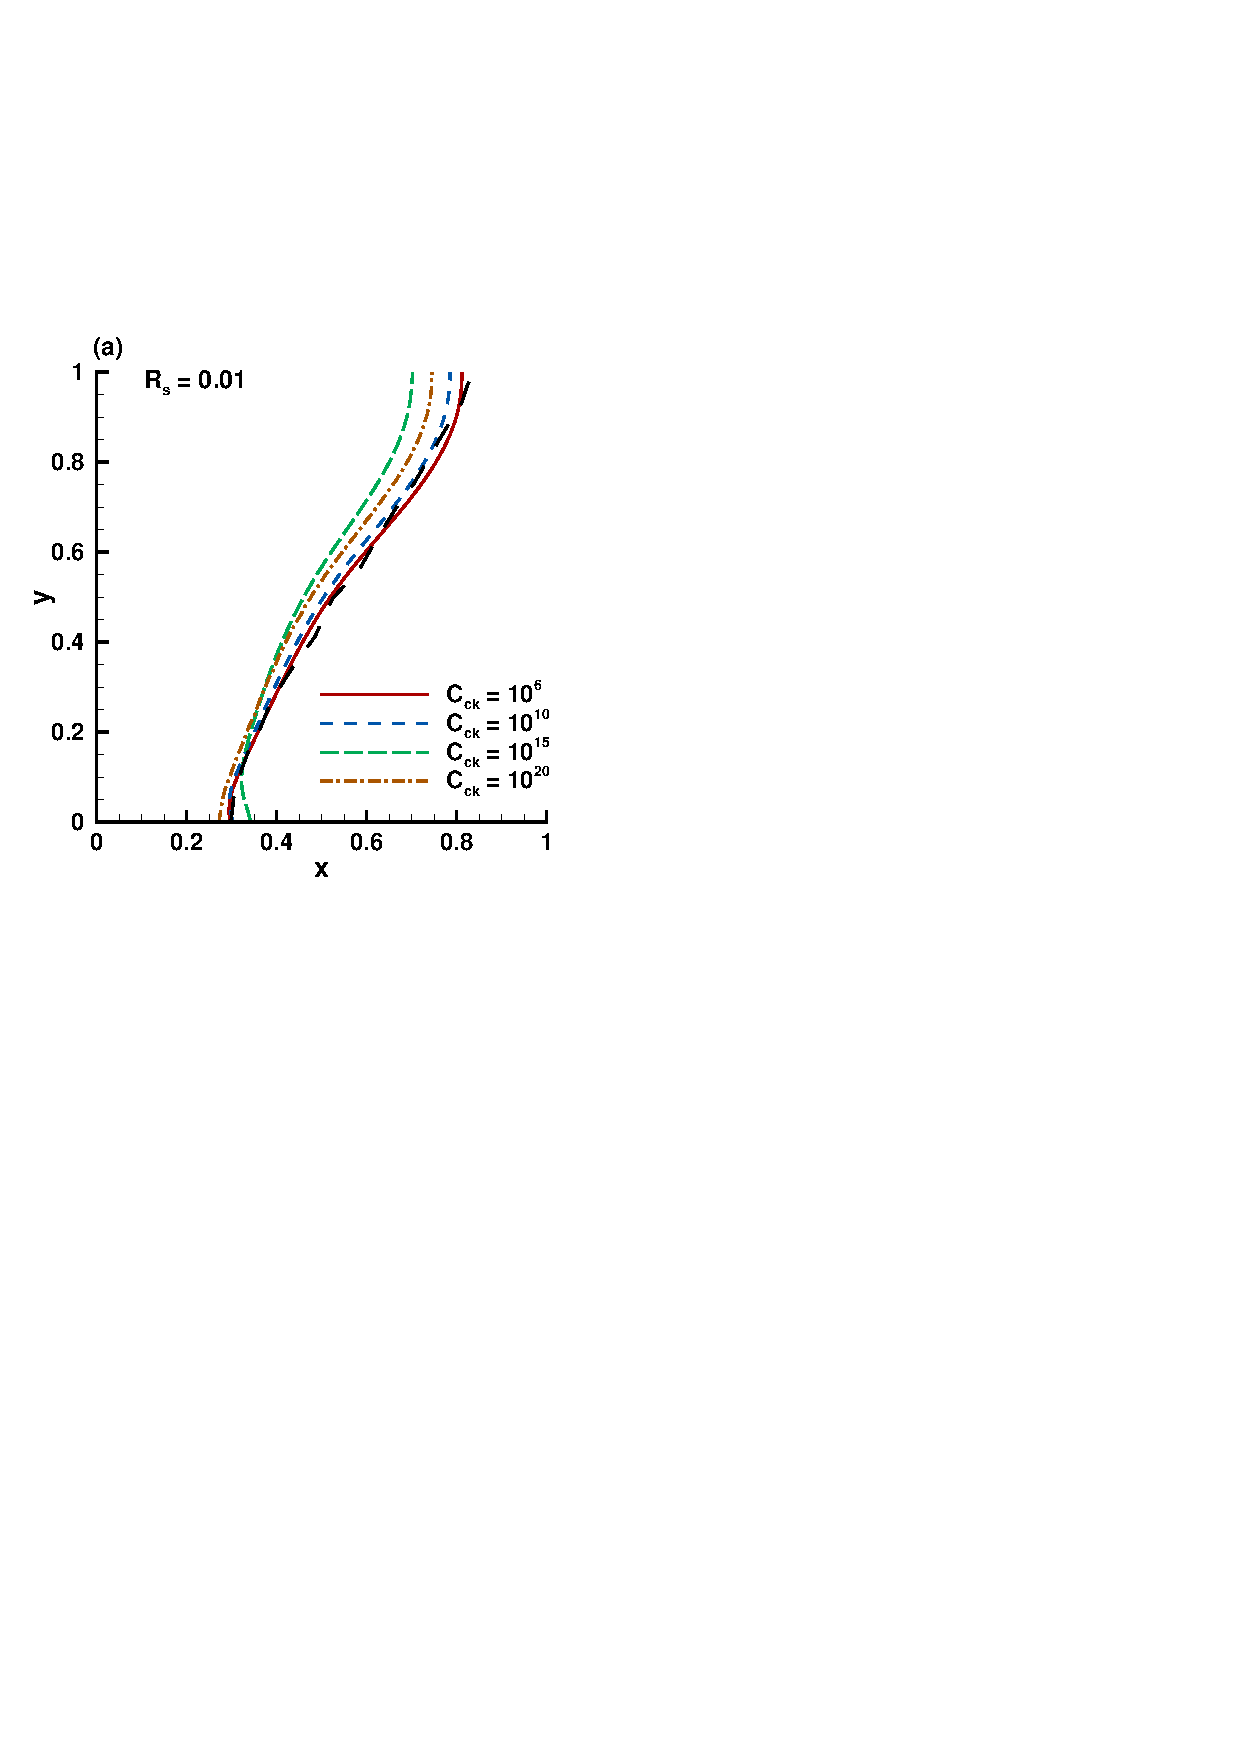
\includegraphics[width=.5\textwidth]{\figpath/Fig_cap_melting/PCM_ck_compare}
	\end{center}
	\caption{Location of the interface during the melting of the PCM using different value of $\CKC$ ranging from $10^6$ to $10^20$. Comparison with experimental data of \cite{Okada1984}}
	\label{fig:pcm-CK}
\end{figure}

\subsection{Mesh adaptativity}
The use of mesh adaptation proved mandatory in the simulation of the melting of a PCM to obtain accurate results within reasonable computational time.
For the melting case, we used five metrics intersection to adapt the mesh, based on $S^{n+1}, S^{n}, T^{n+1}, T^{n}, \vec{u}^{n+1}$. To reduce the impact of the interpolation on the global accuracy for time-depending problems, we consider the metrics computed from actual (at $t_{n+1}$) and  previous (at $t_{n}$) values, for the same variable used for adaptivity (see also \cite{Belhamadia2004_S}).
The anisotropy of the mesh is a parameter of the algorithm and it was set to values close to 1. This is an inevitable limitation since we also impose the minimum edge-length of triangles to avoid generating too large number of nodes.

\begin{figure}
	\begin{center}
		\includegraphics[width=\textwidth]{\figpath/Fig_cap_melting/Mesh_MELT}
	\end{center}
	\caption{Adapted mesh during PCM melting. (a) $12,000$ triangles: mesh is refined around the melting front and the boundary layers. (b) zoom showing the decrease of the mesh size around the temperature isoline $\theta = 0$.}
	\label{fig:pcm-mesh}
\end{figure}

The method is able to accurately capture the liquid-solid interface during the melting process and the two solidification fronts appearing during the solidification of the PCM. 
Mesh adaptivity is performed at each time step and offers a refined discretization of the regularization region where sharp gradients have to be accurately captured.  
Fig. \ref{fig:pcm-mesh}a illustrates the adapted mesh during the melting.
The mesh is refined around the melting front (Fig \ref{fig:pcm-mesh}b), localized by the temperature $\theta = 0$, while coarser mesh is applied in the solid region.
The number of triangles for the melting case is $N_t=12,000$. Non-adapted grids offering the same spatial resolution everywhere inside the computational domain would have resulted for the two cases in $N_t=9.94 \cdot 10^{10}$ triangles, respectively. Consequently, mesh adaptivity greatly helps in reducing the computational time. 

The minimum and the maximum edge-length of triangles are imposed to avoid too large meshes.
At the same time, the minimum size of triangles should allow to capture the boundary layers and the artificial mushy zone where discontinuous variables are smoothly regularized.
As far as the boundary layers are concerned, Fig. \ref{fig:min-size-bnd} draws the thermal ($\delta_T$) and the viscous ($\delta_\nu$) boundary layers, function of Prandtl number.
The scale for the thermal boundary layer in natural convection flow along a vertical wall is indeed given by \citep{bejan2013convection}:
\begin{equation} \label{eq-bnd-layer-T}
   \delta_T \sim \left\{
   \begin{array}{ll}
   H Ra^{-1/4} &	 \mbox{if }  Pr \gg 1,\\
   H Pr^{-1/4} Ra^{-1/4} &   \mbox{if } Pr \ll 1,
   \end{array}
   \right.
\end{equation}
and the scale for the thickness of the viscous boundary layer near the wall is:
\begin{equation} \label{eq-bnd-layer-nu}
   \delta_\nu \sim Pr^{1/2} \delta_T.
\end{equation}
Thus, for high-Prandtl simulations the thickness of the thermal boundary layer is thinner than the velocity and the viscous boundary layers. 
For Rayleigh numbers in the range of $10^6$ to $10^8$ and a Prandtl number of order of $50$, we have a dimensionless thickness of the thermal boundary layer of $\delta_\theta \sim 0.01$.
Conversely, for low-Prandtl simulations the viscous boundary layer is thinner than the thermal boundary layer.
For the same range of Rayleigh numbers ($10^6$ to $10^8$) and Prandtl number of order of $0.1$, we have a dimensionless thickness of the viscous boundary layer of $\delta_\nu \sim 0.015$.
Therefore the minimum edge-length must be lower than $0.01$.
Moreover, a minimum of 8 triangles should be included in the mushy zone to ensure an accurate location of the melting interface and a correct resolution of gradients.
Consequently, for all subsequent simulations the minimum edge-length is set to $h_{min} = 10^{-3}$ and the maximum edge-lenght to $h_{max} = 0.1$.

\begin{figure}
	\begin{center}
		\includegraphics[width=.8\textwidth]{\figpath/Fig_cap_melting/thermal_bnd}
	\end{center}
	\caption{Thermal and viscous boundary layer thickness function of the Prandtl number \citep{bejan2013convection}.}
	\label{fig:min-size-bnd}
\end{figure}

\subsection{Initialization}
The initialization is critical task in the Newton algorithm.
The PCM is initially solid and the temperature should be set to a cold temperature $\theta_c$ under the temperature of fusion $\theta_f$.
However, increasing abruptly the boundary temperature to a hot temperature $\theta_h$, over the temperature of fusion, in order to initiate the melting process is numerically complicate because of the strong temperature gradient between the wall and the PCM.

A first solution is to set a very thin fluid layer of  $\delta x = 0.01$ with a constant temperature $\theta = \theta_c$.
The drawback of this approach is that it is not physical and the evaluation of some physical properties depending on the temperature gradient at the heated wall, like the Nusselt number or the accumulated heat input, can be distorted.

A second approach consist of setting an establishment regime.
The temperature is increased smoothly over a small time steps combined with Rayleigh continuation steps.
This approach has physical significance and is more robust when higher Rayleigh number simulations are tackled.

\newpage

%\section{Melting of octadecane PCM: numerical validation and physical analysis}\label{sec: melting-2D}
\section{Melting of octadecane PCM in a square cavity with lateral heating} \label{sec: melting-2D} %: Comparison with experimental data of \cite{Okada1984}  and \cite{gong2015numerical}, and numerical data of \cite{bertrand1999melting}.}

Three cases are investigated.
The first consists of an experimental study of the melting of the PCM in a differentially heated square cavity of height $H=1.5$ cm by \cite{Okada1984}.
The second reproduces the melting of the PCM included in a transparent building brick of height $H = 15.2$ cm, investigated experimentally and numerically by \cite{gong2015numerical}.
The last compares our results with various numerical methods, presented by \cite{bertrand1999melting}, simulating the melting of octadecane, considering a higher value of the Rayleigh number.\\
\begin{figure}
	\begin{center}
		\includegraphics[width=0.85\textwidth]{\figpath/Fig_cap_melting/fig02_2}
	\end{center}
	\caption{Location of the interface during the melting of the PCM. 
	(a) Comparison with experimental data of \cite{Okada1984} and numerical results of \cite{dan-2014-JCP} and \cite{Wang2010} for two time instants ($\tau=0.032$ and $0.063$). Benchmark 1: $\Ray = 3.27 \cdot 10^5$, $\Pr = 56.2$ and $\Ste = 0.045$
	(b) Comparison with both experiment and simulation of \cite{gong2015numerical} for five time instants  ($\tau = 0.0002$, $0.00050$, $0.00067$, $0.00125$, $0.00252$). Benchmark 2: $\Ray = 2.48 \cdot 10^8$, $\Pr = 50$ and $\Ste = 0.072$.
	}
	\label{fig:pcm-valid}
\end{figure}

We first examine the location of the interface obtained in our simulations.
The comparison with the experimental results of \cite{Okada1984} and \cite{gong2015numerical} is presented in Figure \ref{fig:pcm-valid}.
The experimental study of \cite{Okada1984} in Figure \ref{fig:pcm-valid}(a) consists of a differentially heated square cavity of dimensions $1.5$ cm $\times \, 1.5$ cm, filled with an octadecane paraffin. The non-dimensional parameters are: $\Ray = 3.27 \cdot 10^5$, $\Pr = 56.2$ and $\Ste = 0.045$ (Benchmark 1).

For two particular time instants ($\tau=0.032$ and $\tau=0.063$), we could compare our results to available experimental \citep{Okada1984} and numerical \citep{Okada1984,Wang2010,dan-2014-JCP} data. 
In the experimental set up of \cite{Okada1984}, the author has reported that the top of the PCM was not perfectly insulated and consequently the growth of the experimental upper melting front was delayed.
In Figure \ref{fig:pcm-valid}(a), for the two time instants $\tau=0.032$ and $\tau=0.063$, the current work agrees well with the experimental results of \citep{Okada1984} at the bottom part of the melting front.
However, our results overestimate the location of the front in the top part of the cavity, which could be related to the experimental heat loss mentioned by the author.
Moreover, our results are qualitatively in a better agreement with experimental data than previously published numerical results. 
This is a direct consequence of the precise tracking of the melting front achieved by the mesh adaptivity performed at each time step. 

Figure \ref{fig:pcm-valid}(b) illustrates the interface location in the experiment and simulations of   \cite{gong2015numerical}, who studied the melting of an octadecane PCM inside a transparent building brick of dimensions 
$15.2$cm$\times 3$cm.
Their numerical simulation has been performed using a Lattice Boltzmann method. 
The non-dimensional parameters were: $\Ray = 2.48 \cdot 10^8$, $\Pr = 50$ and $\Ste = 0.072$ (Benchmark 2).
The difficulty here compared to the first validation case is the presence of a stronger natural convection flow in the fluid due to the high value of the Rayleigh number.
The location of the interface is compared for five particular time instants: $\tau = 0.0002$, $0.00050$, $0.00067$, $0.00125$ and $0.00252$.
We notice a very good agreement with the numerical and the experimental data of \cite{gong2015numerical}.


A last validation case is also investigated to test the robustness of the method.
The physical parameters are: $\Ray = 10^8$, $\Pr = 50$ and $\Ste = 0.1$ (Benchmark 3).
\cite{bertrand1999melting} compiled results provided by five different authors (Lacroix, Le Qu{\'e}r{\'e}, Gobin-Vieira, Delannoy and Binnet-Lacroix). Results provided by these authors will be hereafter referred to as (say) 'Lacroix, from \cite{bertrand1999melting}'.
They have attempted a first comparison by taking several numerical methods to compute the basic configuration presented in this section. 
Two investigators among the five failed to predict the process and showed unrealistic behaviors (see Figures \ref{fig Bertran} and \ref{fig-Nu-Lf-Bertran}):
Lacroix and Delannoy seem to be insufficiently converged (Figure \ref{fig Bertran}), and Binet-Lacroix overestimates the average Nusselt number by more than $30 \%$ (Figure \ref{fig-Nu-Lf-Bertran}).
Hence, this collection of results allows us to compare our numerical method and check whether or not realistic results are obtained for complex physical configurations.\\
We further inspect the melting front, the temporal evolution of the liquid fraction $L_f$ and the Nusselt number $N\!u$ at the left wall ($x=0$), for each of the five methods presented by \cite{bertrand1999melting}.
For the liquid fraction, the initial solid state corresponds to $L_f = 0$, while  $L_f = 1$ indicates the  complete melting of the PCM. 
The average Nusselt number $N\!u$ at $x=0$ left boundary is defined as follows:
\begin{equation}\label{eq-Nu}
N\!u = \int_{0}^1 \left(\frac{\partial \theta}{\partial x}\right)_{x=0}\, dy.
\end{equation}
\\
\begin{figure}
	\begin{center}
		\begin{minipage}[t]{0.75\textwidth}
			\includegraphics[width=\textwidth]{\figpath/Fig_cap_melting/fig03}
		\end{minipage}
	\end{center}
	\caption{Melting of a PCM (Benchmark 3). Location of the solid-liquid interface at dimensionless time (panels a to d) $\tau = 0.0005$,  $\tau = 0.002$, $\tau = 0.006$ and $\tau = 0.01$, compared with five simulations presented by \cite{bertrand1999melting}. 
	$\Ray = 2 \cdot 10^8$, $\Pr = 50$ and $\Ste = 0.1$.} \label{fig Bertran}
\end{figure}
\begin{figure}
	\begin{center}
		\begin{minipage}[t]{0.75\textwidth}
			\includegraphics[width=\textwidth]{\figpath/Fig_cap_melting/fig04}
		\end{minipage}
	\end{center}
	\caption{Time evolution of the Nusselt number (a) and the liquid fraction (b) compared with five simulations presented by \cite{bertrand1999melting}.
	$\Ray = 2 \cdot 10^8$, $\Pr = 50$ and $\Ste = 0.1$.} \label{fig-Nu-Lf-Bertran}
\end{figure}
The phase-change interface for four time steps, $\tau = 5 \cdot 10^{-4}$, $\tau = 2 \cdot 10^{-3}$, $\tau = 6 \cdot 10^{-3}$ and $\tau = 1 \cdot 10^{-2}$ is represented in Figure \ref{fig Bertran}.
Our results are for each case in fairly good agreement with those of Gobin and those of  Le Qu{\'e}r{\'e}.
Gobin uses a front-tracking method using a coordinate transformation with a finite volume method with a $62 \times 42$ grids.
Le Qu�r� solves a single domain model using a second order scheme with a finite volume method with a $192 \times 192$ grids  (\cite{gobin2000melting}).\\
The time evolution of the Nusselt number and the liquid fraction are presented in Figure \ref{fig-Nu-Lf-Bertran}.
A very good agreement is obtained with Gobin and Le Qu{\'e}r{\'e}.
A relative difference, less than $2\%$ is noticed for the Nusselt number, and a dispersion, smaller than $4 \%$, for the melted fraction.\\
The high value of the Rayleigh number $\Ray = 10^8$ results in a very demanding numerical test.
The high velocity, inducing a very narrow thermal boundary layer can lead to unrealistic results and some numerical methods have failed.
The interest of the mesh adaptation is clearly evidenced since we  initially use only $40 \times 40$ grid points.


%\section{Melting of PCM included in different geometries: cylindrical evolving inclusions, distorted mesh and rectangular}
\section{Melting of cylindrical PCM with inner heated tubes} \label{subsec-luo}

We have simulated previously phase-change problems evolving in a square cavity.
A more complex system is studied in this section, by simulating the melting of pure PCM on multitube thermal energy storage systems.
Similar configurations were studied by \cite{luo2015lattice}. Hence we could compare our numerical results to those of \cite{luo2015lattice}.
The interest is twofold: the geometry is challenging since is it complex and \cite{luo2015lattice} uses Lattice Boltzmann method, a microscopic model, which is different from previous validation cases.

Cylindrical PCM of dimensionless radius $R=1$ with tube inclusions are studied.
Shell and tube PCM are indeed most intensely used in latent heat energy storage systems.
\cite{agyenim2010review} pointed out, in a critical review of materials used for heat storage, that more than $70\%$ of the PCM container are using the shell and the tube system.
We simulate three cases taking into account one heated tube, four heated tubes, and nine heated tubes with the same contact area.
For the one heated tube case, the radius $R_i$ of the inner tube is one-quarter of the outer tube ($R_i = R/4$), for four heated tubes $R_i = R/8$ and for nine heated tubes $R_i = R/12$.
A Dirichlet boundary condition is applied to inner tubes $\theta = \theta_h$,
and a Neumann boundary condition $\frac{\partial \theta}{\partial n} = 0 $ is used at the outers.
An homogenous Dirichlet boundary condition ($\vec u = 0$) is applied everywhere for the velocity.
Only the half of the domain is simulated since the problem is symmetric.
The mesh is refined initially around inner tubes, and is dynamically adapted at each time step around the melting front and the thermal boundary layer area.
The physical parameters of the simulation are:  $\Ray = 5 \cdot 10^4$, $\Pr =0.2$ and $\Ste = 0.02$.
%The same metrics presented in \ref{sec-case1} are used for the mesh adaptation process.

The melting front (black line), the temporal evolution of the temperature field, and the time evolution of the liquid fraction, showing the effect of the configuration, are shown in Figures \ref{fig-Luo-Field} and \ref{fig-Lf-Luo}.
The configuration of the obstacles in the liquid phase, influences directly the fluid motion and the shape of melting front.
The more the number of inner tubes, the stronger the natural convection in the melted PCM.
Consequently the shape of the interface is impacted.
The heat transfer is hence enhanced, inducing a faster melting time: a ratio of $5.4$ is noticed from the melting time with nine and one tubes.

The evolution of the liquid fraction is compared with the numerical result of \cite{luo2015lattice} in Figure \ref{fig-Lf-Luo} and a good agreement is obtained.

\begin{figure}
	\begin{center}
		\begin{minipage}[t]{0.8\textwidth}
			\includegraphics[width=\textwidth]{\figpath/Fig_cap_melting/MELT_Luo_Field}
		\end{minipage}
	\end{center}
	\caption{Temperature field for the melting of cylindrical PCM, in the half of the domain, with one (a), four (b), and nine (c) heated tubes.  
	$R_i = R/4$ for one heated tube, $R_i = R/8$ for four tubes and $R_i = R/12$ for nine tubes.
	Melting  front are localized with black lines.  $\Ray = 5 \cdot 10^4$, $\Pr =0.2$ and $\Ste = 0.02$.} \label{fig-Luo-Field}
\end{figure}

\begin{figure}
	\begin{center}
		\begin{minipage}[t]{0.5\textwidth}
			\includegraphics[width=\textwidth]{\figpath/Fig_cap_melting/Lf_Luo}
		\end{minipage}
	\end{center}
	\caption{Time evolution of the liquid fraction for one, four, and nine heated tubes. Comparison with numerical results of \cite{luo2015lattice}. $\Ray = 5 \cdot 10^4$, $\Pr =0.2$ and $\Ste = 0.02$.} \label{fig-Lf-Luo}
\end{figure}

\section{Solid crust formation in a highly distorted mesh}

The solid crust formation inside a highly distorted domain, simulated by \cite{nourgaliev2016fully} is of interest in this section.
\cite{nourgaliev2016fully} used finite element with discontinuous Galerkin method.

The fluid is initially motionless with an initial dimensionless temperature $\theta_i = 2$.
The temperature of fusion is set to $\theta_f = 1.4$ according to \cite{nourgaliev2016fully} parameters.
It is worth noting that \cite{nourgaliev2016fully} have used $T_{ref} \ne T_f$ thus $\theta_f \ne 0$.

The left side is set at cold temperature $\theta_c = 1.39$ in the initial stage as the right wall was kept constant at a hot temperature $\theta_h = 2$, inducing a nearly steady-state natural circulation. 
The cold temperature at the left wall is then dropped down to $\theta_c = 1$, below the temperature of solidification starting the formation of a solid crust layer. 

\begin{figure}
	\begin{center}
		\begin{minipage}[t]{\textwidth}
			\includegraphics[width=\textwidth]{\figpath/Fig_cap_melting/Nourgaliev-Valid_2}
		\end{minipage}
	\end{center}
	\caption{Solid crust formation in a distorted mesh. Temperature field and streamlines of our simulation (a) and \cite{nourgaliev2016fully}  (b). } \label{fig-Nourgaliev}
\end{figure}

The temperature field and the streamlines are reported in Figure \ref{fig-Nourgaliev}.
We are qualitatively in a fairly good agreement with \cite{nourgaliev2016fully}.



\section{Melting of Gallium in a rectangular cavity}

The observation on the melting of the gallium in a rectangular cavity was a controversy since the question if  the flow in the fluid is monocellular of multicellular was raised by \cite{dantzig1989modelling}.
The experimental result exhibits indeed a monocellular structure, while many researchers claim this observation to be incorrect.
Prior to \cite{dantzig1989modelling} note, both experimental and numerical result support a single cell solution in the fluid phase.
Later, simulations provides solutions with multicellular flow. 
\cite{hannoun2003resolving} concluded that monocellular observation is caused by a problem of convergence of the numerical solution. It can be due to the grid size or inconsistencies in the mathematical model.

Therefore, this test case simulating the melting of the Gallium is a relevant exercice to test the consistency of our method.
To capture the very small cell during the first step of the melting, \cite{hannoun2003resolving} uses a $800 \times 1,120$ fixed grids in a rectangular domain of dimensions $6.35$ cm $\times \, 8.89$ cm. 
However, a maximum of $6 000$ triangles are necessary with our adaptive method to reproduce the numerical result of \cite{hannoun2003resolving}, that is a ratio of $10^2$.

\begin{figure}
	\begin{center}
		\begin{minipage}[t]{\textwidth}
			\includegraphics[width=\textwidth]{\figpath/Fig_cap_melting/evol_Gallium_FIELD}
		\end{minipage}
	\end{center}
	\caption{Melting of gallium: temperature field, streamlines, and melting front. 
	Physical time instants (panels a to g): $20 s$, $32s$, $36s$, $42s$, $85s$, $155s$, and $280s$.} \label{fig-Gallium}
\end{figure}

The time evolution of the flow is presented in the Figure \ref{fig-Gallium} with the plot of the streamlines for several physical times: $t_{\varphi} = 20s$, $32s$, $36s$, $42s$, $85s$, $155s$ and $280s$.
These times was voluntarily chosen for they correspond to roll merging.
\cite{hannoun2003resolving}, \cite{cerimele2002numerical} and \cite{giangi2000melting} compare the number of rolls in the fluid flow as a validation criterion.
Five primary cells are captured at $t=32s$ and decreases later through a process of roll merging as it is noticed by \cite{hannoun2003resolving}.
Our numerical results are in good agreement with the observations of \cite{hannoun2003resolving}, \cite{cerimele2002numerical} and \cite{giangi2000melting}.



\graphicspath{{\figpath/Fig_cap_solidif}}
%%%%%%%%%%%%%%%%%%don't forget if needed %%%%%%%%%%%%%%%%%%%%%
%\section[toc version]{title version%
%              \sectionmark{head version}}
%\sectionmark{head version}
%%%%%%%%%%%%%%%%%%%%%%%%%%%%%%%%%%%%%%%%%%%%%%%%%%%%%%%%%%%%%%
\def\titcourt{Numerical simulation of melting of phase change materials heated from below}
\def\titlong{Numerical simulation of melting of phase change materials heated from below}
%%%%%%%%%%%%%%%%%%%%%%%%%%%%%%%%%%%%%%%%%%%%%%%%%%%%%%%%%%%%%%%%
\chapter[\titlong]{\titlong%
              \chaptermark{\titcourt}}
\chaptermark{\titcourt}
\label{chap-MELTING-BELOW}
%%%%%%%%%%%%%%%%%%%%%%%%%%%%%%%%%%%%%%%%%%%%%%%%%%%%%%%%%%%%%%%%
%%%%%%%%%%%%%%%%%%%%%%%%%%%%%%%%%%%%%%%%%%%%%%%%%%%%%%%%%%%%%%%%

The melting of PCM heated from the side was presented in Sec. \ref{chap-MELTING}.
The dynamic of the melting, the identification of three regimes describing the melting process and the effect of the Rayleigh number have been discussed in detail.
In this chapter, we pay more attention to PCM heated from below.
This configuration is indeed known to be overspread in the nature or in human activities, such as geophysical flows (Earth's mantle formation, magma oceans) or heat dissipation from electronic devices.

While the melting of PCM heated from the side have attracted many consideration, the melting of PCM heated from below have received less attention.
\cite{diaz1984visualization,hale1980solid} have studied experimentally the solid-liquid interface morphology of PCM during basal heating.
\cite{gong1998flow} studied numerically the flow and heat transfer during the melting of pure n-octadecane in a rectangular cavity heated from below.
Recent numerical simulations investigate different boundary conditions such as
periodic configurations along the horizontal axis \citep{esfahani2018basal,madruga2018dynamic,favier2019rayleigh} or wavy surface in a rectangular cavity heated from below \citep{kousksou2014melting}.

 We investigate in this chapter the melting of a pure octadecane PCM in a square enclosure heated from below.
 The dynamics of the melting is fundamentally different in the basal heating case compared with the lateral heating.
 It has been observed that for this configuration natural convection develops in the form of Benard cells and
 results in a nonplanar solid-liquid interface. 
\citep{vasil2011dynamic,favier2019rayleigh} have studied the hydrodynamic instabilities at the onset of convection and compared their observation with the classical Rayleigh-B�nard \citep{chandrasekhar2013hydrodynamic} instability mechanism.
\citep{favier2019rayleigh} have focused their attention to the effect of the non-planar topography of the interface to the convection flow.
 On the other hand, \citep{gong1998flow,esfahani2018basal,madruga2018dynamic} mostly focused on global quantities such as the heat flux and the statistical properties of the interface.

The physical parameters considered are the same as presented in Sec. \ref{sec-melting}:
$\Pr = 56.2$ and $\Ste = 0.045$.
Three Rayleigh numbers are carried out: $\Ray = 3.27 \cdot 10^5$, $\Ray = 1.62 \cdot 10^6$, $\Ray = 3.27 \cdot 10^6$ to assess the influence of the size of the domain on the dynamic of the natural convection flow
as observed by \cite{madruga2018dynamic}.
The PCM is initially solid at a cold dimensionless temperature $\theta_c$ under the temperature of fusion.
The top of the wall is set at an isothermal temperature $\theta = \theta_c$, the vertical wall are adiabatic and the bottom is heated at a dimensionless temperature $\theta = \theta_h$.
 We carried out a two-dimensional numerical simulation even if 
 \cite{gau1983flow} and  \cite{gong1998flow} have noticed the existence of three-dimensional convection cells during the very first step of the melting process.
 Indeed, this three-dimensional convection cell can be neglected since the duration is very short compared with the whole melting step,
so that the two-dimensional model is realistic.
A qualitative observation of the dynamic of the natural convection flow and its impact on the melting front is first addressed.
Second, the observation of four regimes during the melting is discussed.
Finally, a comparison between the lateral and the basal heating is presented.

\section{Time evolution of the melting process} \label{sec-RB-melt-process}

The natural convection flow in the melt PCM during lateral heating exhibits convection cells deforming the solid-liquid interface (see Fig. \ref{fig:melt-field}).
The dynamic of the natural convection flow during the basal heating is fundamentally different.
It is well known that any non-planar topography can lead to a baroclinic flow at any Rayleigh number.

Fig. \ref{fig:melt-below} displays the structure of the natural convection in the melt PCM through a sequence of panels for temperature isolines and streamlines in the liquid phase.
An array of lengthening plumes (panel a to c) and counter-rotating convective cells (panel d to f)  is located in the liquid phase.
The number of convective cells and plumes increases with the Rayleigh number.
For $\Ray = 3.27 \cdot 10^5$, three equidistant plumes (Fig. \ref{fig:melt-below}a) and five convective cells (Fig. \ref{fig:melt-below}d) can be observed, while four and six plumes are observed for $\Ray = 1.62 \cdot 10^6$ and $\Ray = 3.27 \cdot 10^6$ respectively (Figs. \ref{fig:melt-below}b and \ref{fig:melt-below}c).
These observations agree well with the numerical results of \cite{gong1998flow} and \cite{madruga2018dynamic}.

The shape of the interface is directly linked to the dynamic of the plumes.
The mushroom form of the plumes results from the two symmetric counter-rotating convective cells surrounding each plumes.
We observe an anti-clockwise recirculation of the left convection cell and a clockwise recirculation of the right.
Thus, the melt is heated to the highest temperature at bottom and then floats up, reaches the phase change interface and splits into opposite directions.
The melt is cooled as it flows through the phase change interface.
It results a non-planar interface with a peak at the center of each couple of counter-rotating convective cells.
\begin{figure}
	\begin{center}
		\includegraphics[width=\textwidth]{\figpath/Fig_cap_melting_basal/T_MELT_BASAL_heating_2}
	\end{center}
	\caption{Melting of PCM heated from below: Temperature field and solid-liquid interface for different size of the domain. (a) $\Ray = 3.27 \cdot 10^5$ and $t=30$, (b)  $\Ray = 1.62 \cdot 10^6$ and $t=15$, (c) $\Ray = 3.27 \cdot 10^6$ and $t=10$.}
	\label{fig:melt-below}
\end{figure}

It is useful to introduce the effective Rayleigh and Nusselt numbers of the fluid layer, based on the height of the melting PCM, to describe the temporal evolution of the melting:

\begin{eqnarray}
	Ra_{e} &=& Ra \times \bar {\delta_H}^3, \\
	N\!u_{e} &=& N\!u \times \bar{\delta_H},
\end{eqnarray}
with $\bar{\delta_H}$ the averaged fluid height. Note that $\bar{\delta_H}$ here can be assimilated to the liquid fraction.
In the limit of vanishing $\Ste$ number, the classical no-slip Rayleigh-B�nard convection predicts a critical Rayleigh number $\Ray_c \approx 1707.76 $ \citep{chandrasekhar2013hydrodynamic} after which the first instability appears and the melting front becomes non-planar.
This critical value is increased for increasing values of $\Ste$.
In our simulations, the convective onset occurs at around $\Ray_e \approx 3 \times 10^3$, which is in good agreement with the observation of \citep{esfahani2018basal,favier2019rayleigh}.

\begin{figure}
	\begin{center}
		\includegraphics[width=\textwidth]{\figpath/Fig_cap_melting_basal/T_evol_Ra-327e5}
	\end{center}
	\caption{Melting of PCM heated from below: Temperature field and solid-liquid interface for different size of the domain. (a) $\Ray = 3.27 \cdot 10^5$ and $t=30$, (b)  $\Ray = 1.62 \cdot 10^6$ and $t=15$, (c) $\Ray = 3.27 \cdot 10^6$ and $t=10$.}
	\label{fig:T-evol-Ra-3.27e5}
\end{figure}

The time evolution of the melting for $\Ray = 3.27 \times 10^5$ is illustrated in details in Fig. \ref{fig:T-evol-Ra-3.27e5} in panels (a) to (f).
Before the first instability arise, the melt layer evolves solely by conduction. 
There is no noticeable fluid flow and the melting front remains straight (panel (a)).
The convective onset occurs at around $\Ray_e \approx 3 \times 10^3$ and the phase-change interface becomes non-planar (panel (b)).
The appearance of convection is marked by a change in the shape of the interface from straight to nearly periodic curve.
While the fluid depth increases, the effective Rayleigh number increases and the convective rolls are stretched vertically (panels (b) and (c)).
We note that during this stage, the number of rolls is time-independent.
This stage can be compared to the steady convection after the onset in the Rayleigh-B�nard system.
After the rolls are elongated vertically, they start to oscillate laterally and then merge to create greater rolls (panels (d) and (e)).
The essential consequence of the foregoing observation is that the melting front is modified.
The interface is actually shaped by the new flow pattern. 
Two peaks are observed but is still periodic at the interface related to the four convective rolls.
The foregoing steady convection observation is then observed again after the rolls have merged (panel (f)).

\begin{figure}
	\begin{center}
		\includegraphics[width=\textwidth]{\figpath/Fig_cap_melting_basal/T_evol_327e6_1}
		\includegraphics[width=\textwidth]{\figpath/Fig_cap_melting_basal/T_evol_327e6_2}
	\end{center}
	\caption{Melting of PCM heated from below: Temperature field and solid-liquid interface for different size of the domain.$\Ray = 3.27 \cdot 10^6$}
	\label{fig:T-evol-Ra-3.27e6}
\end{figure}

Fig. \ref{fig:T-evol-Ra-3.27e6} shows the dynamic of the melting for higher $\Ray$ number.
The size of the cavity is increased of an order of three, corresponding to $\Ray = 3.27 \times 10^6$ while the $\Ste$ number remains the same.
The stages described previously are recovered in panels (a) to (d).
At $\Ray_e = 4 \times 10^5$ the interface loses periodicity and becomes smoother without cusps (panels (e) and (f)).


\begin{figure}
	\begin{center}
		\includegraphics[width=\textwidth]{\figpath/Fig_cap_melting_basal/T_evol_654e6_1}
		\includegraphics[width=\textwidth]{\figpath/Fig_cap_melting_basal/T_evol_654e6_2}
	\end{center}
	\caption{Melting of PCM heated from below: Temperature field and solid-liquid interface for different size of the domain. (a) $\Ray = 3.27 \cdot 10^5$ and $t=30$, (b)  $\Ray = 1.62 \cdot 10^6$ and $t=15$, (c) $\Ray = 3.27 \cdot 10^6$ and $t=10$.}
	\label{fig:T-evol-Ra-6.54e6}
\end{figure}

\section{Scaling analysis} \label{sec-RB-scal-analysis}

The previous observation can be assessed more quantitatively by evaluating the heat transfert rate during the melting.
Fig. \ref{fig:NU-LF-evol}(a) plots the temporal evolution of the heat flux represented by the Nusselt number and the strength of buoyancy represented by the Rayleigh number when the melting evolve.
The onset of the convection arises at $\Ray_e = 3 \times 10^3$ when a sudden jump in $N\!u_e$ is observed.
\cite{vasil2011dynamic} have investigated a weakly non-linear stability analysis and have highlighted a superexponentional amplitude growth when the Rayleigh number becomes close to the traditional critical value in the limit of vanishing Stefan number.
This superexponential growth is moreover followed by a rapid pattern readjustment.
The trend of $N\!u_e$ at the onset of convection is in total accordance with the foregoing prediction of \cite{vasil2011dynamic}.
The results of \citep{esfahani2018basal,madruga2018dynamic,favier2019rayleigh} exhibit the same behaviour despite the different conditions (periodic lateral boundary conditions, adiabatic boundary conditions at the top of the cavity and low value of $\Pr$ for \cite{esfahani2018basal} and \cite{favier2019rayleigh}.
The rapid growth of $N\!u_e$ is followed by a power law with averaged smaller exponent $N\!u \sim \Ray^{0.28}$.
Within the framework of natural convection, the Grossmann-Lohse theory \citep{grossmann2000scaling} predicts a scaling exponent of $2/7$ for $10^5 \leq \Ray \leq 10^{14}$.
Our results match remarkably well with this power-law evolution of $N\!u \sim \Ray^{2/7}$.
The transition from steady pattern of the convective rolls to oscillating patterns followed by cell merging, as it is clearly shown in Figs. \ref{fig:T-evol-Ra-3.27e6}(d-f) and \ref{fig:T-evol-Ra-6.54e6}(c-f), 
is also illustrated by a decrease of $N\!u$ at $\Ray \sim 10^5$ followed by high oscillation in the temporal evolution of the heat transfert.
The power-law relation Nu-Ra is bounded in this stage by the average exponent of $1/3$.

One can introduce the following scaling for the time evolution of the liquid fraction.
\begin{equation}\label{eq:scal-Lf-RB}
	L_f(t) = \left[ \sqrt{2 \tau}^{(2-3 \beta)}+ c \Ray^\beta \tau \right]^{1/(2-3 \beta)},
\end{equation}
 with $\beta$ the exponent in the Nu-Ra power law, $c = \frac{(2-3 \beta) \gamma}{2 + \Ste}$ and $\gamma$ a constant fitted from numerical data.
The time evolution of the liquid fraction is illustrated in Fig. \ref{fig:NU-LF-evol}(b).
As expected, the purely diffusive stage displays the scaling $Lf \sim t^{1/2}$.
By replacing $\beta$ by the exponent value $2/7$ in eq. (\ref{eq:scal-Lf-RB}), we obtain $Lf \sim t^{7/8}$.



\begin{figure}
	\begin{center}
		\includegraphics[width=\textwidth]{\figpath/Fig_cap_melting_basal/NU-LF-PHYS}
	\end{center}
	\caption{Melting of PCM heated from below: Temperature field and solid-liquid interface for different size of the domain. (a) $\Ray = 3.27 \cdot 10^5$ and $t=30$, (b)  $\Ray = 1.62 \cdot 10^6$ and $t=15$, (c) $\Ray = 3.27 \cdot 10^6$ and $t=10$.}
	\label{fig:NU-LF-evol}
\end{figure}

%%%%%%%%%%%%%%%%%%don't forget if needed %%%%%%%%%%%%%%%%%%%%%
%\section[toc version]{title version%
%              \sectionmark{head version}}
%\sectionmark{head version}
%%%%%%%%%%%%%%%%%%%%%%%%%%%%%%%%%%%%%%%%%%%%%%%%%%%%%%%%%%%%%%
\def\titcourt{Melting-solidification cycle of a PCM with complete or parial melting}
\def\titlong{Melting-solidification cycle of a PCM with complete or parial melting}
%%%%%%%%%%%%%%%%%%%%%%%%%%%%%%%%%%%%%%%%%%%%%%%%%%%%%%%%%%%%%%%%
\chapter[\titlong]{\titlong%
              \chaptermark{\titcourt}}
\chaptermark{\titcourt}
\label{chap-SOLIDIFICATION}
%%%%%%%%%%%%%%%%%%%%%%%%%%%%%%%%%%%%%%%%%%%%%%%%%%%%%%%%%%%%%%%%
%%%%%%%%%%%%%%%%%%%%%%%%%%%%%%%%%%%%%%%%%%%%%%%%%%%%%%%%%%%%%%%%


\begin{figure}
	\begin{center}
		\includegraphics[width=\textwidth]{\figpath/Fig_cap_solidif/fig01_2}
	\end{center}
	\caption{Sketch of the computational domain and boundary conditions. General configuration (panel a) with isothermal ($\theta=cst.$) vertical ($x=0$ and $x=1$) walls and  adiabatic ($\partial \theta/\partial n = 0$) top and bottom walls. Configuration for the melting phase (panel b) with a hot left wall ($\theta=\theta_h > 0$) and a cold right wall ($\theta=\theta_c < 0$), followed by a solidification phase (panel c), when the temperature of the left wall is cooled to $\theta=\theta_{co} < 0$.}
	\label{fig: pcm-case}
\end{figure}

%\section{Solidification of the PCM}\label{sec: solidification-2D}
The fundamental operational mode of latent thermal energy storage (LTES) systems based on phase-change materials (PCM) is made of alternate melting and solidification cycles that  are not necessarily periodic. Partial melting and/or solidification of the PCM are often observed in applications and, in particular, in applications for buildings \citep{zhu2009dynamic,ascione2014energy}. 
The modern numerical approaches were mostly applied to simulate separately melting or solidification problems and only recently for alternate melting and solidification cycles \citep{wang2010numerical}. However, cyclic or periodic, melting and solidification problems have attracted considerable attention in the literature. \cite{ho1993periodic} and \cite{voller1996cyclic} studied numerically periodic melting in a square enclosure. Recently, \cite{hosseini2014experimental} presented experimental studies for the melting and the solidification of a cylindrical PCM during a charging and discharging process and \cite{chabot2017solid} studied analytically the effect of an alternate heating and cooling in a cylindrical PCM, with periodic boundary conditions. 
The present contribution is scoped  to offer an accurate numerical description of the alternate melting and solidification of a PCM.


After the melting of the PCM in Sec. \ref{chap-MELTING}, we present in this chapter the simulation of the solidification process.
The solidification of an octadecane PCM in a square cavity is considered.

\section{Numerical configuration and Non-dimensional parameter setting}
As emphasized previously,  the natural convection occurring in the melting PCM is driven by the temperature difference $\delta T = T_h - T_f$. The dimensionless number that depicts the ratio between the forces creating and those refraining motion, is the Rayleigh number, which appears in the dimensionless form of the Navier-Stokes equations with Boussinesq approximation (sec. \ref{chap-NSB}, eq. \ref{eq-Rayleigh}). The higher is its value, the more intense is the heat transfer.
Conversely, during the solidification, the phase-change is handled by the discharged temperature $T_{co}$, where the subscript 'co' stands for 'cooling'. In the geometry discussed in this chapter, this represents the temperature of the left wall. Thus, the relevant temperature difference in the solid phase of the PCM is $\delta T_{co} = T_f-T_{co}$ and the dimensionless temperature in the solid phase should be defined with respect to this $\delta T_{co}$. It is then obvious, for Eqs. (\ref{eq-Rayleigh}) and (\ref{eq-RePr}),  that the Rayleigh number should be defined using the same temperature difference.  However, because the Rayleigh number, as emphasized earlier, amounts for the motion created by hot temperature difference, we choose to keep the same definition for the Rayleigh number as for the melting case, still relevant for the melted core of the flow, where the persisting motion acts as a boundary condition for the solidification process.    
Under these conditions, in regard with the solidification process, we introduce  a new parameter,  $r_{\delta} = \delta T_{co}/(T_h-T_f)$, the normalised temperature is with respect to 
$T_f-T_{co}$ and the relevant Rayleigh number will then  $\Ray_{co}= r_{\delta} \times \Ray$, where $\Ray_{co}$ is the pseudo-Rayleigh number for solidification with a melted boundary. 
In the following, we will  describe  the process of solidification using three different values of $r_{\delta}$. 
A new scaling is moreover introduced: 
\begin{eqnarray}\label{ref-adimPCM2}
V_{ref}&=&\frac{\alpha_l}{H}  \, \Rightarrow  \, t = t_{\varphi} \frac{\, \nu_l }{ H^2 \, \Pr \,}\, \Rightarrow  \, \Rey  = \frac{1}{\Pr}.  \label{ref-adimdT} 
\end{eqnarray}
The solidification stage is indeed a slower process compared to the melting, therefore the use of an adapted scaling is more relevant.
This leads to a different time scaling for each cycle.

The sketch of the computational domain and boundary conditions are illustrated in Fig. \ref{fig: pcm-case}a, corresponding to the melting of octadecane PCM presented in Sec. \ref{sec: melting-2D}.
Starting from a melting PCM (Fig. \ref{fig: pcm-case}b), the simulation of the solidification process starts by imposing at the left-wall a constant (cold) temperature $\theta_{co}$ as it is shown in Fig. \ref{fig: pcm-case}c.
We consider two cases: \\ 
-- case CM: solidification after a Complete Melting of the material ($L_f=0.95$, Figure \ref{fig:melt-field}f) and \\
-- case PM: solidification after a Partial Melting ($L_f=0.5$, Figure \ref{fig:melt-field}d). \\
 The solid phase will propagate into the cavity from both left and right sides  (Fig. \ref{fig: pcm-case}c), which makes this case computationally challenging. The mesh adaptivity capabilities of our numerical code made possible to accurately track the 
two solidification fronts identified by the iso-line $\theta=0$.  
In the discussion below,  the solidification process starts at physical time $t_{\varphi} = 185 $ min (corresponding to $\tau=0.2$) for case CM and at $t_{\varphi} = 59$ min ($\tau=0.06$) for case PM. 

\section{Solidification after a complete melting. Case CM.} \label{sec_solid_full} 

\begin{figure}
	\begin{center}
		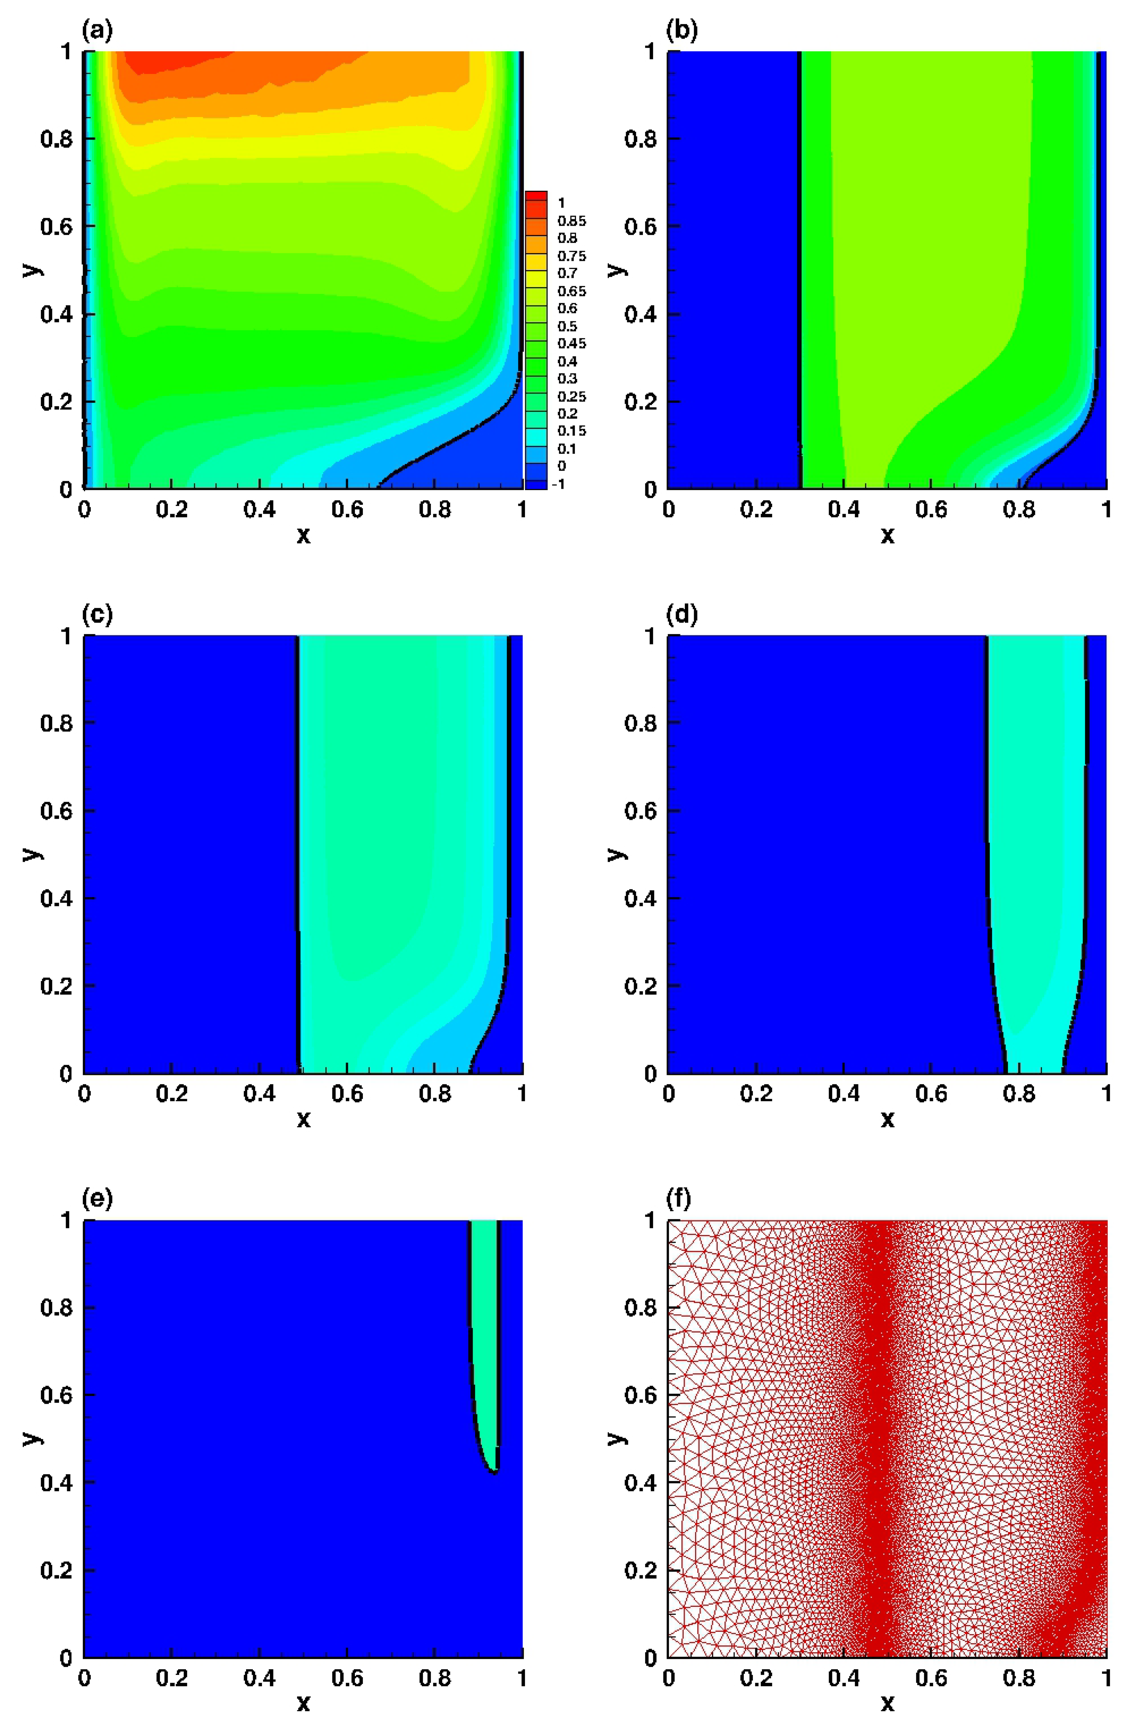
\includegraphics[width=.85\textwidth]{\figpath/Fig_cap_solidif/fig10}
	\end{center}
	\caption{Solidification of the PCM after a complete melting. 
	Temperature iso-lines in the liquid phase. 
	The solid part is represented in blue and corresponds to the region of temperature $\theta_{co} \leq \theta_f=0$. 
	Time instants (panels  a to e): $t_{\varphi} = 185$ min, $t_{\varphi} = 231$ min, $t_{\varphi} = 300$ min, $t_{\varphi} = 430$ min and $t_{\varphi} = 510$ min. 
	The adapted mesh corresponding to $t_{\varphi} = 300$ min is plotted in panel (f).  $\Ray_{co}=3.27 \cdot 10^5$. }\label{fig:evolution}
\end{figure}

The simulation continues from the state corresponding to Figure  \ref{fig:melt-field} at $t_{\varphi} =185$ min ($\tau=0.063$) and solidification follows after a complete melting. 
 Figure \ref{fig:evolution} shows the evolution of the PCM during the solidification process. At  $t_{\varphi}  =185$ min     (Figure \ref{fig:evolution}a), the liquid fraction is $L_f=0.95$ and the melting/solidification front is close to the right wall of the cavity. Setting a low temperature $\theta_{co} = -1$ at the left wall, while the right wall is maintained at a constant temperature ($\theta_{right} = -0.01 \leq \theta_f$) triggers the formation of a second solidification front, propagating from the left side of the domain. 
Figures \ref{fig:evolution}b and \ref{fig:evolution}c illustrate the left part of the cavity solidifying at a faster rate because of the very low temperature imposed at the left wall, inducing a non symmetric evolution of the solid-liquid interfaces.
The solid part is represented in blue and corresponds to the region of temperature $\theta \leq 0$.
The signature of the conductive heat transfer is characterized by the vertical shape of the left front.
Inside the liquid, the initial convection cells facilitate the heat transfer from the boundaries, resulting in a very rapid decrease of the fluid temperature. 
Temperature gradients being smoothed out during this first stage, the influence of the convection inside the liquid region is considerably reduced. As a result, the velocity inside the liquid is reduced to very low values. 
From $t_{\varphi} = 430$ min (Figure \ref{fig:evolution}d), the shape of both interfaces is almost symmetrical. 
This is a signature of a conduction dominated process. 
At $t_{\varphi} = 510$ min (Figure \ref{fig:evolution}e) the liquid region starts to shrink at the bottom side of the cavity. This process is accelerated and finally the liquid is trapped in a thin pocket and disappears completely through the top of the cavity (Figure \ref{fig:evolution}e). The complete solidification ends at $t_{\varphi} = 530$ min, \ie the liquid fraction is $L_f=0$.  
The adapted mesh, refined along the two solidification fronts, at $t_{\varphi} = 300$ min is reported in Figure \ref{fig:evolution}f, illustrating the efficiency of the adaptive mesh tool.


\section{Solidification after a partial melting. Case PM.} \label{sec_solid_partial} 

In this case, the solidification starts from the state corresponding to Figure \ref{fig:evolution_t80}a at $t_{\varphi} = 59$ min ($\tau=0.032$), when the liquid fraction is $L_f = 0.5$. 
The temperature of the left wall is suddenly lower at $\theta_{co}=-1$ as in the previous solidification simulation.  
The time evolution of the process is illustrated in Figures \ref{fig:evolution_t80}a-e, while the adapted mesh corresponding to $t_{\varphi} = 90$ min is plotted in Figure \ref{fig:evolution_t80}f. 
As in the previous case, a second  solidification front starts to propagate from the left side of the cavity. 
The straight shape of the left solid front is always observed while the right solid front is impacted by the convection cell present in the central liquid region (Figure \ref{fig:evolution_t80}b). 
The stronger convective effect is most likely due to the huge temperature difference that occurs over a smaller space distance (almost half of the volume is occupied by the solid state). 
This leads to stronger temperature gradients in the liquid region, and consequently to a stronger heat transfer.   
The two fronts merge to form a pocket of fluid which is connected to the top of the cavity (Figure \ref{fig:evolution_t80}c-e). 
It is interesting to  note that, as in the previous solidification case, the left part is solidifying at a faster rate, hence the pocket of melted PCM disappears completely from the right at the top side of the cavity (Figures \ref{fig:evolution_t80}c-e).
\begin{figure}
	\begin{center}
		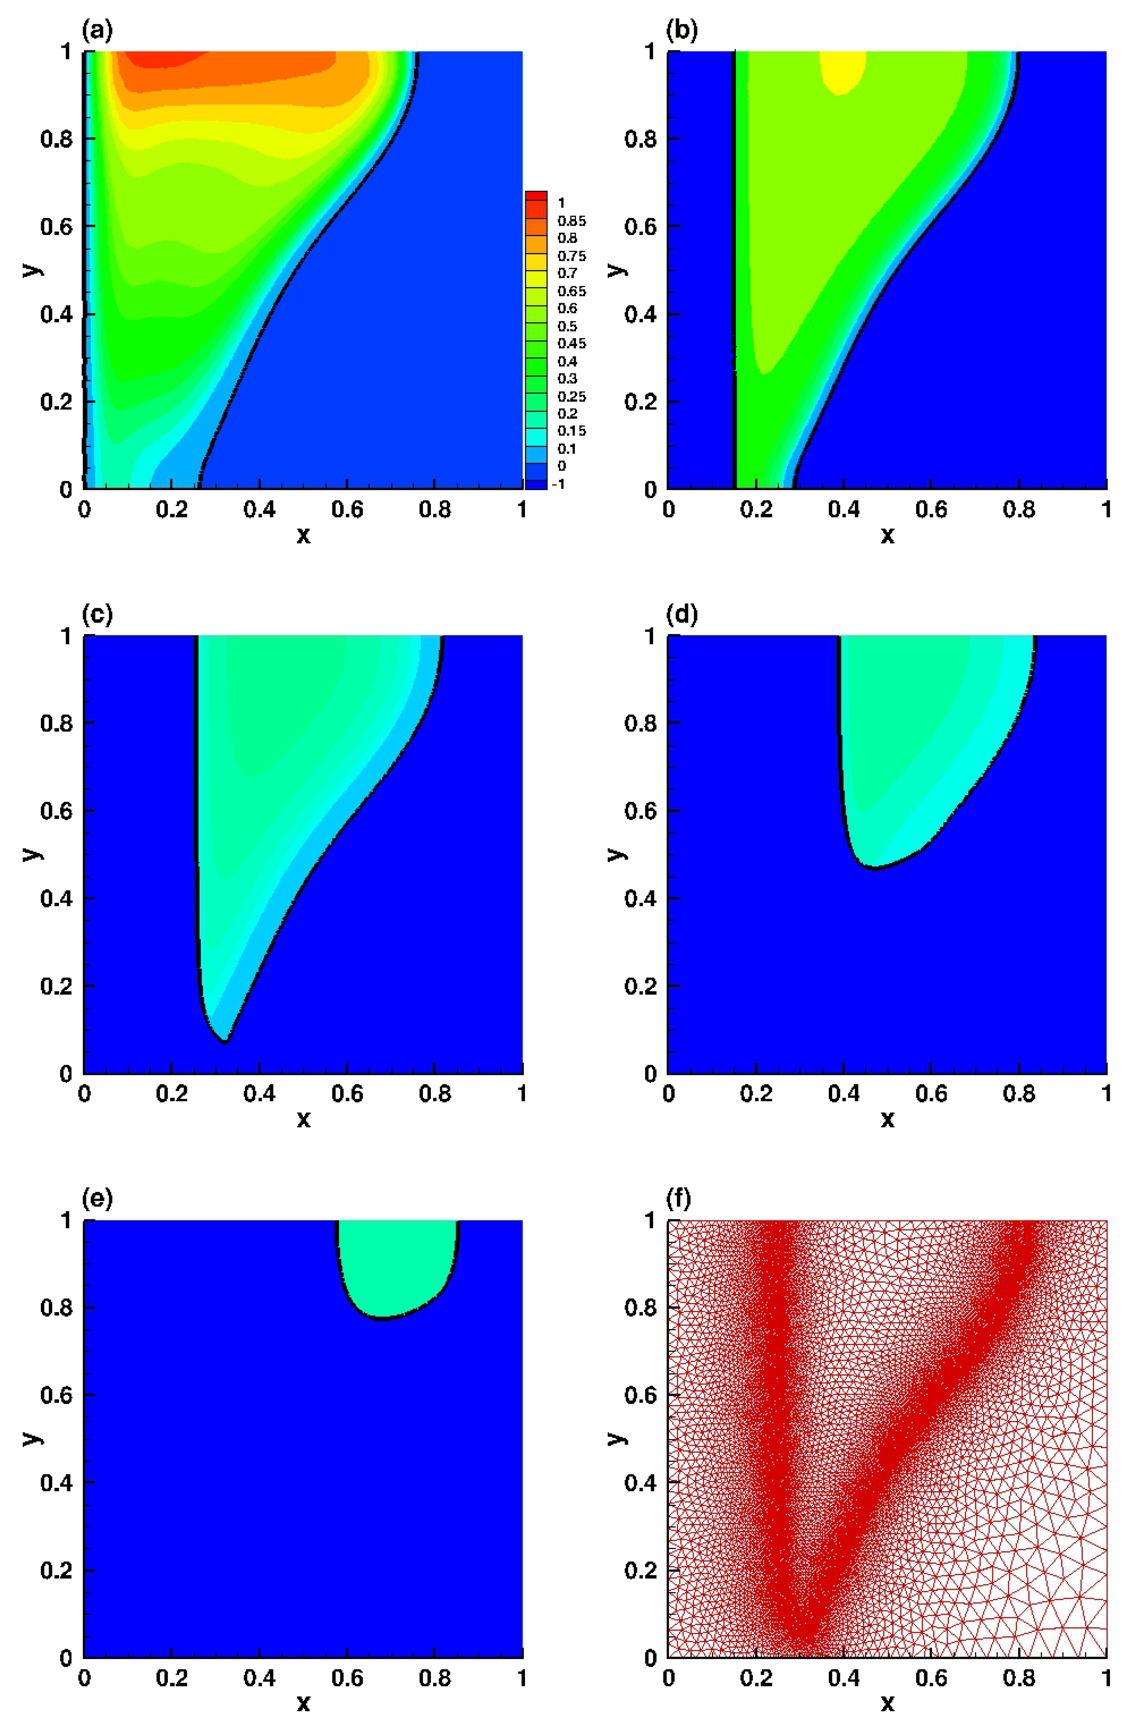
\includegraphics[width=.85\textwidth]{\figpath/Fig_cap_solidif/fig11}
	\end{center}
	\caption{Solidification of the PCM after a partial melting. Temperature iso-lines in the liquid phase. The solid part is represented in blue and corresponds to the region of temperature $\theta_{co} \leq \theta_f=0$. Time instants (panels  a to e): $t_{\varphi} = 59$ min, $t_{\varphi} = 70$ min, $t_{\varphi} = 90$ min, $t_{\varphi} = 131$ min and $t_{\varphi} = 200$ min. The adapted mesh corresponding to $t_{\varphi} = 90$ min is plotted in panel (f).  $ \Ray_{co}=3.27 \cdot 10^5$.}\label{fig:evolution_t80}
\end{figure}

\section{Analysis of the solidification cycle from two different initial conditions: complete and partial melting. Cases CM and PM. } \label{sec_freezing_full} 

The aim of this subsection is to investigate the temporal evolution of some physical properties of the solidification process, from two different initial conditions: i) completely melted volume (case CM) and ii) partially melted volume ($50\%$ of the fluid is melted, case PM).  
 
Figure \ref{fig:Lf_full_1D_profil} represents the temporal  evolution of the liquid fraction, note that the average Nusselt number is calculated at the cooled wall defined similarly to (\ref{eq-Nu}) but it can be negative in this case and the accumulated heat input $Q_0$, for the two investigated cases. $Q_0$ is defined as follows:
\begin{equation}
    Q_0 = \int_0^{t_{\varphi}} N\!u \, d t_{\varphi},
    \label{eq-Q0}
\end{equation}

\Blue{
Simulations for three values $r_{\delta} = 1$,  $r_{\delta} = 5$ and  $r_{\delta} = 10$ are carried out.
}

Figure \ref{fig:Lf_full_1D_profil}(a) illustrates the temporal evolution of the liquid fraction $L_f$ for the CM case. 
Complete melting occurs for $t_{\varphi} =185$ min, after which solidification starts, with a continuous decrease of $L_f$ till complete solidification is achieved. 
For the lowest value of \Blue{$r_{\delta}$, corresponding to $\Ray_{co} = 3.27 \cdot 10^5$}, the solidification process ends at $t_{\varphi} = 530$ min. 
Then, the higher value of \Blue{$r_{\delta}$}, the faster the discharge process,
with final times $t_{\varphi} = 260$ min and $t_{\varphi} = 230$ min for cases \Blue{$\Ray_{co} = 1.62 \cdot 10^6$} and \Blue{$ \Ray_{co} = 3.27 \cdot 10^6$}, i.e. a drop of the cold boundary temperature by a factor of 5 and 10 respectively.
The solidification speed, quantified by $d L_f/ d t_{\varphi}$ is  nearly constant during almost the whole process for each case.  
This uniformity of the process indicates that the natural convection flow vanishes during the solidification, and conduction remains the only heat transfer mode.   

Figure \ref{fig:Lf_full_1D_profil}(b) plots the temporal evolution of $L_f$ for the PM case. 
As previously discussed, $50\%$ of the volume is melted, at time $t_{\varphi} = 59$ min, then solidification starts. 
Furthermore, noticeable is that, despite that solidification process is started, $L_f$ continues to increase slightly at the very beginning of the discharge stage, and then decreases monotonically towards $0$ at $t_{\varphi} = 240$ min.
The heat stored in the melted PCM continues to melt the remaining solid PCM until the convection becomes negligible.
It is worth noticing that this behavior is not observed in the complete melting case because of the imposed temperature at the right wall.  


\begin{figure}[!h]
\begin{center}
\begin{minipage}[t]{0.7\textwidth}
	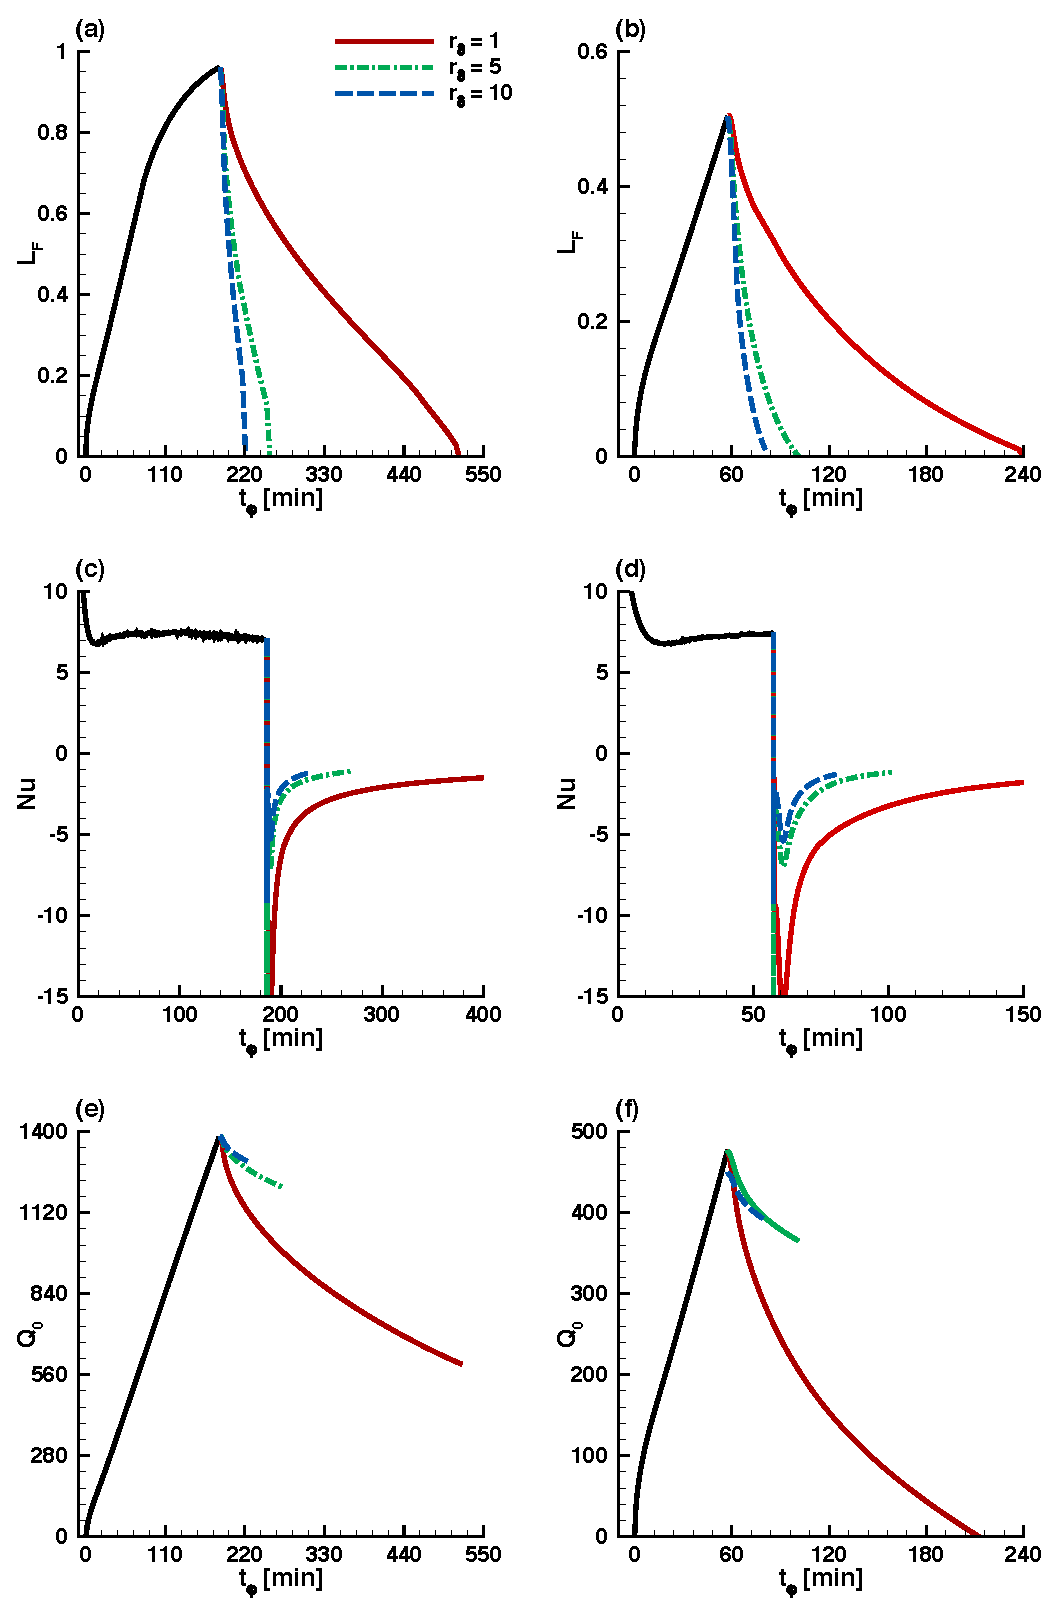
\includegraphics[width=\textwidth]{\figpath/Fig_cap_solidif/fig12_3}
\end{minipage}
\end{center}
\caption{Temporal evolution of the  liquid fraction ($L_f$), the Nusselt number $N\!u$, and the accumulated heat input $Q_0$ during the entire melting-solidification cycle. Case CM  (left) and  case PM  (right).}\label{fig:Lf_full_1D_profil}
\end{figure}

Let us now pay attention to the transfers occurring at the left wall, suddenly submitted to a lower temperature. This is done through the temporal evolution of the Nusselt number,  and the temporal-integrated values of the Nusselt number, or the accumulated heat input.     

Panels (c) and (d) of the Figure \ref{fig:Lf_full_1D_profil} illustrate the Nusselt number for the CM and PM.  
The three investigated Rayleigh numbers are shown, with clear differences between them. This difference corroborates with that already reported for the melting case, over shorter times scales.   This indicates that the heat transfer during the solidification process is fundamentally different from the melting one.

For the CM case, for \Blue{$\Ray_{co}=3.27 \cdot 10^5$,  the Nusselt number first decreases sharply, for  $t_{\varphi} \leq 18$ min, then it reaches a plateau at $N\!u=7$ during the complete melting. At $t_{\varphi}=185$ min, solidification starts and $N\!u$ suddenly decreases over very short times, reaching negative values ($N\!u\approx -15$). It follows an increase of $N\!u$ with time, up to reaching an asymptotic value close to $0$ (zero temperature gradients, i.e. uniform temperature at the left wall).  
The same mechanism is observed over a shorter time interval when} \Blue{$\Ray_{co}$} is increased.

For the PM case, the Nusselt number also decreases sharply to a negative value when the solidification starts.
However, the convection flow remaining in the melted region influences the heat transfer at the very beginning of the solidification process.
The hot fluid in the middle of the melted PCM is advected by the natural convection flow to the boundaries and induces a temperature gradient at the left wall, resulting into an oscilating behavior of the Nusselt number before reaching asymptotic value.
This is in agreement with the previous comment about the melting continuing in the right part of the cavity, despite the solidification has started, and the slight increase of the liquid fraction at the very first time steps of the discharging process.


Both charge and  discharge cycles are better illustrated in the time evolution of the accumulated heat $Q_0$ defined in (\ref{eq-Q0}), as it is shown in panels (d) and (e) of Figure  \ref{fig:Lf_full_1D_profil}.
Heat is first stored during the melting stage, corresponding to $t_{\varphi} \leq 185$ min for CM (Figure \ref{fig:Lf_full_1D_profil}(d)) and $\tau \leq 59$ min for PM (Figure \ref{fig:Lf_full_1D_profil}(e)), and is then restored during the solidification stage.

\noindent The CM case indicates higher value of $Q_0$ ($Q_0 = 1400$, for \Blue{$\Ray_{co} = 3.27 \cdot 10^5$) compared to the PM case ($Q_0 = 500$), meaning that PCM is more efficient in terms of heat storage.
However, PM case exhibits well balanced characteristic times between the solidification and the melting stages for} \Blue{$\Ray_{co} = 3.27 \cdot 10^5$.}
Besides, when the Ra number increases, the stored heat is discharged faster.

\noindent Moreover, the temperature and the velocity profiles drop sharply during the first step of the cooling process and become almost equal to zero very early in the whole domain.
This means that conduction dominates the solidification process, and the convection becomes rapidly negligible.
As a consequence, the melting fronts are vertical and have a symmetric position with respect to the center of the cavity. \\

%%%%%%%%%%%%%%%%%%don't forget if needed %%%%%%%%%%%%%%%%%%%%%
%\section[toc version]{title version%
%              \sectionmark{head version}}
%\sectionmark{head version}
%%%%%%%%%%%%%%%%%%%%%%%%%%%%%%%%%%%%%%%%%%%%%%%%%%%%%%%%%%%%%%
\def\titcourt{Numerical simulation of 3D configurations using domain decomposition method}
\def\titlong{Numerical simulation of 3D configurations using domain decomposition method}
%%%%%%%%%%%%%%%%%%%%%%%%%%%%%%%%%%%%%%%%%%%%%%%%%%%%%%%%%%%%%%%%
\chapter[\titlong]{\titlong%
              \chaptermark{\titcourt}}
\chaptermark{\titcourt}
\label{chap-3D-SIMULATION}
%%%%%%%%%%%%%%%%%%%%%%%%%%%%%%%%%%%%%%%%%%%%%%%%%%%%%%%%%%%%%%%%
%%%%%%%%%%%%%%%%%%%%%%%%%%%%%%%%%%%%%%%%%%%%%%%%%%%%%%%%%%%%%%%%

Having extensively validated and analysed 2D  melting and solidification configurations for phase-change materials in the previous chapters, we now perform parallel computing of three-dimensional liquid-solid phase-change systems involving natural convection.
We use the recent library \texttt{ffddm} that makes available in FreeFem++ state-of-the-art scalable Schwarz domain decomposition methods (DDM).
Our motivation to expand our numerical model to 3D configuration is first motivated by the lack of publications in the literature for accurate 3D simulations of phase-change materials.
%Also, since publications related to three-dimensional simulation of phase-change material is not abundant in the literature, we expand our numerical model to 3D configuration.
Also, experimental investigations against which we have validated our numerical method involve three-dimensional effects that we have assumed to be neglected in our comparisons.
The latter assumption is however not valid for high $\Ray$ numbers.

The main feature of our numerical approach is the use of 3D adaptive mesh, performed using \textit{mmg3d} library.
\textit{Mmg3d} is a 3D remeshing software developed by \cite{dobrzynski:hal-00681813}, which allows to remesh an initial mesh made of tetrahedra.
The metrics for the mesh adaptation are computed using \textit{mshmet} library, which computes anisotropic metric based on solution variations.
Since the mesh adaptivity procedure is done through a sequential algorithm, we compute the metrics with respect to the coarse mesh, then finer local meshes are then generated in parallel during the mesh decomposition step in order to reach the desired level of refinement for the subdomains.
We use \textit{Metis} library to split the domain into subdomains.
The number of layers of mesh elements in the overlap region between subdomains is set to $2$ for all subsequent simulations.
This chapter is part of the paper [G. Sadaka, A. Rakotondrandisa, F. Luddens, C. Lothod�, P-H. Tournier, I. Danaila, \textit{Parallel finite-element codes for the simulation of solid-liquid phase-change systems with natural convection}, to be submitted to CPC, 2019].

For three-dimensional applications, direct solvers used in the frame of 2D problems are not appropriate and iterative methods must be employed since memory requirements for \textit{LU} decomposition would rapidly exceed the capacity of available computers.
The linear system of equations resulting from the Newton linearisation are thus solved using parallel \textit{GMRES} Krylov method.
Since it is well known that iterative methods can suffer from convergence problems, we adapt the number of subdomain in such a way that each processor could handle $1,000$ tetrahedra.
The Optimized Restricted Additive Schwarz (ORAS) preconditioned \textit{GMRES} solver proved to be extremely efficient since an order of 30 iterations were necessary to get a residual norm of $10^{-9}$ for each Newton iteration.
We note that in all numerical simulations, a quadratic ($\PP_2$) discretization of $\theta$ was used.

The remainder of this chapter is as follows.
In Sec. \ref{sec: natconv-air-3D}, we validate the 3D natural convection of air inside differentially heated cube against numerical benchmark by \cite{Wakashima-2004}.
We also compare the solutions obtained by the parallel computation with the solution obtained using sequential algorithms.
Then, the natural convection of water is investigated in Sec. \ref{sec-3D-water-convec}. %to illustrates the capability of our method to deal with non-linear body force $f_B$ and to capture accurately interfaces, mainly the density inversion.
Finally, the lateral melting of n-octadecane PCM inside 3D enclosure is addressed.

\section{Numerical simulation of the natural convection of air in 3D configurations}\label{sec: natconv-air-3D}
 Following the same line of argument that was outlined in Chapters. \ref{chap-NATCONV} and \ref{chap-MELTING}, we start by presenting the natural convection of air, that involves linear description of the buoyancy force $f_B$, and include gradually additional non-linearities.
The well-known thermally driven cavity is addressed first in Sec. \ref{subsec-3D-natconv-air}. %and the problem is then complicated by incorporating a heated cube in the center of the domain in Sec. \ref{sub-OBSTACLE-3D}.
The physical parameters are the same than used in the 2D simulations ($\Prd = 0.71$) and we investigate three Rayleigh numbers: $\Ray=10^4$, $\Ray=10^5$, and $\Ray=10^6$. 
The walls are rigid and impermeable. The vertical walls at $x=0$ and $x=1$ are isothermal and have different temperatures $T_h = 0$ and $T_c = 1$ respectively. The remaining walls are considered adiabatic. 
The fluid is initially at rest and the temperature is linearly distributed from the cold to the hot walls.
We solve the steady Eq. \ref{eq-weak-steady} by increasing smoothly the parameter $\alpha$ before the Boussinesq term (which can be assimilated to a Rayleigh continuation step) with a maximum of $6$ steps for $\Ray = 10^6$.

\begin{figure}
\begin{minipage}{\linewidth}
\begin{center}
 {\includegraphics[width=.95\textwidth]{\figpath/Fig_cap_natconv/Validation_3D_seq_T1}}
\end{center}
\end{minipage}
\caption{3D differentially heated cavity. Temperature contours at the mid-plane of ($y=0.5$); comparison with the results of \cite{Wakashima-2004} (left images). }
\label{fig-3DT} 
\end{figure}
We first compare the current simulation with the numerical data of \cite{Wakashima-2004}, who have used a forth order finite difference method, with a vorticity-stream function formulation with different uniform meshes of  $120 \times 120 \times 120 \times 10$ grid nodes.
Our results were obtained using uniform grids of $ 40 \times 40 \times 40$.
Since the converged flow pattern and temperature distributions are symmetrical with respect to the center of the cavity for the investigated Rayleigh number,
we display in 
Fig. \ref{fig-3DT} the temperature field at the mid section ($y = 0.5$), for each of the three Rayleigh numbers $\Ray = 10^4$ (top), $\Ray = 10^5$ (middle), $\Ray = 10^6$(bottom).  
On the left we display the numerical results of \cite{Wakashima-2004} and on the right the present simulation.
The comparison with the benchmark solution exhibits a fairly good agreement with the considered test case.
The higher the Rayleigh number, the finner the thermal boundary layer thickness in the vicinity of the vertical walls.
One can also notice the stagnant fluid with stratified temperature in the center of the domain in both numerical solutions.

More accurate comparison is addressed in Tab. \ref{tab-3D-locU} between the present simulation and numerical data from the literature.
We assess the maximum velocity values and their corresponding location with benchmark solution of \cite{Wakashima-2004} and numerical results of \cite{Raluca2013}.
The solutions show a good convergence on a mesh $3$ times coarser than the one proposed by  \cite{Wakashima-2004} and an excellent agreement is found for all values of the Rayleigh number.
For $\Ray = 10^4$ the current simulation shows a relative difference of $0.15 \%$ for $u_{max}$ and $0.28 \%$ for $v_{max}$ with the latter.
Larger differences of $6.55 \%$ is found with those obtained by \cite{Raluca2013}, since their results are smaller than the considered benchmark.
However, for $\Ray = 10^5$ and $10^6$ the results are in good agreement.


\begin{table}
   \begin{center}
      \begin{tabular}{*{3}{cl}}
           & $u_{max}$ ($y$) & $v_{max} ($x$)$ \\ \toprule
           $\Ray = 10^4$ & $0.198094$ ($0.826772$) & $0.220973$ ($0.11811$) \\ 
           \cite{Wakashima-2004} & $0.1984$ ($0.8250$) & $0.2216$ ($0.1177$) \\
           \cite{Raluca2013} & $0.1859$ ($0.8230$) & $0.2234$ ($0.1172$) \\ \hline
           
           $\Ray = 10^5$ & $0.140367$ ($0.850394$) & $0.245454$ ($0.0629921$) \\ 
           \cite{Wakashima-2004} & $0.1416$ ($0.8500$) & $0.2464$ ($0.0677$) \\
           \cite{Raluca2013} & $0.1461$ ($0.8540$) & $0.2459$ ($0.0703$) \\ \hline
           
           $\Ray = 10^6$ & $0.0809247$ ($0.858268$) & $0.257719$ ($0.0393701$) \\ 
           \cite{Wakashima-2004} & $0.08111$ ($0.8603$) & $0.2583$ ($0.0323$) \\ 
           \cite{Raluca2013} & $0.0830$ ($0.8550$) & $0.2553$ ($0.03905$) \\ \bottomrule
          
           
               \end{tabular}
   \end{center}
   \caption{3D differentially heated cavity. Comparison with benchmark solutions for $\Ray = 10^4$, $\Ray = 10^5$, $\Ray = 10^6$.}
   \label{tab-3D-locU}
\end{table}

Further comparison of the the parallel solver with the sequential algorithm is offered in Tab. \ref{tab-T1} for all cases. 
\begin{table}
	\begin{center}
		\begin{tabular}{|*{6}{c|}}
			\hline
			 $\Ray$ & \em{nb proc }                  & $||u||_{2}$                        & $||u||_{\infty}$                & $||T||_{2}$              & $||T||_{\infty}$\\ \hline \hline
			\multirow{4}{*}{$10^4$} & 28 & $1.12496 \cdot 10^{-6}$ & $3.1 \cdot 10^{-6}$ & $ 3.09966 \cdot 10^{-6} $ & $7 \cdot 10^{-6}$ \\% \hline
			\cline{2-6}
			& 42 & $1.53698 \cdot 10^{-6}$ & $5.1 \cdot 10^{-6}$ & $ 3.23352 \cdot 10^{-6} $ & $8 \cdot 10^{-6}$ \\ \cline{2-6} %\hline 
			& 56 & $1.55576 \cdot 10^{-6}$ & $5.1 \cdot 10^{-6}$ & $ 3.4342 \cdot 10^{-6} $ & $8 \cdot 10^{-6}$  \\ \cline{2-6} %\hline
			& 70 & $1.25622 \cdot 10^{-6}$ & $3.6 \cdot 10^{-6}$ & $ 3.56048 \cdot 10^{-6} $ & $8 \cdot 10^{-6}$ \\ \hline \hline
			\multirow{4}{*}{$10^5$} & 28 & $1.73254 \cdot 10^{-6}$ & $6.1 \cdot 10^{-6}$ & $ 2.40467 \cdot 10^{-6} $ & $7 \cdot 10^{-6}$ \\% \hline
			\cline{2-6}
			& 42 & $2.84973 \cdot 10^{-6}$ & $7.78 \cdot 10^{-6}$ & $ 3.53003 \cdot 10^{-6} $ & $9 \cdot 10^{-6}$ \\ \cline{2-6} %\hline 
			& 56 & $3.00832 \cdot 10^{-6}$ & $7.39 \cdot 10^{-6}$ & $ 4.17769 \cdot 10^{-6} $ & $1.1 \cdot 10^{-5}$  \\ \cline{2-6} %\hline
			& 70 & $3.68118 \cdot 10^{-6}$ & $9 \cdot 10^{-6}$ & $ 4.70846 \cdot 10^{-6} $ & $1.2 \cdot 10^{-5}$ \\ \hline \hline
			\multirow{4}{*}{$10^6$} & 28 & $6.61804 \cdot 10^{-6}$ & $1.826 \cdot 10^{-5}$ & $ 3.46504\cdot 10^{-6} $ & $1.1 \cdot 10^{-5}$ \\% \hline
			\cline{2-6}
			& 42 & $5.93966 \cdot 10^{-6}$ & $1.5 \cdot 10^{-5}$ & $ 3.98082 \cdot 10^{-6} $ & $1.2 \cdot 10^{-5}$ \\ \cline{2-6} %\hline 
			& 56 & $7.05144 \cdot 10^{-6}$ & $1.9247 \cdot 10^{-5}$ & $ 5.0044 \cdot 10^{-6} $ & $2 \cdot 10^{-5}$  \\ \cline{2-6} %\hline
			& 70 & $6.02152 \cdot 10^{-6}$ & $1.68 \cdot 10^{-5}$ & $ 4.50094 \cdot 10^{-6} $ & $1.8 \cdot 10^{-5}$ \\ \hline
		\end{tabular}
	\end{center}
	\caption {3D differentially heated cavity. Comparison between sequential and ffddm algorithm for uniform grids of $40 \times 40 \times 40$ }
	\label{tab-T1}
\end{table}
We compute $L^2$ and $L^\infty$ norms of the velocity and the temperature.
The number of subdomain varies from $28$ to $70$ for $1.8$ millions of unknown to assess the consistency of our method with the number of subdomains 
The difference between both algorithm is of order of $10^{-6}$
and we do not observe a large variation of the error when the number of subdomains keep increasing.
The comparison with the sequential algorithm was limited to $40 \times 40 \times 40$ grids size since the simulations are highly demanding in CPU time.
The steady state solution required $57$ CPU hours and $3$ runs (restarts) with $120$ Go of memory for the sequential algorithm, for the highest value of the Rayleigh number. 
The computational time is considerably reduced using DDM and 3D simulations becomes affordable  since only $21$ CPU minutes  ($1308.48$ s) were necessary with $70$ processors to achieve the same case with an error of $6.02152 \cdot 10^{-6}$ on $\vec u$ and $ 4.50094 \cdot 10^{-6} $ on $\theta$.


%\subsection{Natural convection in a cube with an inner heated obstacle}\label{sub-OBSTACLE-3D}
%A heated obstacle, at constant temperature $\theta_o = 0.8$, is included in the center of the unit cube as depicted in Fig. \ref{fig-obstacle-Ra1e4}.
%The vertical walls are differentially heated with $\theta_h = 0.5$ and $\theta_c = -0.5$.
%Simulation is performed for $\Ray = 10^6$.
%
%The temperature contours at the mid-plane is displayed in Fig. \ref{fig-obstacle-Ra1e4}b.
%At the investigated Rayleigh number, the heat transfer is completely governed by convection.
%A plume, tilted to the right, towards cold wall could be observed above the hot obstacle.
%The clockwise recirculation of the fluid transport actually the heated air from the hot (center) obstacle to the cold (right) wall.
%When compared to the two-dimensional case, the flow inside the 3D cubic box is obviously more complex, since a spiral movement of the fluid occurs along the walls whereas boundary layer heat transfer takes place in the same region.
%
%We also assess The number of CPU used were chosen to satisfy the criterion degrees of freedom per CPU in the range of $50,000$ to $200,000$.
%
%
%
%
%\begin{table}
%\begin{center}
%\begin{tabular}{|*{7}{c|}}
%
%		\hline
%                $\Ray$ & \em{nbseg} & \em{nb proc }                    & $||u||_{2}$                        & $||u||_{\infty}$                & $||T||_{2}$              & $||T||_{\infty}$\\ \hline \bottomrule
%                \multirow{12}{*}{$10^6$}& \multirow{4}{*}{40} & 28 & $0.000830258$ & $0.0203142$ & $ 0.0017393 $ & $0.034896$ \\ \cline{3-7}
%                & & 42 & $0.000831142$ & $0.0203468$ & $ 0.00175767 $ & $0.034882$ \\ \cline{3-7}
%                & & 56 & $0.00085423$ & $0.0203416$ & $ 0.00181677 $ & $0.034887$ \\ \cline{3-7}
%                & & 70 & $0.00083373$ & $0.0203248$ & $ 0.00175643 $ & $0.03489$ \\ \cline{2-7}
%                & \multirow{4}{*}{60} & 112 & $0.000420192$ & $0.0023909$ & $ 0.000953569 $ & $0.01381$ \\ \cline{3-7}
%                & & 140 & $0.000416573$ & $0.002334$ & $ 0.000947099 $ & $0.013775$ \\ \cline{3-7}
%                & & 168 & $0.000405618$ & $0.002399$ & $ 0.000923159 $ & $0.013755$ \\ \cline{3-7}
%                & & 196 & $0.000412466$ & $0.0024075$ & $ 0.000945884 $ & $0.013725$ \\ \cline{2-7}
%                & \multirow{4}{*}{80} & 224 & $0$ & $0$ & $ 0 $ & $0$ \\ \cline{3-7}
%                & & 238 & $0.000109568$ & $0.0005326$ & $ 0.000215454 $ & $0.000984$ \\ \cline{3-7}
%                & & 252 & $0.000126653$ & $0.0006788$ & $ 0.000215497 $ & $0.001115$ \\ \cline{3-7}
%                & & 266 & $8.37328\cdot10^{-5}$ & $0.00034267$ & $ 0.000167761 $ & $0.000663$ \\  \toprule
%      
%\end{tabular}
%\end{center}
%\caption {3D convection in a cube with an inner heated cube. Comparison with respect to the most resolved solution ({\em nbseg} $= 80$) for $\Ray = 10^6$.}
%\label{tab-T2}
%\end{table}
%
%
%
%
%\begin{figure} [!ht]
%\begin{center}
%\begin{minipage}{\linewidth}
% {\includegraphics[width=0.98\textwidth]{\figpath/Fig_cap_natconv/3D_OBSTACLE_field_2}}
%\end{minipage}
%\end{center}
%\caption{3D convection in a cube with an inner heated cube. Temperature fields for $Ra = 10^6$.}
%\label{fig-obstacle-Ra1e4} 
%\end{figure}
%
%\clearpage
%\newpage
\section{Numerical simulation of the natural convection of water in a cube cavity.} \label{sec-3D-water-convec}

We perform the natural convection of water inside cubic cavity using adaptive mesh in this section.
The dimensionless parameters are the same that used in Chapter \ref{sec: natconv-water} ($\Ray=2.518084\cdot 10^{6}$ and $\Prd=6.99$).
We impose cold dimensionless temperature $\theta_c = 0$ at $x=1$ (right wall), hot temperature $\theta_h = 1$ at $x=0$ (left wall), and a homogeneous Neumann boundary condition at the remaining walls.
Dirichlet boundary condition $\vec u = 0$ is prescribed over the whole $\partial \Omega$.
In view of anomalous thermal variation of water density, we adapt the mesh along $\theta = 0.4$ to capture correctly the flow structure.
The main limitation of 3D simulations of water convection in the literature is indeed the size of the mesh resolution when fixed grid models are used.
As an example, \cite{Giangi-2000} and \cite{Kowalewski-2003}  have investigated a mesh sensitivity analysis, and have concluded that even by using $81^3$ grid points, the variation of the velocity was still significant,
and beyond such mesh resolution, the problem becomes computationally expensive. %, limiting their analysis.
%Hence, using adaptive mesh helps considerably to combine accuracy and efficiency.

The temperature distribution and the corresponding adapted mesh, at the steady state is shown in Figs. \ref{fig-3D_Water_convec}a. 
The blue region denotes the cold water trapped by the abnormal fluid recirculation and the red region the hot fluid triggered by the upper clockwise circulation.
A zoom of the mesh at the mid-plane is also offered in \ref{fig-3D_Water_convec}b.
Smaller tetrahedra are clearly observed close to the wall, where a spiral movement of the fluid occurs along the walls whereas boundary layer heat transfer takes place in the same region, and between the two counter-rotating circulation patterns.
A minimum edge length $h_{min} = 3.33 \cdot 10^{-3}$ is applied along the maximum density variation, and $h_{max} = 0.15$ in the stagnant fluid region.
The combined mesh adaptation strategy and efficient parallel algorithm, reduces considerably the computational time since only $5012.04$ CPU seconds were necessary to perform the steady solution with $500,000$ tetrahedra using $56$ processors, while \cite{michalek2005natural} have spent $3.6  \times 10^5$ CPU seconds to compute the steady solution with $81^3$ fixed grid points.

In many cases, it is justifiable to perform two-dimensional numerical simulations, since it substantially reduces the computational effort and allows many simulations to be achieved in a realistic time.
However, Fig. \ref{fig-3D_Water_convec}b shows that the three-dimensionality of the flow in cube shape cavity affects the shape of the iso-surface $\theta=0.4$.
\cite{Giangi-2000} have assessed the effect of three-dimensionality in both convection and freezing of water and they have noted that only the flow in the symmetry plane can be treated as two-dimensional.
The no-slip velocity and the adiabatic thermal boundary conditions at the side walls enhance the three-dimensional effect near the walls.
Furthermore, even though the temperature profiles match well for both $2-$ and $3-$D solutions, at the central cross-section of the cavity, the authors have noted that serious differences between two and three-dimensional velocity profiles are always present at some points.

In Figs. \ref{fig-3D_Water_convec}d-f, we plot the velocity profiles along the vertical line passing through the velocity saddle point, where normal and abnormal convection streams collide in the vicinity of the cold wall.
For the $\vec e_z$ component $W$ of the velocity profile along $z-$ direction at $x = 0.93$, we could compare both two and three-dimensional simulations with available $3-$D simulation of \cite{Kowalewski-2003}.
Triangular symbol denotes the reference solution, obtained with 3D finite difference code using vorticity-vector potential formulation of the Navier-Stokes and energy equations.
$3-$D (red solid line) profile agree well with the benchmark solution with a maximum differences of $3 \%$.
The $2-$D (green dashed line) solution exhibits higher discrepancies in the vicinity of the anomalous density variation where the three-dimensional effect is maximum.
However, as noted by \cite{Giangi-2000} in their experimental observations, larger differences between $2-$D and $3-$D solutions could be observed at $x=0.1$ and $x=0.5$.
Panels (e) and (f) exhibit discrepancies greater than $10 \%$ between both solutions in accordance with the foregoing observation.

\begin{figure}
\begin{center}
\begin{minipage}{\linewidth}
 {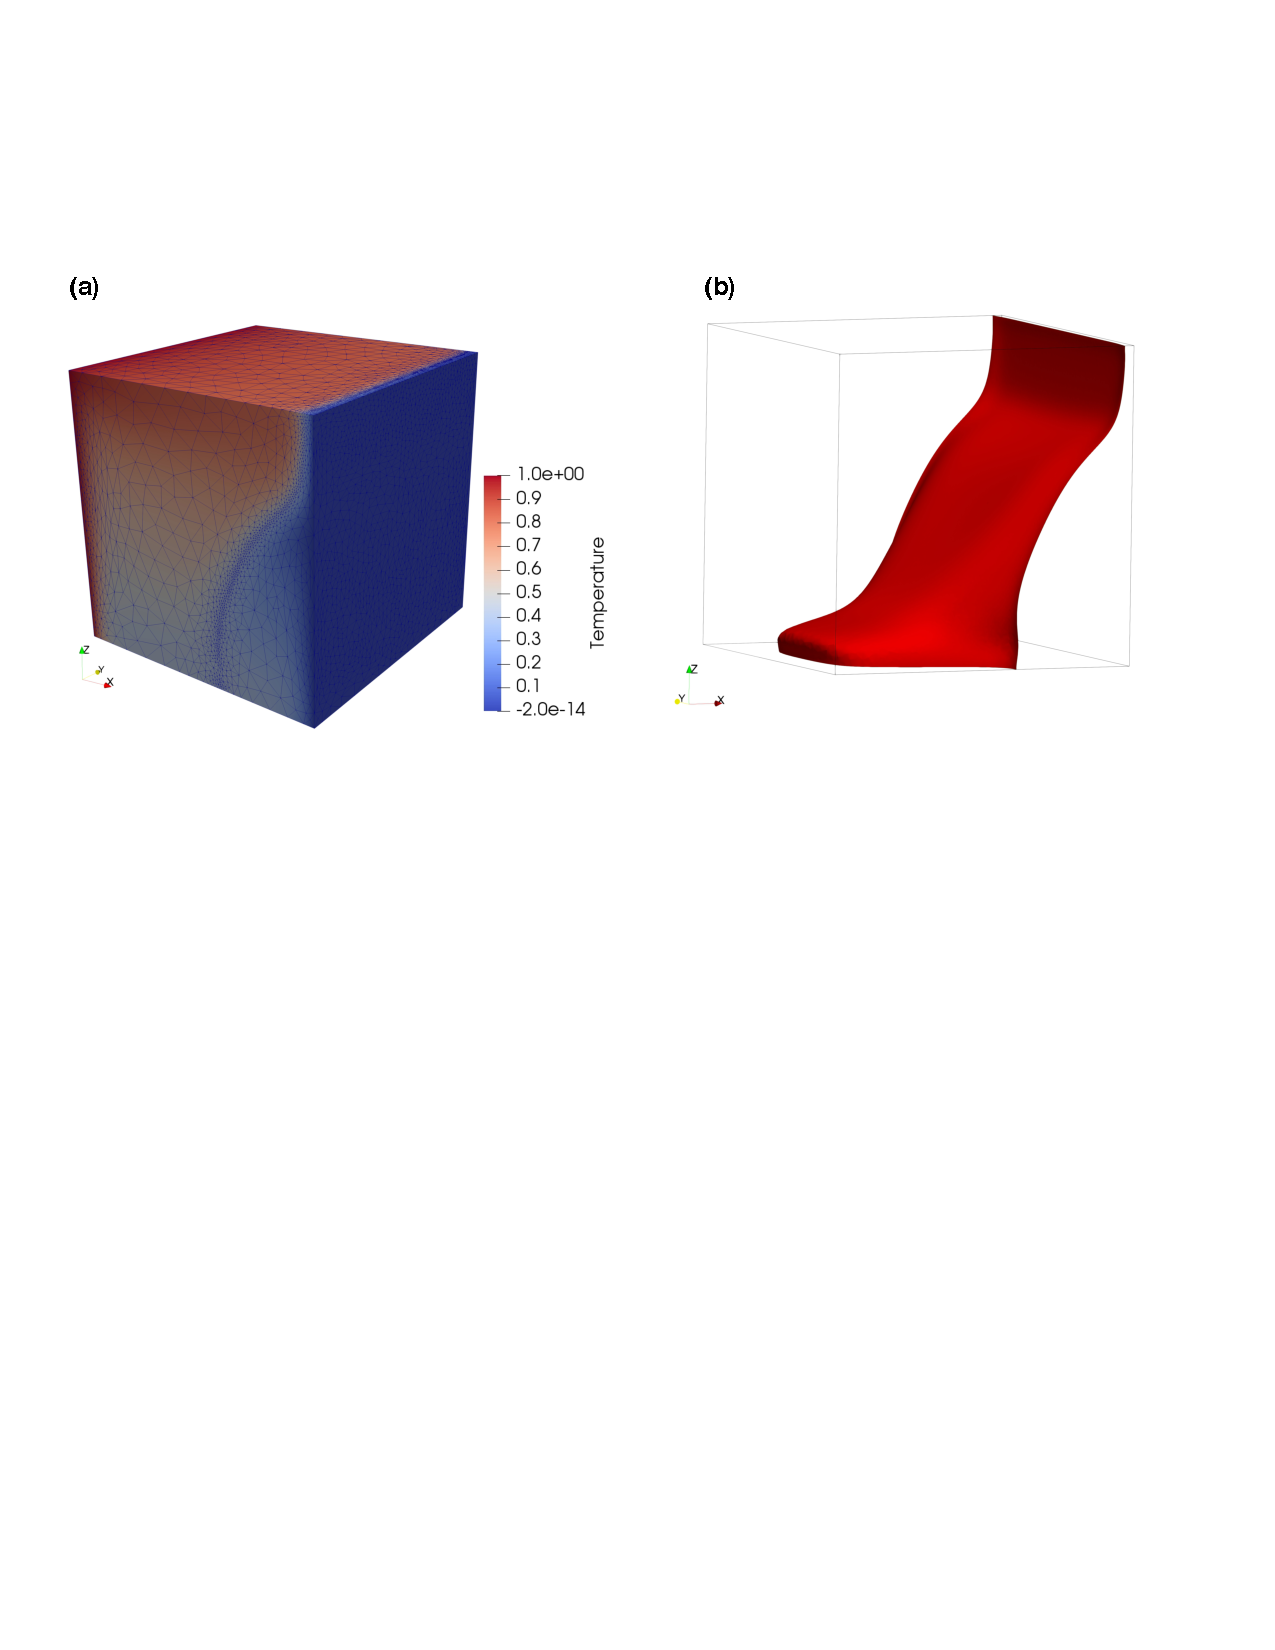
\includegraphics[width=0.9\textwidth]{\figpath/Fig_cap_natconv/3D_WaterConvec}}
 {\includegraphics[width=0.9\textwidth]{\figpath/Fig_cap_natconv/3D_WaterConvec_2}}
\end{minipage}
\end{center}
\caption{3D convection of water in a cube with an inner heated cube. (a) Temperature distribution and adapted mesh. (b) Zoom of the 3D adapted mesh at mid-plane. (c) Iso-surface $\theta = \theta_m$. (d) Comparison of the profile of the vertical velocity along $z-$direction, at the midplane ($y=0.5$) and $x=0.93$ with numerical benchmark by  \cite{Kowalewski-1999}.}
\label{fig-3D_Water_convec} 
\end{figure}

\section{3D numerical simulations of melting with convection}

%%%%%%%%%%%%%%%%%%don't forget if needed %%%%%%%%%%%%%%%%%%%%%
%\section[toc version]{title version%
%              \sectionmark{head version}}
%\sectionmark{head version}
%%%%%%%%%%%%%%%%%%%%%%%%%%%%%%%%%%%%%%%%%%%%%%%%%%%%%%%%%%%%%%
\def\titcourt{Conclusion and perspectives}
\def\titlong{Conclusion and perspectives}
%%%%%%%%%%%%%%%%%%%%%%%%%%%%%%%%%%%%%%%%%%%%%%%%%%%%%%%%%%%%%%%%
\chapter[\titlong]{\titlong%
              \chaptermark{\titcourt}}
\chaptermark{\titcourt}
\label{chap-conclusion}
%%%%%%%%%%%%%%%%%%%%%%%%%%%%%%%%%%%%%%%%%%%%%%%%%%%%%%%%%%%%%%%%
%%%%%%%%%%%%%%%%%%%%%%%%%%%%%%%%%%%%%%%%%%%%%%%%%%%%%%%%%%%%%%%%

In this thesis, we have presented numerical simulations of natural convection with melting boundary.
We have developed numerical tools for simulating $2$ and $3$D configurations of solid-liquid phase-change systems involving natural convection, using adaptive finite elements method.

\noindent The buoyancy-induced fluid motion in the liquid phase was modeled by the incompressible Navier-Stokes equations with Boussinesq approximation. 
The phase-change was modeled by an enthalpy-porosity model using a temperature-based
formulation for the energy conservation equation.
A single-domain method, solving the same system of equations in both phases, including a Carman-Kozeny-type penalty term in the momentum equation, was implemented with the \ff software.

\noindent In the numerical approach, the coupled momentum and energy equations were integrated in time using a fully implicit second-order GEAR scheme. 
The space discretization was based on a Taylor-Hood triangular finite elements, approximating the velocity and the pressure with $\PP_2$ and $\PP_1$ finite elements, respectively.
Since we noticed from the literature review that the published numerical simulations required considerable high computer resources and CPU time, the main feature of our numerical method was the use of mesh adaptivity algorithm using metrics control to adapt the mesh every time step.
We have concentrated the grid refinement effort only in regions displaying high gradients of the computed variables, and prescribed coarser meshes in the solid phase and stagnant regions, thus reducing considerably the degrees of liberty while keeping high accuracy.
The accuracy of the numerical method was tested using manufactured solutions: the expected second-order accuracy in both space and time was obtained.

As a first purpose of the study, we have organized the program as a toolbox for the software \ff.
The toolbox was designed to be an easy-to-use tool to handle phase-change problems.
All technical issues related to the implementation of the finite element method were hidden, allowing to focus on numerical algorithms and their performance.
A sequence of validation tests was performed, and presented by increasing gradually the level of complexity.
Using the provided examples, the user could implement easily similar problems involving phase-change phenomena.

\noindent We first tested the capability of the Navier-Stokes solver to deal with natural convection problems, without enthalpy and porosity terms in the system of equations.
We started by simulating the natural convection of air and water inside differentially heated square enclosures and validated our results against classical benchmarks of classical convection.
Rayleigh numbers up to $10^8$, at the limit of the steadiness for the natural convection of air, were considered.
Additionally, we investigated the thermal driven problem including heated obstacle to assess for the robustness of the code.

\noindent We also computed the natural convection of water, which considers a non-linear variation of the density in the expression of the buoyancy force.
The comparison with existing numerical data in the literature exhibited very good agreement. 
The mesh adaptivity algorithm proved very efficient, allowing to capture accurately the anomalous variation of the density around $T = 4 \, ^oC$.
For all the simulations presented in the frameworks of natural convection problems, the steady state regimes were reached at most after $50$ CPU seconds of computation.

\noindent We then validated extensively the code by simulating the problem of melting and solidification of a PCM.
We first considered the melting of n-octadecane and Gallium inside rectangular enclosures vertically heated to compare our simulation with available experimental and numerical results in the literature.
A mesh convergence test was performed to ensure the grid-convergence of the solution.
The parameters of the adapted mesh, used for all simulations, exhibited a variation lower than $0.042 \%$ for the location of the solid-liquid interface and for the time evolution of the Nusselt number.

\noindent Three Rayleigh numbers ranging from $10^5$ to $10^8$ were considered for the n-octadecane PCM melting, and our simulations were compared with three different benchmarks.
A good agreement was found for the comparison with existing experimental and numerical results.
Concerning the controversial melting of Gallium in $2$D configurations, our simulations exhibited multi-cellular structures of the melted flow and highly oscillating values of the Nusselt number, in agreement with many observations from the literature.

\noindent Moreover, more complex geometries, such as highly distorted domain or cylindrical PCM including inner heated pipes, were also performed.
For all considered cases, a variable mesh in the vicinity of the walls and along the phase-change front, ensured a good capture of the boundary layer region and the location of the interface.
The simulation of the melting of Gallium showed that our simulations run $245$ times faster when compared with the simulations of \cite{hannoun2003resolving}.

\noindent We finally presented the challenging case of water freezing inside a differentially heated cavity.
A qualitative agreement with the experimental image of the solidification front was obtained.
The efficiency of our numerical algorithm allowed to perform simulations for melting problems, from $45$ minutes for the lowest value of $\Ray$ to $5$ hours for $\Ray = 10^8$.
After a thorough investigation, we could conclude that our numerical method was validated by providing a good agreement with the benchmarks presented in the literature, for the natural convection of air and water and for the solid-liquid phase change problems including melting and solidification.

The second purpose of the study was to provide a thorough analysis of the melting and the solidification process and compare with numerical results.

\noindent We first compared the behavior of the melting PCM when the latter is subject to heating from the sides or from below (lateral or basal melting).
For the lateral melting case, we assessed for the influence of the Rayleigh number on the heat transfer,
by computing several configurations using different value of $H$ and $\delta T$.
It was shown that increasing the Rayleigh number by keeping $\delta T$ constant induces a slower melting rate and higher heat transfer.
However, increasing both Rayleigh and Stefan numbers induced an earlier onset of the convection-dominated regime, improving the efficiency of the PCM for a practical application.

\noindent For the basal melting case, we developed a scale analysis during the linear regime and provided a comprehensive description of the heat transfer processes during the melting.
Differences between lateral and basal melting were drawn, mainly for the structure of the flow and the time evolution of the Nusselt number.
A mono-cellular flow was observed for the lateral melting case at any investigated Rayleigh numbers, while natural convection developed in the form of B�nard cells for the basal melting case.
Moreover, the quasi-steady evolution of $\mathcal{N}\!u$ in the frame of a vertical heating is not observed when the PCM is heated from below since high oscillating evolutions were exhibited.

\noindent Further investigation of the solidification process was also addressed by simulating alternate melting and solidification cycles.
Solidification after either complete or partial melting were performed, with an assessment of the melting rate, the heat transfer and the accumulated heat input.
It was observed that convective heat transfer dominated the melting process, enhancing thus the heat transfer, while conduction was the main heat transfer mode during the solidification, resulting to a slower operating process. 
However, when the discharge temperature was decreased by a factor of $5$, the solidification and the melting occur over similar time intervals.
The challenging task for the mesh adaptivity procedure was to track the two moving interfaces during the solidification cycle.

The third purpose of the thesis was to expand the numerical simulation to $3$D configurations.
Parallel $3$D tools for melting or solidification purpose involving natural convection flow, using domain decomposition method were presented.
The numerical simulations were carried out using the recent library \texttt{ffddm} in \ff.
The originality of our numerical approach was the use of 3D adaptive mesh, performed every time steps, using \textit{mmg3d} library.
We used \textit{Metis} library to split the domain into subdomains.
The linear system of equations resulting from the Newton linearization was solved using parallel \textit{GMRES} Krylov methods.

\noindent We first validated the natural convection of air and water inside cubic enclosures and found good agreement with classical benchmarks.
We also simulated the melting of n-octadecane PCM and the difficult case of water freezing inside differentially heated cubic cavity.
The influence of the three-dimensional effects on the flow, that was neglected in $2$D simulations, was highlighted by the $3$D shape of the solid-liquid interface. 
Iso-surfaces of the temperature were also impacted by the secondary flow in the vicinity of the side walls.
The adaptive $3$D mesh procedure proved very efficient to capture several interfaces, as in the case of the water freezing. \\

\textbf {Perspectives}\\

One of the major limitation of the present physical model is that we neglected the undercooling phenomenon, since we assumed the temperature of fusion and the temperature of solidification equal for all simulations.
Though, the liquid could solidify at a temperature significantly lower than the melting temperature, because of a  problem of nucleation at the microscopic scale.
An enthalpy-based formulation of the enthalpy-porosity model should be implemented to this end, since the undercooling problem can not be implemented in the current temperature-based approach.
Additionally, a microsegregation model and a coupling relationship between thermal and solute equations could be implemented in the code, in order to be able to simulate solidification or melting of binary mixtures.
Such models would allow to simulate more complex configurations such as dendritic formations during the solidification process.

While the Boussinesq approximation proved to be robust for the considered configuration in this study, the assumption of constant thermo-physical properties limits the range of material that could be simulated by our code.
A variable density code could be a valuable tool to investigate a larger type of PCM and more industrial configurations.

Concerning the numerical model, the second order GEAR scheme provided accurate solutions for all the considered simulations.
Furthermore, a variable time step scheme would increase the robustness of the numerical method.
The simulation of the melting PCM require for example a small time steps during the initialization stage, while larger time steps could be prescribed later in the simulation.
Adapting automatically this procedure will increase considerably the efficiency of the code.
For the solidification problem, new boundary conditions could be further developed by using some models that take into account realistic boundary conditions.

For the parallel algorithm, other preconditionners and solvers should be investigated.
This is not a difficult task with \ff since the software is interfaced with popular MUMPS, PETSc, or HPDDM solvers.







%%%%%%%%%%%%%%%%%%%don't forget if needed %%%%%%%%%%%%%%%%%%%%%
%\section[toc version]{title version%
%              \sectionmark{head version}}
%\sectionmark{head version}
%%%%%%%%%%%%%%%%%%%%%%%%%%%%%%%%%%%%%%%%%%%%%%%%%%%%%%%%%%%%%%
\def\titcourt{ }
\def\titlong{ }
%%%%%%%%%%%%%%%%%%%%%%%%%%%%%%%%%%%%%%%%%%%%%%%%%%%%%%%%%%%%%%%%
%\chapter[\titlong]{\titlong%
%              \chaptermark{\titcourt}}
%\chaptermark{\titcourt}
%\label{chap-MELTING-CAVITY}


\chapter{Appendix} \label{chap-Appendix}
%%%%%%%%%%%%%%%%%%%%%%%%%%%%%%%%%%%%%%%%%%%%%%%%%%%%%%%%%%%%%%%%
%%%%%%%%%%%%%%%%%%%%%%%%%%%%%%%%%%%%%%%%%%%%%%%%%%%%%%%%%%%%%%%%

\section{Boundary layer approximation and scale analysis} \label{sec-bound-scal-anal}
Either PCM is used for energy storage or for building insulation or for other purposes, one would necessarily assess the heat transfer during the phase-change process.
Mainly, it was extensively proven that the convective heat transfer plays significant role during the melting stage.
Therefore, before solving numerically eqs. (\ref{eq-qmvt}) - (\ref{eq-energ}), we first rely on scale analysis to predict theoretically the fluid flow and heat transfer patterns that can develop in the fluid part.
The idea behind the scaling analysis is about identifying the proper scales of the phenomenon, in order to understand the evolution of the heat transfer and the melting rates.

In the present analysis, we will consider first only the liquid phase without phase-change.
A further analysis of the scale during the melting will be developed in sec. (\ref{chap-MELTING-CAVITY}).
We consider a two-dimensional enclosure of height H filled with Newtonian fluid, differentially heated from the vertical walls and insulated from the horizontal walls.
A No-slip boundary condition is considered for the velocity. 
Since no external force is applied to our system, the fluid flow is merely driven by natural convection flow, induced by temperature differences from the vertical walls.
It is well-known from the foregoing boundary conditions that the fluid layer situated close to the vertical walls stuck to the wall and are motionless.
The heat transfer through the fluid layer immediately adjacent to the wall is accordingly by pure conduction, i.e, $ q = - \left. (\partial \theta/ \partial x) \right |_{x=0} $.
We therefore define the average Nusselt number to quantify the heat transfer rate at the heated wall:
\begin{equation}\label{eq-def-Nu}
   N\!u = - \int_0^1 \left. \frac{\partial \theta}{\partial x} \right |_{x=0} dy.
\end{equation}

When a steady state could be reached, the fluid near each sidewall is characterized by two boundary layers: a thermal boundary layer of thickness $\delta_{\theta}$ and a viscous boundary layer of thickness $\delta_\nu$.
The boundary layer approximation assumes that the flow and the energy transfer are restricted predominantly to the boundary layer region.
This theory was proposed first by Prandtl in 1904 and validated later by many experimental and numerical studies.
The main consequences of the boundary layer approximations are that: \\
{\it (i)} the normal part of the momentum equation has a negligible importance, \\
{\it (ii)} the downstream diffusion term in the momentum and energy equations are neglected in comparison with the normal diffusion terms ($\partial^2 \vec{u}/\partial y^2 \ll \partial^2 \vec{u}/\partial x^2$ and $\partial^2 T/\partial y^2 \ll \partial^2 T/\partial x^2$) since the boundary layer thickness is much smaller than the enclosure height ($ \delta \ll H$), \\
{\it (iii)} the pressure distribution is purely hydrostatic, i.e, $P = - \rho g y$, \\
{\it (iv)} the thermal and the viscous boundary layer thickness are given by the order of magnitude expressions: $\delta_\nu/\delta_\theta = o \left(\Pr^{1/2} \right)$.\\
These assumptions lead to the following boundary layer equations for the conservation of mass, momentum and energy:
\begin{eqnarray} \label{eq-bound-mass}
	\frac{\partial u}{\partial x} + \frac{\partial v}{\partial y} &=& 0, \\  \label{eq-bound-mom}
	u \frac{\partial v}{\partial x} + v \frac{\partial v}{\partial y} &=& \nu \frac{\partial^2 v}{\partial x^2} + g \beta (T - T_{ref}), \\ \label{eq-bound-energy}
	u \frac{\partial T}{\partial x} + v \frac{\partial T}{\partial y} &=& \alpha \frac{\partial^2 T}{\partial x^2}. 
\end{eqnarray}
The mass conservation in eq. (\ref{eq-bound-mass}) in the boundary layer region leads to:
\begin{equation}
	\frac{u}{\delta_\theta} \sim \frac{v}{H}.
\end{equation}
The energy eq. (\ref{eq-bound-energy}) expresses a balance between longitudinal convection and transverse conduction:
\begin{equation}
	\frac{v}{H} \sim \frac{\alpha}{\delta_\theta^2},
\end{equation}
which yields:
\begin{equation} \label{eq-scale-v}
	v \sim \frac{\alpha H}{\delta_\theta^2}.
\end{equation}
As far as momentum eq. (\ref{eq-bound-mom}) is concerned, we could identify the interplay among three forces:
\begin{equation} \label{eq-scale-momentum}
	\underbrace{\frac{v^2}{H}}_{inertia} \quad \underbrace{\nu \frac{v}{\delta_\theta^2}}_{friction} \quad \underbrace{g \beta \delta T}_{buoyancy}.
\end{equation}
Using the expression of $v$ in eq. (\ref{eq-scale-v}) and by dividing eq. (\ref{eq-scale-momentum}) by $g \beta \delta T$, we obtain:
\begin{equation} \label{eq-final-scale}
	\underbrace{\left( \frac{H}{\delta_\theta} \right)^4 Pr ^{-1} \Ray^{-1}}_{inertia} \quad  \underbrace{\left( \frac{H}{\delta_\theta} \right)^4 \Ray^{-1}}_{friction} \quad \underbrace{1}_{buoyancy}.
\end{equation}
Eq. (\ref{eq-final-scale}) indicates that the behaviour of the fluid in the boundary layer depends on the $\Pr$ number. \\
First, for a high-Prandtl fluid ($\Pr \geq 1$), the friction-buoyancy balance yields: 
\begin{equation} \label{eq-scale-nbd-high-Pr}
	\delta_\theta \sim H \Ray^{-1/4}.
\end{equation}
The Nusselt number from eq. (\ref{eq-def-Nu}) scales as $H/\delta_\theta$, resulting: 
\begin{equation}
	N\!u \sim Ra^{1/4}
\end{equation}
and $v \sim \alpha/H \Ray^{1/2}$. \\
Second, for a low-Prandtl fluid ($\Pr \ll 1$), we observe a balance between inertia and buoyancy, leading to:
\begin{equation} \label{eq-corr-Low-Pr}
	\delta_\theta \sim H Pr^{-1/4} \Ray^{-1/4}.
\end{equation}
Accordingly we obtain a Nu-Ra correlation:
\begin{equation}
	Nu \sim Pr^{1/4} \Ray^{1/4}.
\end{equation}


%%%%%%%%%%%%%%%%%%%%%%%%%%%%%%%%%%%%%%%%%%%%%%%

%%%%%%%%=====================================================
%\part{Bibliography}
%\parttoc
%%%%%%%=====================================================
\addcontentsline{toc}{chapter}{Bibliography}

\bibliographystyle{\stypath/plainnat-io}
%\bibliographystyle{plain}
%\renewcommand{\bibname}{\em }
\bibliography{\bibpath/bib_thesis_2}
\end{document}
